% !TEX root = ../Main.tex

\chapter[Methods for Simulating Stabilizer Circuits]{Methods for Simulating Stabilizer\\ Circuits}
\label{chap:stabilizers}

\section{Introduction}\label{sec:stabilizer-intro}
% Stabilizer circuits are an intersting class of circuits
% Capture many seemingly quantum features
% Recap definition
% Some of this is probably meant for intro instead
In Section~\ref{sec:intro_efficient_simulations}, we briefly introduced the notion of stabilizer circuits as a class of efficiently simulable quantum computations. In this chapter, we revisit stabilizer circuits in detail, with a focus on different classical data structures for encoding stabilizer states and the corresponding algorithms for simulations.\par
Several informal definitions of stabilizer circuits have been used in the quantum computing literature~\cite{VandenNest2008,Gottesman1998b,Aaronson2004,Seddon2019}. However, what each definition has in common is that they consider Abelian subgroups $\mathcal{S} \subseteq \mathcal{P}_{n}$. These groups $\mathcal{S}$ are also called stabilizer groups. Operations in the circuits have the property that they either leave these groups unchanged, or map them to new groups $\mathcal{S'}\subseteq \mathcal{P}_{n}$.\par
We focus exclusively on stabilizer circuits acting on pure states $\ket{\phi}$ called stabilizer states, which are entirely characterized by their associated stabilizer group
\begin{equation}
    s\ket{\phi}=\ket{\phi}\;\forall s\in\mathcal{S}
\end{equation}
For an $n$-qubit state, the group $\mathcal{S}$ has $2^{n}$ elements~\cite{Gottesman1998b}. As $\mathcal{S}$ is also Abelian, this means it can itself be efficiently described by a set of $n$ independent generators  
\begin{equation}
    \mathcal{S} = \langle g_{1}, g_{2},\dots,g_{n}\rangle \; : g_{i}\in\mathcal{S},
\end{equation}
which are commonly referred to as the `stabilizers' of the state $\ket{\phi}$. We also note that this definition allows us to write
\begin{equation}
    \ketbra{\phi} = \frac{1}{2^{n}}\sum_{s\in\mathcal{S}} s = \frac{1}{2^{n}}\prod_{i=1}^{n}\left(\mathbb{I}+g_{i}\right)
\end{equation}
As stabilizer circuits map stabilizer states to other stabilizer states, this means they must be built up of unitary operations which map Pauli operators to other Pauli operators under conjugation. This set is commonly denoted as $\mathcal{C}$, and alternatively referred to as $\mathcal{C}_{2}$, the `second level of the Clifford hierarchy':
\begin{align}
    \mathcal{C}_{2} &\equiv \{V\,:\,VPV^{\dagger}\in\mathcal{P}_{n}\;\forall P\in\mathcal{P}_{n}\} \label{eq:c2}\\
    \mathcal{C}_{j} &\equiv \{U\,:\,UPU^{\dagger}\in\mathcal{C}_{j-1}\;\forall P\in\mathcal{P}_{n}\} \label{eq:cj}
\end{align}
where in Eq.~\ref{eq:cj} we have also introduced the (recursive) definition for level $j$ of the Clifford hierarchy. For concreteness, we define level $1$ of the hierarchy as $\mathcal{C}_{1}=\mathcal{P}_{n}$.\par
From this definition, applying a Clifford unitary $V$ updates the stabilizer group as
\begin{equation}
    V\mathcal{S}V^{\dagger}=\langle Vg_{i}V^{\dagger}\rangle = \langle g_{i}' \rangle = \mathcal{S}'
\end{equation}
%TODO: Do we need to explain measurement or just cite it? Maybe this comes up later in the implementation...
We also allow stabilizer circuits to contain non-unitary operations, in the form of measurements in the Pauli basis~\cite{Gottesman1998b}.
\subsubsection{Simulating stabilizer circuits}
% Classical simulabiltiy follows from gate updates and encoding
% Introduce tableaux, and classical encoding
From the above definitions, we can see that simulating a stabilizer circuit on $n$ qubits corresponds to updating the $n$ stabilizer generators for each unitary and measurement we apply. As the number of generators grows linearly in the number of qubits, if these updates can be computed in time $O\left(\poly (n)\right)$ it follows the circuits can be efficiently simulated clasically.\par
The first proof of this was given by Gottesman in~\cite{Gottesman1998b}, by showing through examples that stabilizer updates can be quickly computed for the CNOT, H and S gates, and for single qubit Pauli measurements. The $n$ qubit Clifford group, $\mathcal{C}_{2}$, is entirely generated from these gates, and thus any Clifford operation can also be efficiently simulated. This result is typically referred to as the `Gottesman-Knill' theorem.\par
A more formal proof follows from the work of Dehaene \& de-Moore, who showed that the action of Clifford unitaries on Pauli operators corresponds to multiplication of $(2n+1)\times (2n+1)$ symplectic binary matrices with $(2n+1)$-bit binary vectors~\cite{Dehaene2003}. The dimension of these elements also grows just linearly in the number of qubits, and as matrix multiplication requires time $O(n^{2.37})$ it follows that we can update the stabilizers in $O(mn^{2.73})$ for $m$ Clifford gates.\par
This work was extended by Aaronson \& Gottesman, who introduced an efficient data structure for stabilizer groups, and algorithms for their updates under Clifford gates and Pauli measurement~\cite{Aaronson2004}. This method avoids the need for matrix multiplications, instead providing direct update rules allowing stabilizer circuits to be simulated in $O(n^{2})$.\par
Since 2004, there have been several papers looking at different data structures and algorithms for simulating stabilizer circuits of the type we consider here. For example, a method based on encoding stabilizer states as graphs~\cite{Anders2006}, refinements of the Aaronson \& Gottesman encoding~\cite{Garcia2012}, and an encoding using affine spaces and phase polynomials~\cite{VandenNest2008,Bravyi2016}.\par
In the rest of this section, we will discuss different aspects of simulating stabilizer circuits, focusing on updating stabilizer states under gates and measurements, computing stabilizer inner products, and the connections between stabilizer circuits and states.
% \clearpage
\subsection{Tableau Encodings of Stabilizer States}\label{sec:sympencoding}
The method in \cite{Aaronson2004} is based on a classical data structure the authors call the `stabilizer tableau', a collection of Pauli matrices that define the stabilizer group, encoded using the binary symplectic representation of \cite{Dehaene2003}
\begin{equation} P = \left(-1\right)^{\epsilon} \mathi^{\delta}\bigotimes_{i=1}^{n} x_{i}z_{i}\end{equation}
where the Pauli matrix at qubit $i$ is defined by two binary bits such that
\begin{equation}
    x_{i}z_{i} = \begin{cases}
    I & x_{i}=z_{i}=0\\
    X & x_{i}=1, z_{i}=0 \\ 
    Z  &x_{i}=0, z_{i}=1 \\
    Y  &x_{i}=z_{i}=1
    \end{cases}
\end{equation}
Together with the $\delta$ and $\epsilon$ phases, a generic Pauli operator can be encoded in $2n+2$ bits; two bits to encode the phase, and two $n$-bit binary strings $\va{x},\va{z}\in\mathbb{Z}_{2}^{n}$ to encode the Pauli acting on each qubit, commonly referred to as `x-bits' and `z-bits' respectively. In this picture, multiplication of Pauli operators corresponds to addition of $\va{x}$ and $\va{z}$ bits modulo 2, with some additional, efficiently computable function for correcting the phase~\cite{Dehaene2003}.
\begin{align}
    P Q &= i^{\delta_{pq}}-1^{\epsilon_{pq}}\bigotimes_{i=1}^{n}x_{i}' z_{i}' \\
    x'_{i} &= x_{pi}\oplus x_{qi} \\
    z'_{i} &= z_{pi} \oplus z_{qi}
\end{align}
where $\delta_{pq} = \delta_{p}\oplus \delta_{q}$, $\epsilon_{qr} = f(\va{x}_{p}, \va{z}_{p}, \va{x}_{q}, \va{z}_{q})$.\par
%%Tableau definition, drops an extra factor of n bits
%% Gate updates
In stabilizer groups, we can restrict ourselves to considering Pauli operators with only a real phase. This is because if $iP\in\mathcal{S}$, then $(iP)^{2}=-I\in\mathcal{S}$. But, this implies that $-I\ket{\phi}=\ket{\phi}$, which can only be satisfied by the null vector.\par
While only $n$ generators $S_{i}$ are needed to characterize the stabilizer group $\mathcal{S}$, the tableau also includes an additional $2n$ operators called `destabilizers' $D_{i}\in\mathcal{P}_{n}$. Together, these $2n$ operators generate all $4^{n}$ elements of $\mathcal{P}_{n}$. Including this additional information speeds up the task of simulating stabilizer circuits with this representation, at the expense of a doubling of the memory requirements.\par
There are many possible choices of destabilizer, but the tableau chooses operators such that~\cite{Aaronson2004}
\begin{align*}
    \comm{D_{i}}{D_{j}} &= 0\;\forall\, i, j \,\in \{1,\dots,n\} \\
    \comm{D_{i}}{S_{j}} &= 0 \iff i\neq j \\
    \acomm{D_{i}}{S_{i}} &= 0 
\end{align*}
Altogether, the full tableau has spatial complexity $4n^{2}+2n$. These are sometimes referred to as `Aaronson-Gottesman' tableaux or `CHP' tableaux, after the software implementation by Aaronson~\cite{Aaronson2004b}.
\begin{figure}[H]
\begin{equation}
\kbordermatrix{~ & ~ & ~ & ~ & ~ & ~ & ~ & ~ & ~ & ~\\
    \mathcal{D}_{1} & x_{1,1} & \cdots & x_{1,n} & \omit\vrule & z_{1,n} & \cdots & z_{1,n} & \omit\vrule & r_{1} \\
    \vdots & \vdots & \ddots & \vdots &\omit\vrule & \vdots & \ddots & \vdots & \omit\vrule  &\vdots \\
    \mathcal{D}_{n} & x_{n,1} & \cdots & x_{n,n} & \omit\vrule & z_{n,1} & \cdots & z_{n,n} & \omit\vrule & r_{n}\\ \hline
    \mathcal{S}_{1} & x_{n+1,n} & \cdots & x_{n+1,n} & \omit\vrule & z_{n+1,1} & \cdots & z_{n+1,n} & \omit\vrule & r_{n+1}\\
    \vdots & \vdots & \ddots & \vdots & \omit\vrule & \vdots & \ddots & \vdots & \omit\vrule & \vdots \\
    \mathcal{S}_{n} & x_{2n, 1} & \cdots & x_{2n, n} & \omit\vrule & z_{2n,1} & \cdots & z_{2n,n}&\omit\vrule&r_{2n}
    }
\end{equation}
\caption{Example of a `CHP' tableau, where the first $n$ rows are the Destabilizers and the next $n$ rows are the stabilizers. The $2n+1$th column gives the phase $-1^{r_{i}}$ for each operator.}
\label{fig:ExampleCHP}
\end{figure}
\subsubsection{Simulating Gates}
Gate updates for each individual operator in the tableau can be computed constant time. For example, the Hadamard transforms single qubit Pauli matrices under conjugation as
\begin{equation}
    HPH^{\dagger} = \begin{cases}
        I & P=I\\
        Z & P=X\\
        X & P=Z\\
        -Y & P=Y
        \end{cases}
\end{equation}
In the symplectic form, we then have to update the $i$th Pauli operator as
\begin{equation}
    p = x_{i} \oplus z_{i} \Rightarrow \begin{array}{lcr}
    x_{i}' & = & \left(x_{i}\oplus p\right)\\
    z_{i}' & = & \left(z_{i}\oplus p\right) 
    \end{array}
\end{equation}
and the phase as
\begin{equation}
\delta' = \delta \oplus \left(x_{i}\wedge z_{i}\right)
\end{equation}
Similar update rules exist for the CNOT and S gates, which together generate the $n$ qubit Clifford group. As there are $O(n)$ operators in the tableau, and each update is constant time, gate updates overall take $O\left(2n\right)$~\cite{Aaronson2004}. This is in contrast to the $O(n^{2.37})$ complexity of~\cite{Dehaene2003}.
\subsubsection{Simulating Measurements}
The addition of the destabilizer information is  used to speed up the simulation of Pauli measurements on Stabilizer states. Measuring some operator $P$ on a stabilizer state will always produce either a deterministic outcome, or an equiprobable random outcome~\cite{Gottesman1998b}.\par
If the outcome is deterministic, then $\pm P$ is in the stabilizer group, and the outcome is $+1$ or $-1$ respectively. Using the stabilizer generators, this allows us to write 
\begin{equation}
    \comm{P}{S_{i}}=0\;\forall S_{i}\in\mathcal{S} \implies \prod_{i}c_{i}S_{i} = \pm P. \label{eq:det_requirement}
\end{equation}
for binary coefficients $c_{i}$.\par
Checking if the outcome is deterministic takes $O(n^{2})$ time in general, using the symplectic inner product to check the commutation relations~\cite{Dehaene2003}. However, checking which measurement outcome occurs involves computing the coefficients $c_{i}$. In the symplectic form, this can be rewritten as
\[
    A\va{c}=P
\]
where $\va{c}$ is a binary vector, $A$ is a matrix with each stabilizer as a column vector, $P$ is the operator to measure, and we have dropped the phase~\cite{Aaronson2004}. Solving this would require inverting the matrix $A$, and take time $O(n^{3})$.\par
Aaronson \& Gottesman show that for single qubit measurements, including destabilizer information instead allows us to compute the $c_{i}$ and the resulting measurement outcome in $O(n^{2})$. As this is a single qubit measurement, they also show that the commutativity relation requires checking only individual bits of the stabilizer vectors, also reducing that step to $O(n)$ time.\par
For random measurements, from Eq.~\ref{eq:det_requirement}, $\exists S_{i}:\acomm{S_{i}}{P}=0$, and it suffices to replace this stabilizer with $P$, and update the other elements of the group as $S_{j}'=PS_{j}$ iff $\acomm{S_{j}}{P}=0$~\cite{Gottesman1998b,Aaronson2004}.
\subsubsection{`Canonical' Tableaux}
% A&G fix tableaux through initial state
There are multiple possible choices of generators for each stabilizer group/state. For example, the stabilizer group for the Bell state $\ket{\phi^{+}}=\frac{1}{2}\left(\ket{00}+\ket{11}\right)$ can be written as
\begin{align}
    \mathcal{S} = \{II, XX, -YY, ZZ\} = \langle XX,-YY\rangle = \langle XX, ZZ\rangle = \langle -YY,ZZ\rangle.
\end{align}
In simulation, tableau are fixed by choice of a convention. For example, it is possible to arrive at a `canonical' set of stabilizer generators using an algorithm which strongly resembles Gaussian elimination~\cite{Garcia2012}. This method rearranges the stabilizer rows of the tableau by multiplying and swapping generators, such that the overall stabilizer group is left unchanged. Computing this canonical form requires  time $O(n^{3})$~\cite{Garcia2012}.
\begin{figure}[H]
    \centering
    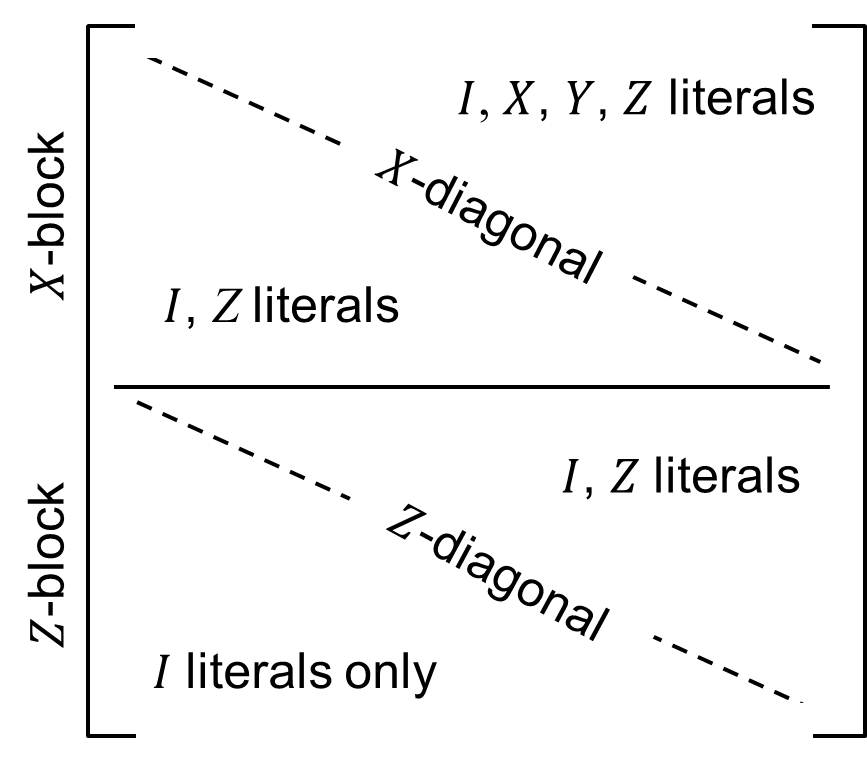
\includegraphics[width=0.45\linewidth]{stbmtx_inv.jpg}
    \caption{Representation of the canonical or `row-reduced' set of stabilizer generators. Figure taken from~\cite{Garcia2012}.}
\label{fig:canoncialtableau}
\end{figure}
These tableau can then be updated using the same methods as in~\cite{Aaronson2004}, though this will in general not preserve the canonical form. Each Clifford gate will change one or two columns of the tableau, and thus an additional $O(n)$ row multiplications are required to restore it to canonical form, taking total time $O(n^{2})$ per gate~\cite{Garcia2015}.
Importantly, this canonical tableau can also be used to compute deterministic measurement outcomes in time $O(n)$, and so this method can simulate measurement outcomes more efficiently at the cost of more expensive gate updates~\cite{Garcia2015}.\par
In contrast, Aaronson \& Gottesman fix the stabilizer tableau through an initial state, $\ket{\va{0}}$. The full tableau for this state looks like the identity matrix, with an additional zero-column for the phases. The tableau of a given state $\ket{\phi}$ is then built up gate by gate using a stabilizer circuit $V:\ket{\phi}=V\ket{\va{0}}.$
\subsection{Connecting Stabilizer States and Circuits}
% Connection between clifford circuits and states
The convention for the `CHP' stabilizer tableaux mentioned above, and the definition of stabilizer circuits given in Section~\ref{sec:stabilizer-intro}, show that stabilizer states can also be defined by a stabilizer circuit and an initial state.\par
In~\cite{Aaronson2004}, the authors derive examples of these `canonical circuits', and show that its possible for any stabilizer state to be synthesised by a unique circuit acting on the $\ket{\va{0}}$ state
\begin{equation}
    \ket{\phi} = V\ket{\va{0}} = H\;C\;S\;C\;S\;C \;H \; S \;C \;S \ket{\va{0}}\label{eq:chpcirc}
\end{equation}
where each letter denotes a layer made up of only Hadamard (H), CNOT (C) or S gates. The proof is based on  a sequence of operations reducing an arbitrary tableau to the identity matrix, each step of which corresponds to applying layers of a given Clifford gate~\cite{Aaronson2004}. As a corollary, the total number of gates in the canonical circuit for an $n$-qubit stabilizer state scales as $O(n\log (n))$~\cite{Aaronson2004}, based on previous work on synthesising CNOT circuits with the $O(n\log (n))$ gates~\cite{Patel2003}, and that each H and P layer can act on at most $n$-qubits.\par
A simpler canonical form was derived in 2008, which allows a stabilizer circuit to be written as
\begin{equation}
    \ket{\phi} = S\;CZ\;X\;C\;H \ket{\va{0}} \label{eq:affinecirc}
\end{equation}
where the CZ and X layers are made up of Controlled-Z gates and Pauli X gates, respectively~\cite{VandenNest2008}. This circuit follows from the work of~\cite{Dehaene2003}, who showed that any stabilizer state can be written as
\begin{equation}
    \ket{\phi} = \frac{1}{\sqrt{2^{k}}}\sum_{x\in\mathcal{K}} i^{f(\va{x})}\ket{\va{x}}.\label{eq:affineform}
\end{equation}
In this equation, $\mathcal{K}\subseteq\mathbb{Z}_{2}^{n}$ is an affine subspace of dimension $k$, and $f(\va{x})$ is a binary  function evaluated $\bmod \,4$. Thus, a stabilizer state is always a uniform superposition of computational basis strings, with individual phases $\pm \mathi,\,\pm 1$. The affine space $\mathcal{K}$ has the form
\[
    \mathcal{K}=\{G\va{u} + \va{h}\}
\]
for $k$-bit binary vectors $\va{u}$, an $n\times k$ binary matrix G, and an $n$-bit binary `shift-vector' $\va{h}$.\par
Van den Nest~\cite{VandenNest2008} notes that this representation can be directly translated into a stabilizer circuit; we begin by applying $H$ to the first $k$ qubits to initialize the state $\sum_{\va{u}}\ket{\va{u}}\otimes\ket{0^{\otimes n-k}}$. We then apply CNOTs to prepare $\sum_{\va{u}}\ket{G\va{u}}$, and finally Pauli Xs to prepare $\sum_{\va{u}}\ket{G\va{u}\oplus \va{h}}$.\par
The phases can be further decomposed into two linear and quadratic binary functions $l,q\,:\mathbb{Z}_{2}^{n}\rightarrow\mathbb{Z}_{2}$, such that $i^{q(\va{x})}=i^{l(\va{x})}(-1)^{q(\va{x})}$. The linear terms correspond to single qubit phase gates, which can be generated by the S gate, and the quadratic terms to two-qubit phase gates, generated by the CZ~\cite{VandenNest2008}. Thus,
\begin{equation}
\ket{\phi}=\sum_{\va{x}\in\mathcal{K}}i^{l(\va{x})}(-1)^{q(\va{x})}\ket{\va{x}} = S\;CZ\;X\;C\;H\;\ket{\va{0}}
\label{eq:expandedaffinecirc}
\end{equation}
While~\cite{VandenNest2008} showed that these simpler canonical circuits exist, an algorithm to compute them first introduced in 2012~\cite{Garcia2012}. This method allowed such a circuit to be read off from the `canonical' set of stabilizer generators introduced in Section~\ref{sec:sympencoding}. 
\subsection{Computing Inner Products}\label{sec:innerproduct}
%% Outline inner product complexity as it comes up a lot later, cite BG for affine space, mention CHP/Canonical
The final task we might consider in simulating stabilizer circuits is the problem of computing probability amplitudes $P(\va{x})=\left\vert \braket{\va{x}}{\phi}\right\vert^{2}$. As computational states are also stabilizer states, this corresponds more broadly to computing inner products between stabilizer states.\par
From the affine space form in Eq.~\ref{eq:affineform}, we can see that
\begin{equation}
\braket{\varphi}{\phi} = \frac{1}{\sqrt{2^{k+k'}}}\sum_{\va{x}\in\mathcal{K}\cap\mathcal{K'}} i^{f(\va{x})-f'(\va{x})}\label{eq:affine_ip}
\end{equation}
and the problem of computing the inner product corresponds to computing the magnitude of an `exponential sum' of phase differences $(\pm\mathi,\;\pm 1)$ for each string $\va{x}$ in the intersection of the two affine spaces~\cite{Bravyi2016}. As each term in the sum has amplitude $\frac{1}{\sqrt{2}}$ and as terms $\pm \mathi, \pm 1$ can cancel, we can see that
\[
\left\vert \sum_{\va{x}} i^{f(\va{x})-f'(\va{x})}\right\vert = \begin{cases}
0 \\
2^{s/2} : s\in \{0,1,\dots,n\}
\end{cases}
\]
This sum can be solved in $O(n^{3})$ time, using an algorithm developed by Sergey Bravyi~\cite{Bravyi2016,Bravyi2018,Bravyi2017}. An algorithm for computing this intersection was also described in~\cite{Bravyi2016}, which we discuss further in Section~\ref{sec:stabilizer_simulators}.\par
Alternatively, the inner product can also be computed using the stabilizer generators directly. Consider two states $\ket{\phi},\ket{\varphi}$ with respective generators $G_{i},H_{i}$. If $\exists i,j\,:G_{i}=-H_{j}$, the states are orthogonal and the inner product is $0$. Otherwise, the inner product is given by $2^{-s}$, where $\va{s}$ the number of generators $G_{i}\notin \{H_{i}\}$.\par
While there are multiple choices of stabilizer generators, we note that inner products are invariant under unitary operations $U$ as
\[
\braket{\varphi}{\phi} = \matrixel{\varphi}{U^{\dagger}U}{\phi}.
\]
Thus, given the canonical circuit $V\; : \ket{\varphi}=V\ket{\va{0}}$
\[
\braket{\varphi}{\phi} = \matrixel{\varphi}{V^{\dagger}V}{\phi} = \matrixel{\va{0}}{V}{\phi}.
\]
%Gaussian elimination
Each stabilizer $G_{i}'$ of $\ket{\va{0}}$ has a single Pauli $Z$ operator acting on qubit $i$. By simplifying the stabilizer $H_{i}'$ of $V\ket{\phi}$ using Gaussian elimination, then we have
\begin{equation}
\left\vert \matrixel{\va{0}}{V}{\phi}\right\vert = \begin{cases}
 0 & \exists H_{i}' = \bigotimes_{i}Z_{i}\\
 2^{-s} & \exists H_{i}' : \acomm{H_{i}'}{G_{i}'} = 0
\end{cases}
\end{equation}
where $s$ is the number of stabilizers that anticommute with the corresponding stabilizer $G_{i}'$~\cite{Aaronson2004}. The second case arises as if $\acomm{H_{i}'}{G_{i}'} = 0$, then $H_{i}'$ acts as either Pauli $X$ or $Y$ on qubit $i$. Thus, the qubit is in state $\ket{\pm 1}$ or $\ket{\pm\mathi}$, and $\braket{0}{\pm i,1}=\frac{1}{\sqrt{2}}$. Because this method involves computing the canonical circuit and then applying Gaussian elimination, it runs in time $O(n^{3})$.\par
The first implementation of this algorithm was given in~\cite{Garcia2012}, where the authors first use their canonical form to construct a `basis circuit' $B : \ket{\varphi}=B\ket{\va{b}}$ for some computational state $\ket{\va{b}}$, and then compute $\matrixel{\va{b}}{B}{\phi}$ using the same method outlined above~\cite{Garcia2012}.
\section{Results}
The main result of this chapter is to introduce two new classical representations of stabilizer states developed in collaboration with Sergey Bravyi~\cite{Bravyi2018}. We will discuss their algorithmic complexity, and implementation in software. We will also briefly discuss the implementation of a classical data-structure based on affine spaces, introduced in~\cite{Bravyi2016}.\par
Finally, we  present data evaluating the performance of all three methods. For the affine space representation, we benchmark against existing implementations in MATLAB~\cite{Bravyi2016}. For the two novel representations, we present data comparing their performance to two pieces of existing stabilizer circuit simulation software~\cite{Aaronson2004,Anders2006}.
\subsection{Novel Representations of Stabilizer States}
Existing classical simulators have two important limitations. One is that they focus only on implementations of single qubit Pauli measurements made in the $Z$ basis. Multi-qubit measurements, or measurements in different bases, need to be built up in sequence, or involve applying additional basis changes gates like $H$ and S, respectively.\par
These simulators also do not track global phase information. For the case of simulating individual stabilizer circuits, this is sufficient as global phase does not affect measurement outcomes. However, if we wish to extend our methods to simulating superpositions of stabilizer states, then phase differences between terms in the decomposition must also be recorded~\cite{Garcia2015}.\par
Here, we present two data structures, which we call the `DCH' and `CH' forms.
\begin{defn}
DCH Representation:\\
Any stabilizer state $\ket{\phi}$ can be written as
\begin{equation}\ket{\phi} = \omega^{e}U_{D} U_{\text{CNOT}} U_{H} \ket{\va{s}}
\label{eq:dch}
\end{equation}
where $U_{D}$ is a diagonal Clifford unitary such that
\[
U_{D}\ket{\va{x}} = i^{f(\va{x})}\ket{\va{x}},
\]
$U_{\text{CNOT}}$ is a layer of CNOT gates, $U_{H}$ is a layer of Hadamard gates, acting on a computational state $\ket{\va{s}}$, and with a global phase factor $w^{e}$ where $\omega=\sqrt{\mathi}$ and $e\in\mathbb{Z}_{8}$.\label{def:dch}
\end{defn}
Any diagonal Clifford matrix of the form $U_{D}$ is described by its `weighted polynomial' $f(\va{x})$, evaluated $\bmod\; 4$, which can be expanded into linear and quadratic terms as~\cite{VandenNest2008,Campbell2016}
\[
    f(\va{x}) = \sum_{i}a_{i}x_{i} + 2\sum_{c,t}x_{j}x_{k}\;\bmod\;4 = L(\va{x}) + 2Q(\va{x})
\]
where the coefficients $a_{i}\in\mathbb{X}_{4}$. This was also the expansion used in the definition of the affine space representation in Eq.~\ref{eq:expandedaffinecirc}.\par
We observe that the linear terms can be entirely generated by the S, $Z$ and $\text{S}^{\dagger}$ gates acting on single qubits, and the quadratic terms by CZ gates acting on pairs of qubits~\cite{Campbell2016}. Thus, any unitary $U_{D}$ can be built up of these gates. As a corollary, we note that these `DCH' circuits can be obtained from the 7-stage circuits given in Eq.~\ref{eq:affinecirc}, by commuting the $X$ layer through to the beginning of the circuit and acting it on the $\ket{\va{0}}$ initial state.~\cite{VandenNest2008}.\par
%% Outline classical encoding here
The computational string $\va{s}$ can be encoded as an $n$-bit binary row-vector. This is also true of the Hadamard layer, which can be expanded in terms of a binary vector $\va{v}$ as
\begin{equation}
U_{H} = \bigotimes_{i=1}^{n} H^{v_{i}}.
\label{eq:binaryhad}
\end{equation}
A CNOT gate controlled on qubit $c$ and targeting qubit $t$ transforms the computational basis states as
\[
\text{CNOT}_{c,t}\ket{\va{x}} = \text{CNOT}_{c,t}\bigotimes_{i=1}^{n}\ket{x_{i}} = \bigotimes_{i=1}^{n}\ket{x_{i}\oplus\delta_{i,t}x_{c}}
\]
i.e.~it adds the value of bit $c$ to bit $t$, modulo $2$. We can therefore encode the action of $U_{\text{CNOT}}$ as an additional $n\times n$ binary matrix $E$ which is equal to the identity matrix, with an additional one at $E_{c,t}$, such that
\begin{equation}
\text{CNOT}_{c,t}\ket{\va{x}} = \ket{\va{x}E}\;:\; E_{i,j}=\begin{cases} 1 & i=j\\ 1 & i=c, j=t \\ 0 & \text{otherwise} \end{cases}
\label{eq:cnot_matrix}
\end{equation}
We can then build up $U_{\text{CNOT}}$ from successive CNOT gates as
\begin{equation}
U_{\text{CNOT}}\ket{\va{x}} = \ket{x E_{1}E{2}E_{3}\dots E_{m}} \equiv \ket{\va{x}W} \label{eq:cnot_matrices}
\end{equation}
where $W=E_{1}E_{2}\cdots E_{n}$ is the matrix representing the full circuit, obtained by successive right multiplication of the matrices encoding a single CNOT.\par
Finally, we need to encode the action of $U_{D}$. The phase resulting from a single qubit diagonal Clifford is conditional on the qubits being in the $\ket{1}$ state. We write the linear part of the weighted polynomial as $L\va{x}^{T}$ for some row-vector $L$ of integers $\bmod\;4$, which we call the linear phase vector. Each value $L_{i}$ can be stored using just 2 bits.\par 
Each gate $CZ_{i,j}$ between qubits $i$ and $j$ also contributes a factor of $2$ to the overall phase, conditioned on the $i$th and $j$th qubits being in the $\ket{1}$ state. For a given computational string $\va{x}$, the overall phase from the CZ gates is thus $2\sum_{i,j : CZ_{i,j}} x_{i}x_{j}$.\par
We can encode the action of the CZ gates using an $n\times n$ symmetric binary matrix $Q$ where $Q_{i,j}=Q_{j,i}=1$ if we apply $CZ_{i,j}$, and zero otherwise. We call this the quadratic phase matrix. We can then compute the phase from the CZ gates as
\begin{align}
\va{x}M\va{x}^{t} &= \sum_{p} x_{p} \left(Qx^{T}\right) \nonumber \\
&= \sum_{p}x_{p}\left(\sum_{q}Q_{p,q} x_{q}\right) \nonumber \\
&= \sum_{p,q} x_{p}x_{q} Q_{p,q}\nonumber \\
&= 2\sum_{p}\sum_{q>p} x_{p}x_{q} Q_{p,q} \nonumber \\
&= 2\sum_{i,j : CZ_{i,j}\in U_{D}} x_{i}x_{j} \nonumber
\end{align}
where the last line follows from the definition of the matrix $Q$. Altogether, this allows us to write~\cite{Bravyi2016}
\begin{equation}
U_{D}\ket{\va{x}} = i^{f(\va{x})}\ket{\va{x}} = i^{L\va{x}^{T} + \va{x}Q\va{x}^{T}}\ket{\va{x}} = i^{\va{x}B\va{x}^{T}}\ket{\va{x}}
\label{eq:phase_encoding}
\end{equation}
where $B$ is a matrix such that $B_{ii}=L_{i},\;B_{i,j}=Q_{i,j}$, as by definition $Q$ has zero diagonal. We refer to $B$ as simply the phase matrix, with diagonal elements stored $\bmod\,4$ and off-diagonal elements stored $\bmod\,2$.\par
Finally, we include the global phase factor, an integer modulo $8$ and stored using just three bits. Overall the DCH representation is then specified by the tuple $\left(e, \va{s}, \va{v}, B, W\right)$. The spatial complexity is thus $O(n^{2})$. In order to optimize certain subroutines, which we discuss later in this section, we also store a copy of $W^{-1}$, the inverse of the CNOT matrix, and $W^{T}$, the transpose of the CNOT matrix.\par
We further introduce two variables $p\in\{0,1,\dots,n\},\;\epsilon=0,1$, which are used to ensure normalisation of the DCH state under certain operations. Together with the phase $e$, they define a coefficient we denote $c=2^{-p/2}\epsilon \omega^{e}$. We store $p$ as an unsigned integer, and $\epsilon$ as a single binary bit. We choose the $8$th root of unity, $w$, for the phase as this ensures a correct global phase during Hadamard updates. Overall, then, the DCH form requires roughly $4n^{2}+4n+36$ bits of memory.
\clearpage
\begin{defn}
CH Representation:\\
Any stabilizer state $\ket{\phi}$ can be written as
\begin{equation}
\ket{\phi} = \omega^{e} U_{C}U_{H}\ket{\va{s}}
\label{eq:ch}
\end{equation}
where $U_{C}$ is a Clifford operator such that
\begin{equation}
U_{C}\ket{\va{0}} = \ket{\va{0}},
\end{equation}
$U_{H}$ is a layer of $H$ gates, $\ket{\va{s}}$ is a computational basis state, and with global phase factor $\omega^{e}$ where $\omega=\sqrt{i}$ and $e\in\mathbb{Z}_{8}$.\label{def:ch}
\end{defn}
%%Outline classical encoding here
The CH representation is based on a notion of a `control-type' Clifford operator, introduced in~\cite{Bravyi2018}. Their name derives from the fact they leave the all-zero computational basis state unchanged, similar to classically controlled unitaries. Examples of control-type Clifford gates include the S, CZ and CNOT gates. A control-type operator $U_{C}$ can be obtained from the DCH form, for example, by concatenating $U_{D}$ and $U_{\text{CNOT}}$ layers. From this, it again follows that any stabilizer state can be generated by a $CH$-type circuit.\par
Similarly to above, we encode the initial computational basis state $\va{s}$ and the Hadamard layer $U_{H}$ as $n$-bit binary row-vectors. The control-type layer we then encode using a stabilizer tableau, made up of $2n$ Pauli operators
$U_{C}^{\dagger}X_{i}U_{C}$ and $U_{C}^{\dagger}Z_{i}U_{C}$. This tableau resembles a CHP tableau for the state $U_{C}\ket{\va{0}}$, where the Pauli X entries are the destabilizers and the Pauli Z entries are the stabilizers. Alternatively, we can see this as characterising the operator $U_{C}$ by its action on the generators of the Pauli group.\par
Using a CHP tableau, as discussed in Section~\ref{sec:stabilizer-intro}, each Pauli requires $2n+1$ bits to encode. However, from the definition of the control-type operators, $U_{C}^{\dagger}Z_{i}U_{C}$ will never result in a Pauli $X$ or $Y$ operator, as otherwise $U_{C}\ket{\va{0}}\neq\ket{\va{0}}$. This means we can ignore the $n$ `x-bits' and phase-bits of each of the Pauli $Z$ rows. Specifically, we write
\begin{align}
U_{C}^{\dagger}Z_{j}U_{C} &= \bigotimes_{k=1}^{n} Z^{G_{j,k}} \\
U_{C}^{\dagger}X_{j}U_{C} &= i^{\gamma_{j}}\bigotimes_{k=1}^{n}X^{F_{j,k}}Z^{M_{j,k}}
\end{align}
for binary matrices $G, F, M$, and a phase vector $\va{\gamma}\,:\,\gamma_{i}\in\mathbb{Z}_{4}$, as $Y=-\mathi XZ$. Note that this differs from the CHP method, where the string $11$ encodes Pauli $Y$ directly, without tracking a separate complex phase.\par
Finally, we again require three further bits to encode the global phase, meaning the $CH$ representation is given by the tuple $(e, \va{s}, \va{v}, G, M, F)$. Overall, the $CH$ form  also has spatial complexity $O(n^{2})$.  In order to optimize some subroutines, we additionally store copies of $M^{T}$ and $F^{T}$, and again include the variables $p$ and $\epsilon$, requiring a total of $5n^{2}+4n+36$ bits of memory.
\subsection{Simulating circuits with the DCH and CH Representations}\label{sec:dch_ch_methods}
In this section, we will outline how to update the DCH and CH representations under different stabilizer circuit operations, and how to compute the inner product. Some of the techniques employed will be common to both representations, differing only in their implementation on the underlying data-structure.
\subsubsection{Gate updates: The DCH Representation}
In the DCH picture, the complexity of a gate depends on whether it is a CNOT, or a diagonal Clifford operator S, $Z$, $\text{S}^{\dagger}$ or CZ.\ Diagonal gates can be simulated in constant time $O(1)$ by simply updating the linear or quadratic part of the diagonal layer. Single qubit gates applied to qubit $i$ contribute only to the linear part of the weighted polynomial, and $CZ$ gates to the quadratic part.\\
Recalling Eq.~\ref{eq:phase_encoding}, the linear terms are encoded in the diagonal of the phase-matrix $B$, and the action of a single-qubit is encoded as
\begin{align}
S_{i}\ket{\phi} &\;:\;B_{i,i}\leftarrow B_{i,i} + 1\;\bmod\,4 \\
Z_{i}\ket{\phi} = S^{2}\ket{\phi} &\;:\;B_{i,i}\leftarrow B_{i,i} +2\;\bmod\,4 \\
S_{i}^{\dagger} = s^{3}\ket{\phi} & \;:\;B_{i,i}\leftarrow B_{i,i} + 3\;\bmod\,4. 
\end{align}
Similarly, a CZ gate between qubits $i$ and $j$ will update the two off-diagonal entries $B_{i,j}$ and $B_{j,i}$ as
\begin{equation}
\begin{array}{ccc}
B_{i,j}' & \leftarrow & B_{i,j}\oplus 1\\
B_{j,i}' & \leftarrow & B_{j,i}\oplus 1,
\end{array}
\end{equation}
where we use $\oplus$ as the off-diagonal elements are stored as integers modulo $2$.\par
For CNOT gates, we first need to commute them past the diagonal layer before updating $U_{\text{CNOT}}$. The overall effect on the DCH form is then
\begin{align}
\text{CNOT}_{c,t}\ket{\phi} &= i^{e}\,\text{CNOT}_{c,t}U_{D}U_{\text{CNOT}}U_{H} \ket{\va{s}}\nonumber \\
&= i^{e}\,\text{CNOT}_{c,t}U_{D}\text{CNOT}_{c,t}^{\dagger} U_{\text{CNOT}}' U_{H}\ket{\va{s}} \nonumber \\
&= i^{e}\,U_{D}'U_{\text{CNOT}}'U_{H}\ket{\va{s}}
\end{align}
updating $U_{\text{CNOT}}$ using matrix multiplication as in Eq.~\ref{eq:cnot_matrices}, and where the last line relies on the following Lemma:
\begin{lem}
Recall that a CNOT circuit $U_{\text{CNOT}}$ can be encoded as a binary matrix $W$, and diagonal Clifford circuit as a phase-matrix with diagonal elements $B_{ii}\in\mathbb{Z}_{4}$, and symmetric off-diagonal entries $B_{ij}=B_{j,i}\in\mathbb{Z}_{2}$.\\
For any CNOT circuit $U_{\text{CNOT}}$, and any diagonal Clifford circuit $U_{D}$, the circuit $U_{\text{CNOT}}^{\dagger}U_{D}U_{\text{CNOT}}$ is also a diagonal Clifford circuit $U_{D}'$ with a corresponding encoding as a phase matrix $B'=WBW^{T}$.\label{lem:dc_conjugtation}
\end{lem}
\begin{proof}[Proof of Lemma~\ref{lem:dc_conjugtation}]
Consider the case of a single CNOT gate acting on qubits $c$ and $t$. Using the encodings of the CNOT gate and the phase-matrix from Eqs.~\ref{eq:cnot_matrix} and~\ref{eq:phase_encoding}, we can express the action of the circuit in terms of vector and matrix multiplications. We have
\begin{align}
\text{CNOT}_{c,t}^{\dagger} U_{D} \text{CNOT}_{c,t}\ket{\va{x}} &= \text{CNOT}_{c,t} U_{D} \text{CNOT}_{c,t} \nonumber \\
&= \text{CNOT}_{c,t} U_{D} \ket{\va{x} + x_{c}\va{e}_{t}\;\bmod\,2} \nonumber \\
&= \mathi^{f(\va{x} + x_{c}e_{t})} \text{CNOT}_{c,t} \ket{\va{x} + x_{c}\va{e}_{t}\;\bmod\,2} \nonumber \\
&= \mathi^{f(\va{x} + x_{c}e_{t})} \ket{\va{x} + 2x_{c}\va{e}_{t}\;\bmod\,2} \nonumber \\
&= \mathi^{f(\va{x}+x_{c}\va{e}_{t})}\ket{\va{x}}
\end{align}
where $\va{e}_{t}$ is a binary vector that is all-zero except at entry $t$. Because $\va{x}$ is a binary vector, the factor of two does not contribute and so the term $\ket{\va{x}}$ is left unchanged. Alternatively, this could follow form the fact that the CNOT gate self-inverse, meaning its matrix encoding $E$ is also self inverse and thus $\ket{EE\va{x}}=\ket{\va{x}}$.\\
Overall, the action of the circuit only introduces a phase term and thus, $\text{CNOT}_{c,t}^{\dagger}U_{D}\text{CNOT}_{c,t}$ acts as a diagonal Clifford gate. As any CNOT circuit can be broken down a sequence of individual CNOT gates, it naturally follows by induction that $U_{C}^{\dagger}U_{D}U_{C}$ is also a diagonal Clifford circuit.\par
Using the matrix representation of the action of $U_{C}$, it is easy to show that
\begin{align}
U_{C}^{\dagger}U_{D}U_{C} &= U_{C^{\dagger}}U_{D}\ket{\va{x}W} \nonumber \\
&= \mathi^{(\va{x}W)B(\va{x}W)^{T}}U_{C}^{\dagger}\ket{\va{x}W} \nonumber \\
&= \mathi^{(\va{x}W)B(\va{x}W)^{T}}\ket{\va{x}WW^{-1}} \nonumber \\
&= \mathi^{\va{x}WBW^{T}\va{x}^{t}}\ket{\va{x}},
\label{eq:cdc}
\end{align}
completing the proof.
\end{proof}
In general, computing the updated form of $U_{\text{CNOT}}^{\dagger}U_{D}U_{\text{CNOT}}$ would require time $O(n^{2})$. However, for the case of a single gate $\text{CNOT}_{c,t}$, recall that the matrix $E$ differs from the identity matrix at a single element, $E_{c,t}=1$. This allows us to simplify the updates as
\begin{equation}
\label{eq:cnot_phaseupdate}
\left[E_{c,t}BE_{c,t}^{T}\right]_{i,j} = \sum_{k,l}E_{i,k}E_{j,l}B_{k,l} =
\begin{cases}
B_{i,j} & i,j\neq c \\
B_{c,j}+B_{t,j} & i=c,\,j\neq c\\
B_{i,c}+B_{i,t} & i\neq c,\,j=c\\
B_{c,c}+B_{t,t} + B_{c,t} + B_{t,c} & i=j=c
\end{cases}
\end{equation}
Additionally, to complete the application of the CNOT, we need to update the matrices $W$ and $W^{-1}$ which encode the $U_{\text{CNOT}}$ layer.\par
As discussed in its definition, to update $W$ we right-multiply with the matrix representing the new CNOT gate $E_{m+1}$. To update the inverse, however, we need a method of computing $W^{-1}$ that does not require a costly matrixinversion, which as runtime $O(n^{3}). \\
$The inverse of $U_{C}$ is the same sequence of CNOT gates, applied in reverse order. Thus, we can see that $W^{-1}=E_{m}E_{m-1}\cdots E_{1}$, and we update $W^{-1}$ to incorporate $E_{m+1}$ by left multiplication with the CNOT matrix.\\
Using the definition of the CNOT matrix $E$, we can expand out these multiplications to show that
\[
\begin{array}{rcl}
\left[WE\right]_{ij} = &  \sum_{k}W_{i,k}FE{k,j} = & \begin{cases} W_{i,j} & j\neq t \\ W_{i,c}+W_{i,t} & j=t \end{cases}\\
\\
\left[EW^{-1}\right]_{i,j} = &  \sum_{k}F_{i,k}W_{k,j}^{-1} = & \begin{cases} W^{-1}_{i,k} & i\neq c \\ W^{-1}_{c,j}+W^{-1}_{t,j} & i=c \end{cases}
\end{array}\]
meaning to compute $W$ and $W^{_1}$ is suffices to update only the `target' column $t$ and the control row $c$, respectively.\par
Putting together these two pieces, we thus have
\begin{equation}
\text{CNOT}_{c,t}\ket{\phi} \;:\;
\begin{array}{lcl} 
\mathrm{row}_{c}(B) &\gets& \mathrm{row}_{c}(B)+\mathrm{row}_{t}(B)  \\
\mathrm{col}_{c}(B) &\gets& \mathrm{col}_{c}(B)+\mathrm{col}_{t}(B)  \\
\mathrm{col}_{t}(W) &\gets& \mathrm{col}_{t}(W) + \mathrm{col}_{c}(W)  \\
\mathrm{row}_{c}(W^{-1}) &\gets &\mathrm{row}_{c}(W^{-1}) + \mathrm{row}_{t}(W^{-1})
\end{array}
\end{equation}
Overall, these updates take $O(n)$ time to compute, as we update a constant number of rows and columns.\par
%%Move to CH form, try not to just copy the paper....
\subsubsection{Gate Updates: The CH Representation}
For the CH representation, whenever a new control-type operator $C$ is applied we need to update the stabilizer tableau by conjugating each element $U_{C}^{\dagger}X_{i},\,Z_{i}U_{C}$ with the matrix $C$. This can be implemented using the usual rules for updating Pauli operators under Clifford operations, with the additional note that we have to adjust the updates to correctly track the phases of the Pauli $X$ terms, and that we are conjugating as $U_{C}^{-1}PU_{C}$, rather than $U_{C}PU_{C}^{-1}$.\par
The control-type circuit is built out of individual operations $U_{C}=C_{m}C_{m-1}\dots C_{1}$. Thus, when updating $U_{C}$ with some new operator $C_{m+1}$, the tableau changes as
\begin{equation}
\left(C_{m+1}U_{C}\right)^{\dagger} P C_{m+1}U_{C} = U_{C}^{\dagger} \left(C_{m+1}^{\dagger}PC_{m+1}\right)U_{C}.
\end{equation}
Because $C_{m+1}$ is a Clifford operator, the term $C^{\dagger}_{m+1}PC_{m+1}$ is also a Pauli operator $P'=i^{\alpha}\prod_{i=1}^{n}X_{i}^{x_{i}}Z_{i}^{z_{i}}$ for some phase $\alpha$ and bit strings $\va{x}$ and $\va{z}$. This allows us to write
\begin{align}
U_{C}^{\dagger} C_{m+1}^{\dagger}PC_{m+1} U_{C} &= i^{\alpha} U_{C}^{\dagger}\left(\prod_{i=1}^{n}X_{i}^{x_{i}}Z_{i}^{z_{i}}\right)U_{C} \nonumber \\
&= i^{\alpha} \prod_{i=1}^{n} U_{C}^{\dagger} X_{i}^{x_{i}} Z_{i}^{z_{i}}U_{C} \nonumber \\
&= i^{\alpha} \prod_{i=1}^{n}U_{C}^{\dagger} X_{i}^{x_{i}}U_{C}\,U_{C}^{\dagger}Z_{i}^{z_{i}}U_{C} \nonumber \\
&= i^{\alpha} \prod_{i=1}^{n}\left(i^{\gamma_{i}} \prod_{j=1}^{n}X_{i}^{F_{i,j}}Z_{i}^{M_{i,j}}\right)^{x_{i}}\left(\prod_{i=1}^{n}Z_{i}^{G_{i,j}}\right)^{z_{i}}
\label{eq:expanded_leftupdate}
\end{align}
where in the last line we have expanded out the multiplication into a product of terms from the tableau of $U_{C}$, which we have previously computed.\par
As an example, consider the action of the S gate. For each term, we have
\[
S^{\dagger}PS =  \left\{ \begin{array}{rcl}
    I & \rightarrow & I \\
    X & \rightarrow & -\mathi XZ \\
    Z & \rightarrow & Z \\
    \end{array}\right.
\]
The $Z$ stabilizers are unchanged, and the $X/Y$ stabilizers flip from $\mathi^{\alpha}X^{a}Z^{b}$ to $\mathi^{\alpha+3}X^{a}Z^{b\oplus 1}$. On the tableau, acting an S gate on qubit $q$ will only act non-trivially on the term $U_{C}^{\dagger}X_{q}U_{C}$, and thus
\[
U_{C}^{\dagger}S^{\dagger}X_{q}S_{q}U_{C} = i^{3}U_{C}^{\dagger}X_{q}U_{C}U_{C}^{\dagger}Z_{q}U_{C} \implies \left\{
\begin{array}{rcl}
\text{row}_{q}(M)  & \gets & \text{row}_{q}(M)+\text{row}_{q}(G) \\
\gamma_{q} & \gets & \gamma_{q} + 3\;\bmod\,4 \\
\end{array}\right.
\]
This can be expanded to the $Z$ and $S^{\dagger}$ gates by applying this rule two or three times, respectively. We can also compute the updates for CZ and $CX$ in the same way, giving overall gate update rules
\begin{align}
S & \left\{
\begin{array}{rcl}
\text{row}_{q}(M)  & \gets & \text{row}_{q}(M)+\text{row}_{q}(G) \\
\gamma_{q} & \gets & \gamma_{q} + 3\;\bmod\,4 \\
\end{array}\right. \nonumber \\
CZ_{q,p} & \left\{
\begin{array}{rcl}
\text{row}_{q}(M) & \gets & \text{row}_{q}(M) + \text{row}_{p}(G) \\
\text{row}_{p}(M) & \gets & \text{row}_{p}(M) + \text{row}_{q}(G)
\end{array} \right. \nonumber \\ 
\text{CNOT}_{q,p} & \left\{
\begin{array}{rcl}
\text{row}_{p}(G) & \gets & \text{row}_{p}(G) + \text{row}_{q}(G)\\
\text{row}_{q}(F) & \gets & \text{row}_{q}(F) + \text{row}_{p}(G)\\
\text{row}_{q}(M) & \gets & \text{row}_{q}(M) + \text{row}_{p}(M)\\
\gamma_{q} & \gets & \gamma_{q}+\gamma_{p} + 2 \sum_{i}M_{q,i}F_{p,i} \;\bmod\,4
\end{array}\right.
\end{align}
On the final line in the CNOT case, we note that we also apply an extra phase correction that results from reordering the Pauli operators in the CNOT updates to preserve the definition of the tableau. Expanding out the action on the $X$ stabilizers, we can see that
\begin{align*}
U_{C}^{\dagger}\text{CNOT}_{q,p}X_{q}\text{CNOT}_{q,p}U_{C} &= U_{C}^{\dagger}X_{q}X_{p}U_{C} \\
&= U_{C}^{\dagger}X_{q}U_{C}U_{C}^{\dagger}X_{p}U_{C} \\
&= i^{\gamma_{q}+\gamma_{p}}\prod_{i=1}^{n}X_{i}^{F_{q,i}}Z_{i}^{M_{q,i}}X_{i}^{F_{p,i}}Z_{i}^{M_{p,i}}
\end{align*}
and we pick up an extra phase of $-1$ each time $M_{q,i}=F_{p,i}=1$ as $ZX=-XZ$. All of these updates take time $O(n)$ to compute, as we are updating the $n$-element rows of $n\times n$ matrices.
\subsubsection{Hadamard gates and Pauli Measurements}
Simulating Hadamard gates and arbitrary Pauli measurements is done using an algorithm with the same general structure in the DCH and CH representation. These routines employ an algorithm developed by Sergey Bravyi for application to the CH method,  which we extend to the DCH case.\par
Hadamard gates and Pauli projectors can both be written as $\frac{1}{\sqrt{2}}\left(P_{1}+P_{2}\right)$ for some Pauli operators $P_{1},P_{2}$. In the Hadamard case, we have $P_{1}=X_{i},P_{2}=Z_{i}$, and in the projector case $P_{1}=I,P_{2}=P$. Given this structure, we then commute these operators through to the computational basis state
\begin{align*}
\epsilon 2^{-p/2}i^{e}\frac{1}{\sqrt{2}}\left(P_{1}+P_{2}\right)U_{C}U_{H}\ket{\va{s}} &=
\epsilon 2^{-(p+1)/2}i^{e} U_{C}U_{H}\left(P_{1}'+P_{2}'\right)\ket{\va{s}} \\ 
&= \epsilon 2^{-(p+1)/2}i^{e'} U_{C}U_{H}\left(\ket{\va{t}}+i^{\beta}\ket{\va{u}}\right)
\end{align*}
where $P_{1,2}'$ can be efficiently computed as the circuit $U_{C}U_{H}$ is Clifford, $\beta\in\mathbb{}Z_{4}$, and $\va{t}$ and $\va{u}$ are two new computational basis states obtained from the action of $P_{1,2}$ on $\va{s}$. Note that we are writing $U_{C}$ here as a shorthand, as the circuit $U_{D}U_{\text{CNOT}}$ in the DCH representation is also a control-type unitary.\par
Once in this form, we employ the following proposition, called Proposition $4$ in~\cite{Bravyi2018}:
\begin{prop}
\label{prop:pseudocz}
Given a stabilizer state $U_{H}\left(\ket{\va{t}}+i^{\beta}\ket{\va{u}}\right)$, we can construct a circuit $W_{C}$ built out of CNOT, CZ and S gates, and a new Hadamard circuit $U_{H}'$, such that we can write
\[U_{H}\left(\ket{\va{t}}+i^{\beta}\ket{\va{u}}\right) = i^{\beta'}W_{C}U_{H}'\ket{\va{s'}}.\]
\end{prop}
As a means of proving this proposition, we will go through and construct $W_{C}$ and $U_{H}'$.
\begin{proof}[Proof of Proposition~\ref{prop:pseudocz}]
Firstly, consider the case $\va{t}=\va{u}$. Then we have $\va{s'}=\va{t}$, and the result depends on the phase $\beta$. If $\beta=0$, then the state is unchanged. If $\beta =1,3$, then we have
\[\frac{1}{\sqrt{2}}U_{H}\left(1+i^{\beta}\right)\ket{\va{s'}} = \frac{\left(1\pm \mathi\right)}{\sqrt{2}}U_{H}\ket{\va{s'}}\]
and it suffices to update the global phase term
\[
\begin{array}{rcl}
\beta = 1 & \;:\; & e\gets e+1\;\bmod\, 8\\
\beta=3 & \;:\; & e\gets e+7\;\bmod\,8
\end{array}\]
Finally, if $\beta=2$, we have $\ket{\va{s'}}-\ket{\va{s'}}$ and the state is canceled out. We denote this by setting $\epsilon\gets 0$. This only arises in the case of applying a Pauli projector that is orthogonal to the state.\par
If $\va{t}\neq \va{u}$, then we instead note that we can always define some sequence of CNOT gates $V_{C}$ such that
\[
\begin{array}{lr}
\ket{\va{t}}=V_{C}\ket{\va{y}} & \ket{\va{u}} = V_{C}\ket{\va{z}}
\end{array}
\]
where $\va{y},\va{z}$ are two $n$-bit binary strings such that $y_{i}=z_{i}$ everywhere except bit $q$ where $z_{q}=y_{q} + 1$. We can assume without loss of generality that $\exists q:t_{q}=0,u_{q}=1$, else we swap the two strings and update the phase accordingly. Then
\[V_{C} = \prod_{i: i\neq q,\;t_{i}\neq u_{i}}\text{CNOT}_{q,i}\]
and we can commute this circuit past $U_{H}$ to obtain a new circuit $V_{C}'$. We can always freely pick $q:v_{q}=0$, unless $v_{i}=1\forall i$, and thus $V_{C}'$ is given by:
\[V_{C}' = \left\{ \begin{array}{c l}
\prod_{i\neq q,\,v_{i}=0} \text{CNOT}_{q,i}\prod_{i\neq q,\,v_{i}=1}CZ_{q,i} & v_{q}=0 \\ 
\prod_{i\neq q} \text{CNOT}_{i,q} & v_{i}=1 \forall i \\
\end{array} \right.
\]
We complete the proof by considering the action of $U_{H}$ on the new strings $\ket{\va{y}}+\mathi^{\beta}\ket{\va{z}}$. Again, fixing $y_{q}=0,z_{q}=1$, we can write
\[
U_{H}\left(\ket{\va{y}}+i^{\beta}\ket{\va{z}}\right) = H^{v_{q}} S^{\beta}\ket{+} = \omega^{a}S_{q}^{b}H_{q}^{c}\ket{d}
\]
for some bits $a,b,c,d\in\{0,1\}$ that can be computed exactly from the values of $\beta$ and $v_{q}$.\par
This completes the proof of Proposition~\ref{prop:pseudocz}, where $W_{C}=V_{C}'S_{q}^{b}$, $U_{H}'=U_{H}H^{v_{q}+c}_{q}$, and $\va{s'}=\va{y}\oplus d\,\va{e}_{q}$.
\end{proof}
Computing the circuits $W_{C}$ and $U_{H}'$ given the two strings $\va{t},\va{u}$ takes time $O(n)$, as it involves inspecting the $n$-bit strings $\va{t}$, $\va{u}$ and $\va{v}$. Given this proposition, we now need to show how to commute a Pauli operator through the stabilizer circuit in both representations, and then how to update the layers $U_{D}U_{\text{CNOT}}$ and $U_{C}$ by right multiplication with the circuit $W_{C}$. This can be rewritten in terms of binary vector-matrix multiplication, and we introduce the following notation:
\[
\begin{array}{lr}
\prod_{i=1}^{n}X_{i}^{x_{i}} \equiv X(\va{x}) & \prod_{i}Z_{i}^{z_{i}} \equiv Z(\va{z})
\end{array}
\]
for binary strings $\va{x}$ and $\va{z}$.
\subsubsection{Applying Proposition~\ref{prop:pseudocz} to DCH States}
When commuting a Pauli operator $P$ through a Clifford circuit, it is important to fix the ordering of the $X$ and $Z$ terms, as Pauli operators can be expanded out as $P=i^{a}X(\va{x})Z(\va{z}) = i^{a}(-1)^{x\cdot z}Z(\va{z})X(\va{x})$, as $XZ=-ZX$, and where we use $\va{x}\cdot \va{z}$ to denote the binary inner product
\[\va{x}\cdot \va{z} = \sum_{i}x_{i}z_{i}\;\bmod\,2.\]
In the DCH case, we fix $P=i^{a}Z(\va{z})X(\va{x})$, as this simplifies the phase terms when commuting past the $U_{D}$ layer.\par
Pauli $Z$ terms are unchanged by the DCH layer as they commute with diagonal Clifford operators. To commute the $X$ terms past the $U_{D}$ layer, we use $X(\va{x})U_{D} = U_{D}\left(U_{D}^{\dagger}X(\va{x})U_{D}\right)$, and compute the new Pauli $U_{D}^{\dagger}P'U_{D}=i^{a'}Z(\va{z}')X(\va{x})$.\par
The diagonal entries of the phase matrix $B$ contribute as
\[(S^{B_{ii}})^{\dagger} X_{i}^{x_{i}} S^{B_{ii}} = \left\{
\begin{array}{rcl}
S^{\dagger}X^{x_{i}} S & \rightarrow & i(ZX)^{x_{i}} \\
ZX^{x_{i}}Z & \rightarrow & -X^{x_{i}}\\
SX^{x_{i}}S^{\dagger} & \rightarrow & -i (ZX)^{x_{i}}\\
\end{array} = i^{B_{ii}}X^{x_{i}}Z^{x_{i}B_{ii}\;(\bmod\,2)}
\right.\]
We also have that 
\[
\begin{array}{lcr}
CZ (X\otimes I) CZ &=& XZ\\
CZ(I\otimes X)CZ &=& ZX
\end{array},\]
i.e.~a CZ conjugated with a Pauli X on the control (target) qubit adds a Pauli $Z$ on the target (control) qubit. Qubit $i$ picks up a $Z$ operator each time there is a CZ between qubits $i$ and $j$, and an $X$ acting on qubit $j$. Using the off-diagonal entries of the phase matrix, we pick up an extra set of Pauli $Z$ operators
\[Z\left(\va{z}'\right)\;:\;\va{z}' = \sum_{j\neq i}x_{j}B_{j,i}\;\bmod\,2\]
Combining this with the fact we also pick up a Pauli Z from the diagonal if $B_{ii}=1,3$, we can write $\va{z}'=\va{z}B\;\bmod\,2$. Finally, we need to consider the extra $-1$ phase  contributions for each $i:x_{i}z_{i}'=1$, as a result of preserving the ordering of $P'$. Together with the diagonal phases, this can be simplified to
\[
\sum_{i}x_{i}B_{ii} + 2\sum_{i}x_{i}\sum_{j\neq i}x_{j}B_{j,i} = \va{x}B\va{x}^{T}\;\bmod\, 4
\]
Overall then, we have
\begin{equation}
U_{D}^{\dagger}X(\va{x})U_{D} = i^{\va{x}B\va{x}^{T}}Z(\va{x}B)X(\va{x})
\label{eq:dch_dupdate}
\end{equation}
A similar result applies to commuting a Pauli operator through the $U_{\text{CNOT}}$ layer. CNOT has the property that it maps $I_{c}Z_{t}\rightarrow Z_{c}Z_{t}$ and $X_{c}I_{t}\rightarrow X_{c}X_{t}$ under conjugation. Thus, we can compute the new strings $\va{x}',\va{z}'$ by applying an appropriate CNOT matrix.\par
For the X bits, we can simply apply $\va{x}'=\va{x}W^{-1}$, where we use the inverse matrix as we are computing $U_{\text{CNOT}}^{\dagger} X U_{\text{CNOT}}$ and thus the binary string is subject to the inverse sequence of CNOT gates. \par
For the string $\va{z}$, we need to apply a CNOT matrix with the controls and targets swapped. From the definition given in Eq.~\ref{eq:cnot_matrix}, we can see that if the binary matrix $E$ encodes $\text{CNOT}_{c,t}$, then $\text{CNOT}_{t,c}$ is encoded by $E^{T}$. We then update the string $\va{z}$ under the sequence $E_{m}^{t}E_{m-1}^{t}\dots E_{1}^{t} = W^{T}$. This gives
\begin{equation}
U_{\text{CNOT}}^{\dagger}i^{a}Z(\va{z})X(\va{x})U_{\text{CNOT}} = i^{a}Z(\va{z}W^{T})X(\va{x}W^{-1}).
\label{eq:dch_cupdate}
\end{equation}
As mentioned, we store copies of $W^{-1}$ and $W^{T}$ with the DCH representation. This helps to avoid the $O(n^{3})$ computational cost associated with inverting $W$, and the $O(n^{2})$ cost of transposing $W$. We can thus compute this update in time $O(n^{2})$.\par
Finally, to commute a Pauli operator past the $U_{H}$ layer, we note that the Hadamard acts as
\[
\begin{array}{rcc}
HXH & \rightarrow &Z\\
HZH & \rightarrow &X\\
HZXH & \rightarrow &-ZX
\end{array}
\]
The $\va{x}$ and $\va{z}$ bits are only changed for those bits where $v_{i}=1$, and so we can write
\[z_{i}' = z_{i}(1-v_{i}) + x_{i}v_{i}\]
and vice-versa for the $\va{x}$ bits. In terms of boolean operations, this can also be written as $z_{i}'= z_{i}\wedge\neg v_{i} \oplus x_{i}\wedge v_{i}$. Finally, we have the phase correction whenever $x_{i}=z_{i}=1$. Thus, overall, we can write
\begin{equation}
U_{H}^{\dagger}i^{a}Z(\va{z})X(\va{x})U_{H} = i^{a+\va{v}\cdot\left(\va{x}\wedge \va{z}\right)}Z(\left(\va{z}\wedge\neg \va{v}\right) \oplus \left(\va{x}\wedge \va{v}\right)X(\left(\va{x}\wedge \neg\va{v}\right)\oplus \left(\va{z}\wedge\va{v}\right))
\label{eq:dch_hupdate}
\end{equation}
and this update takes time $O(n)$ to compute.\par
To complete the application of Proposition~\ref{prop:pseudocz}, we also need to be able to update $U_{D}U_{\text{CNOT}}$ by right multiplication with $W_{C}$. We can split $W_{C}=W_{CNOT}W_{D}$, where $W_{D}$ is made up of CZ gates and the single S gate.\par
The $U_{\text{CNOT}}$ layer updates as $U_{\text{CNOT}}'=U_{\text{CNOT}}W_{CNOT}$. Because of the ordering of the circuits, we here update the matrix $W$ by left multiplication, and update $W^{-1}$ by right multiplication. Thus, for each CNOT gate in $W_{CNOT}$, we update the columns of $W^{-1}$ and the rows of $W$ using the rules given in Eq.~\ref{eq:dch_cupdate}.\par
We then need to commute the diagonal layer $W_{D}$ past $U_{\text{CNOT}}'$. We can do this by adapting Eq.~\ref{eq:cdc} to instead compute $U_{\text{CNOT}}W_{D}U_{\text{CNOT}}^{\dagger}$, giving a new phase matrix $C'=W^{-1}CW^{-1}$ where $C$ encodes the action of $W_{D}$. This computation again benefits from storing $W^{-1}$ in the DCH information, and can be further optimized by noting that many entries of $C$ are zero. Finally, we can combine the two phase matrices by simply adding all the elements, keeping the diagonal entries $\bmod 4$ and the off-diagonal entries $\bmod 2$. All together, including the Pauli updates, applying Proposition~\ref{prop:pseudocz} takes time $O(n^2)$.
\subsubsection{Applying Proposition~\ref{prop:pseudocz} to CH States}
% Commuting through C by building up term by term from the individual tableau entries
% Again, Pauli convention is important
% Same Hadamard rule as before.
Commuting a Pauli operator through the layers of the CH circuit can be done using methods already introduced in previous sections. Distinctly from the DCH case, here we fix $P=i^{a}X(\va{x})Z(\va{z})$.\par
To commute a Pauli past the $U_{C}$ layer, we need to compute $U_{C}^{\dagger}PU_{C}$, and this can be expanded out in a similar manner to Eq.~\ref{eq:expanded_leftupdate}. This gives
\[
\begin{array}{l l}
U_{C}^{\dagger}X(\va{x})U_{C} = & \prod_{i:x_{i}=1}U_{C}^{\dagger}X_{i}U_{C}\\
U_{C}^{\dagger}Z(\va{z})U_{C} & \prod_{i:z_{i}=1}U_{C}^{\dagger}Z_{i}U_{C}
\end{array}
\]
We can thus build up $P'$ term by term as
\begin{align}
U_{C}^{\dagger}PU_{C} &= \prod_{j=1}^{n}x_{j}\left(\mathi^{\gamma_{j}}X(\text{row}_{j}(F))Z(\text{row}_{j}(M))\right)\prod_{j=1}^{n}z_{i}\left(Z(\text{row}_{j}(G))\right) \nonumber \\
&= \mathi^{\sum_{j=1}^{n} x_{j}\gamma_{j} + 2\sum_{j=1}^{n}\sum_{k>j}x_{j}x_{k}\left( \text{row}_{j}(F)\cdot\text{row}_{j}(M) \right)}X(\va{x}F)Z(\va{x}M+\va{z}G) \nonumber \\
&= \mathi^{\va{x}J\va{x}^{T}}X(\va{x}F)Z(\va{x}M+\va{z}G).
\label{eq:tableau_update_pauli}
\end{align}
The extra factor of $2$ in the phase arises from having to commute the Pauli $Z$ terms in $U_{C}^{\dagger}X_{j}U_{C}$ past the following Pauli $X$ terms. We can encode these commutation relations as a binary matrix
\[MF^{T} : \left[MF^{T}\right]_{i,j} = \text{row}_{i}(M)\cdot \text{row}_{j}(F),\]
which is additionally symmetric as 
\[\comm{U_{C}^{\dagger}X_{j}U_{C}}{U_{C}^{\dagger}X_{k}U_{C}} = \comm{X_{j}}{X_{k}} = 0.\]
Similar to the way we encode the phase polynomial in the DCH form, we can then simplify the overall phase calculation as
\[\va{a}J\va{a}^{T} : \left[J\right]_{i,j} = \begin{cases} \gamma_{i} & i=j \\ MF^{T}_{i,j} & i\neq j \end{cases}\]
where we pick up the correct factor of $2$ from the symmetric nature of $MF^{T}$.
Computing each of the matrix-vector multiplications to commute past $U_{C}$ takes $O(n^{2})$ time. We can then use the same update rule as for the DCH form to commute the Pauli operator past the $U_{H}$ layer.\par
Finally, to finish applying Proposition~\ref{prop:pseudocz}, we need to update the tableau of $U_{C}$ to $U_{C}W_{C}$. We have
\[\left(U_{C}W_{C}\right)^{\dagger}X_{i},Z_{i}\left(U_{C}W_{C}\right) = W_{C}^{\dagger}\left(U_{C}^{\dagger}X_{i},Z_{i}U_{C}\right)W_{C}\]
an thus we need to update the Paulis in the tableau by conjugation with CNOT, CZ and S gates. These rules for updating $U_{C}$ by right-multiplication with a control type unitary are the same as for the CHP tableau, with some additional corrections for phase.
\begin{align}
S & \left\{
\begin{array}{rcl}
\text{col}_{q}(M)  & \gets & \text{col}_{q}(M)+\text{col}_{q}(G) \\
\gamma & \gets & \gamma - \; \text{col}_{q}(F) \bmod\,4 \\
\end{array}\right. \nonumber \\
CZ_{q,p} & \left\{
\begin{array}{rcl}
\text{col}_{q}(M) & \gets & \text{col}_{q}(M) + \text{col}_{p}(F) \\
\text{col}_{p}(M) & \gets & \text{col}_{p}(M) + \text{col}_{q}(F) \\
\gamma & \gets & \gamma + \text{col}_{p}(F) \cdot \text{col}_{q}(F)
\end{array} \right. \nonumber \\ 
\text{CNOT}_{q,p} & \left\{
\begin{array}{rcl}
\text{col}_{q}(G) & \gets & \text{col}_{q}(G) + \text{col}_{p}(G)\\
\text{col}_{p}(F) & \gets & \text{col}_{p}(F) + \text{col}_{q}(F)\\
\text{col}_{q}(M) & \gets & \text{col}_{q}(M) + \text{col}_{p}(M)\\
\end{array}\right.
\end{align}
There are $O(n)$ row and column updates to perform, and thus this final step runs in time $O(n^{2})$. Overall, then, the complexity of applying Proposition~\ref{prop:pseudocz} to the CH form is $O(n^{2})$, arising from computing $U_{C}^{\dagger}PU_{C}$ and then updating the tableau under $W_{C}$.
\subsubsection{Sampling Pauli Measurements with Proposition~\ref{prop:pseudocz}}
% s, t and decidability!
% If random, pick a coin, apply +- P!
Proposition~\ref{prop:pseudocz} can also be extended to apply to sampling measurements of arbitrary Pauli operators. Measuring a Pauli operator $P$ is closely related to applying a projector $\Pi_{\pm P}=\frac{1}{\sqrt{2}}\left(I\ \pm P\right)$. As mentioned previously, there are three possible outcomes for a Pauli measurement
\[
\begin{array}{c c l}
\Pi_{+P}\ket{\phi} = \ket{\phi} & P\ket{\phi} = \ket{\phi} & \text{Deterministic Outcome}\;+1\\
\Pi_{+P}\ket{\phi} = 0 & P\ket{\phi} = -\ket{\phi} & \text{Deterministic Outcome}\; -1\\
\Pi{+P}\ket{\phi} = \ket{\phi}+\ket{\varphi} & P\ket{\phi}=\ket{\varphi} & \text{Random Outcome} \\
\end{array}
\]
In terms of measuring an operator $P$, then we can begin by commuting the projector $I+P$ through the Clifford circuit as described in the previous sections. Dropping the normalisation, we have
\begin{align*}
\left(I+P\right)V\ket{\va{s}} &= V\left(I+V^{\dagger}PV\right)\ket{\va{s}} \\
& = V\left(\ket{\va{s}}+P'\ket{\va{s}}\right) = V\left(\ket{\va{s}}+i^{\beta}\ket{\va{s'}}\right)
\end{align*}
which is the equivalent to the statement of Proposition~\ref{prop:pseudocz}, with $\va{t}=\va{s}$ and $\va{u}=\va{s'}$.\par
If $\va{s}=\va{s'}$, then the measurement outcome is deterministic. As we have used the projector $\Pi_{+P}$, the measurement outcome is $+1$ unless $\beta=2$, in which case the outcome is $-1$. Otherwise, if $\va{s}\neq \va{s'}$, the measurement outcome is random and equiprobable. We can sample the $\pm 1$ outcome using random number generation techniques, and then apply the corresponding projector $\left(I\pm P\right)$. As computing $P'$ takes in general $O(n^{2})$ time, deciding on the measurement outcome also takes $O(n^{2})$ time. However, compared to other stabilizer simulators, we note that this algorithm works for arbitrary Pauli operators $P$ as opposed to just single-qubit Pauli $Z$ measurements.
\subsubsection{Computational Amplitudes and Sampling Output Strings}
% Commute the X through, update, compute 0 amplitude
% Easy as really! Especially as DC/C layers do _nothing_ to the all 0 state.
Commuting Pauli operators through the layers of control-type operators can also be used to compute the probability of a given computational basis state. Recall that a control-type Clifford circuit $U_{C}$ is defined such that $U_{C}\ket{\va{0}}=\ket{\va{0}}$. Recall also that for the DCH representation, $U_{D}$ and $U_{\text{CNOT}}$ are also a control-type operators. Thus,
\begin{align*}
\braket{\va{0}}{\phi} &= w^{e}\matrixel{\va{0}}{U_{C}U_{H}}{\va{s}} \nonumber \\
&= w^{e}\left(\bra{\va{0}}U_{C}\right)U_{H}\ket{\va{s}} \nonumber \\
&= w^{e}\matrixel{\va{0}}{U_{H}}{s}.
\end{align*}
This trick, using the definition of a control-type operator to simplify the inner product, can be extended to any computational basis state. Writing $\ket{\va{t}}=X(t)\ket{\va{0}}$, we can then commute the $X$ operators past the control-type layer(s) to obtain
\begin{align}
\matrixel{t}{U_{C}U_{H}}{s} &= \matrixel{\va{0}}{P'U_{H}}{\va{s}} \nonumber \\
&= \matrixel{\va{0}}{i^{\mu}Z(\va{z'})X(\va{x'})\,U_{H}}{\va{s}} = \matrixel{\va{x'}}{U_{H}}{\va{s}}
\label{eq:arbitray_computational}
\end{align}
where we have used the `ZX' convention in the definition of the Pauli operator. If instead we use the `XZ' convention, then we pick up an additional phase factor of $-1^{\va{x}'\cdot \va{z}'}$.\par
The action of the Hadamard layer on a computational basis state can be expanded out as
\begin{equation}
U_{H}\ket{\va{s}}=2^{-\left\vert \va{v}\right\vert/2}\left(-1\right)^{\va{s}\cdot \va{v}}\sum_{\va{x}\leq \va{v}}(-1)^{\va{s}\cdot \va{x}}\ket{\va{s} \oplus \va{x}}
\label{eq:hadamard_action}
\end{equation}
where $\va{x}\leq \va{v}$ denotes the binary strings $\va{x}:x_{i}=v_{i}\iff v_{i}=0$ and $\left\vert \va{v}\right\vert$ is the Hamming weight of the string $\va{v}$. Thus, we have overall that
\begin{equation}
\braket{\va{t}}{\phi} = 2^{-\left\vert{v}\right\vert /2}i^{\mu}\prod_{j:v_{j}=1}(-1)^{x'_{j}s_{j}}\prod_{j:v_{j}=0}\braket{x'_{j}}{s_{j}},
\end{equation}
which equals $0$ if any $u_{j}\neq s_{j}$ for $v_{j}=0$, and is proportional to $2^{-\left\vert v\right\vert/2}$ otherwise. As this requires commuting a Pauli operator through the C/DC layer(s), computing these amplitudes takes time $O(n^{2})$.\par
This result can also be extended to sample strings from the probability distribution $P(x)=\left\vert\matrixel{\va{t}}{V}{\va{s}}\right\vert^{2}$, where $V$ is a Clifford circuit $V=U_{C}U_{H}\equiv U_{D}U_{\text{CNOT}}U_{H}$. From the above, we know that any string with a non-zero amplitude occurs with equal probability. This, it is sufficient to start with a binary string
\[\va{w}:w_{j}=\begin{cases}s_{j} & v_{j}=0 \\ 0 & \text{otherwise}\end{cases}\]
and then pick each of the remaining $\left\vert \va{v}\right\vert$ bits at random with equal probability.
\subsubsection{Computing Inner Products}
Computational basis state amplitudes are a special case of stabilizer state inner products. Here, we present a general method for computing inner products $\braket{\varphi}{\phi}$ using the DCH and CH forms. Both methods proceed by combining the two control-type layers, and then breaking down the computation into a sum of different computational basis state amplitudes
\begin{align*}
\braket{\varphi}{\phi} &= \matrixel{t}{V_{H}V_{C}^{\dagger}U_{C}U_{H}}{\va{s}} \\
&= \matrixel{\va{t}}{V_{H}}{\Phi} : \ket{\Phi} = V_{C}^{\dagger} \ket{\phi}.
\end{align*}
%%DCH: Combines previosuly shown ingredients.
%% Combine the D layers, commute the C past and then combine that
%% Then, discuss either null space or Hadamard commuting strategies
%% O(n^3) complexity, from computing the state to then do amplitude
%% Or computing null space to sum over
\begin{prop}
Given a stabilizer inner product of the form
\[\matrixel{\va{t}}{V_{H}}{\Phi}\]
where $\ket{\Phi}$ is encoded in DCH or CH form, we can compute the inner product by computing the computational state ampliude $\braket{\va{t}}{\Phi'}$ where $\ket{\Phi'}=V_{H}\ket{\Phi}$, in time $O(n^{3})$.\label{prop:stab_inner_prod}
\end{prop}
\begin{proof}[Proof of Proposition~\ref{prop:stab_inner_prod}]
In both the DCH and CH form, we can simulate the action of a single Hadamard gate in time $O(n^{2})$. The Hadamard circuit $V_{H}$ contains at most $n$ Hadamard gates, and so we can compute $V_{H}\ket{\Phi}$ in time $O(n^{3})$. The amplitude then reduces to computing the amplitude $\braket{\va{t}}{\Phi'}$, which takes time $O(n^{2})$. The overall worst-case complexity is thus $O(n^{3})$.
\end{proof}
This method bares a strong resemblance to the `basis circuit' method described in~\cite{Garcia2012}, with the advantage that the `basis circuit' is explicitly stored in the DCH and CH data-structures, rather than needing to be computed from a  tableau. In the following sections, we will show how to compute $\ket{\Phi}$ from the DCH/CH data of $\ket{\varphi}$ and $\ket{\phi}$.\par
\large{\itshape{The DCH Case}}\\
In this representation, we need to compute $U_{D}'U_{\text{CNOT}}'=V_{CNOT}^{\dagger}V_{D}^{\dagger}U_{D}U_{\text{CNOT}}$. We begin by combining the two phase layers, noting that
\[U_{D}^{\dagger}\ket{\va{x}} = \mathi^{-\,\va{x}B\va{x}^{T}}\ket{\va{x}}\]
and thus given the two phase matrices $A,B$, the phase matrix encoding the combined circuit is
\[V_{D}^{\dagger}U_{D}\ket{\va{x}}=\mathi^{\va{x} \left(A-B\right)\va{x}^{T}}\ket{\va{x}}\]
where, as per the definition, the subtraction is $\bmod{2}$ on the off-diagonal entries and $\bmod{4}$ on the diagonal entries.\par
We then need to commute $V_{CNOT}^{\dagger}$ past the new $U_{D}'$ layer, and combine it with $U_{\text{CNOT}}$. As this circuit is an inverse, it is characterised by the binary matrix $Q^{-1}$, and its inverse is $Q$. Thus
\begin{equation}
\begin{array}{rcl}
B' & \gets & Q^{-1}B'Q \\
W & \gets & WQ^{-1}\\
W^{-1} & \gets & QW^{-1} \\
\end{array}
\end{equation}
Altogether then, the updated DCH information of $\ket{\Phi}$ can be computed in time $O(n^{2})$.\par
% Alternatively, we can relate the inner product calculation to the problem of computing exponential sums. Considering the action of the DCH layers of $\ket{\Phi}$, we can expand it in the computational basis as
% \[
% U_{D}'U_{\text{CNOT}}'U_{H}\ket{\va{s}} = 2^{-\vert v\vert/2}\sum_{x<v} \mathi^{xWBW^{T}x^{T}+ 2\left(s\cdot v + s\cdot x\right)}\ket{xW},
% \]
% and we can expand the action of the Hadamard circuit $V_{H}$ using Eq.~\ref{eq:hadamard_action}. This lets us write the exponential sum as
% \[
% \braket{\varphi}{\phi} = 2^{-\left(\vert v\vert+\vert c\vert\right)/2}\left(-1\right)^{2\left(s'\cdot c + s\cdot v\right)}\sum_{\left(x<v\right),\,\left(y<c\right)}\mathi^{xWBW^{T}x^{T}+2\left(y\cdot c + x\cdot v\right)}\braket{y}{xW}
% \]
% where $c$ is the binary string encoding the action of $V_{H}$. The strings that contribute to this sum can be split into four cases, depending on the action of the two Hadamard layers.
% \begin{equation}
% \begin{array}{rcl}
% v_{j}=c_{j} = 0 & \implies & x_{j}=s_{j},\;y_{j}=t_{j}\\
% v_{j}=0,\,c_{j}=1 & \implies & [xW]_{j}=y_{j}=t_{j}\\
% v_{j}=1,\,c_{j}=0 & \implies & x_{j}=s_{j},\;y_{j}=[sW]_{j}\\
% v_{j}=c_{j}=1 & \implies & [xW]_{j}=y_{j}=\{0,1\}\\
% \end{array}
% \end{equation}
% If there are any bits $j:t_{j}\neq[sW]_{j}$, then the inner product is zero. Otherwise, the strings $\va{x}$ that contribute to the inner product have their bits where $(v_{j}\vee c_{j})=0$ fixed, and these bits contribute a global phase to the amplitude. Writing $s(ab)$ to denote the substring of bits $s_{j}$ where the corresponding bit $v_{j}=a$ and $c_{j}=b$, and similarly $B(ab,cd)$ to denote a sub-matrix with rows $i$ and columns $j:\,v_{i}=a\,c_{i}=v,\;\,v_{j}=c,\,c_{j}=d$, we can write
% \begin{equation}
% \braket{\varphi}{\phi} = \mathi^{p}\sum_{x\in\mathbb{Z}_{2}^{\vert v\wedge c\vert}}\mathi^{xB'(11,11)x^{T}+}
% \end{equation}
\large{\itshape{The CH Case}}\\
Given two tableau describing control-type unitaries $V_{C}$ and $U_{C}$, we can combine them using Eq.~\ref{eq:tableau_update_pauli}, as 
\begin{align*}
\left(V_{C}U_{C}\right)^{\dagger} X_{j}V_{C}U_{C} &= U_{C}^{\dagger}\left(V_{C}^{\dagger} X_{j} V_{C}\right)U_{C}\\
&=\mathi^{\gamma'_{j}}U_{C}^{\dagger}P U_{C}\\
&= \mathi^{\gamma'_{j}+\text{row}_{j}(F')J\text{row}_{j}(F')^{T}}X(\text{row}_{j}(F')F)Z(\text{row}_{j}(M')M),
\end{align*}
and similarly for the $Z_{j}$ entries. Combining two tableau in this way will require time $O(n^{3})$, as there are $2n$ entries and each update takes time $O(n^{2})$. However, to compute the tableau of $\ket{\Phi}$, we will require the following Lemma:
\begin{lem}\label{lem:inverse_tableau}
Given the tableau of a control type operator $U_{C}$, specified by the binary matrices $F$, $M$ and $G$, then the inverse tableau has matrices $G'$, $F'$ and $M'$ such that
\begin{equation}
\begin{array}{rcl}
G' & \equiv & G^{-1}\\
F' & \equiv & G^{T} \\
M' & \equiv & M^{T}.\\
\end{array}
\end{equation}
\end{lem}
\begin{proof}[Proof of Lemma~\ref{lem:inverse_tableau}]
The entries of the tableau for $U_{C}^{\dagger}$ have the property
\[
U_{C}\left(U_{C}^{\dagger}X_{j},Z_{j}U_{C}\right)U_{C}^{\dagger} = U_{C}^{\dagger}\left(U_{C}X_{j},Z_{j}U_{C}^{\dagger}\right)U_{C}=X_{j},Z_{j}
\]
Consider first the Pauli $Z$ terms. Using Eq.~\ref{eq:tableau_update_pauli}, can see that
\[U_{C}\left(U_{C}^{\dagger}Z_{j}U_{C}\right)U_{C}^{\dagger} = Z(\text{row}_{j}(G)G') = Z_{j}\]
for all $j\in\{1,2,\dots,n\}$. Expanding out this requirement, we can see that $\text{row}_{j}(G)\cdot \text{col}_{k}(G') = \delta_{jk}\forall\;j,k$. If we change the order of the multiplications, we obtain the additional constraint $\text{row}_{j}(G')\cdot \text{col}_{k}(G)=\delta_{jk}$. We thus require that
\begin{equation}
GG'=G'G=I
\label{eq:G_result}
\end{equation}
and thus, $G'=G^{-1}$.\par
A feature of CHP tableaux is that the $j$th stabilizer and destabilizer anti-commute. Here, similarly
\[U_{C}^{\dagger}X_{j}U_{C}\,U_{C}^{\dagger}Z_{k}U_{C}=\left(-1\right)^{\delta_{jk}}U_{C}^{\dagger}Z_{k}U_{C}\,U_{C}^{\dagger}X_{j}U_{C}\]
where the extra phase arises from the commutation relations of Pauli operators. In terms of the entries of the tableau, this tells us that
\[\text{row}_{j}(F)\cdot\text{row}_{k}(G)=\delta_{jk}\forall\,j,k\implies FG^{T}=I.\]
This also holds for the tableau of $U_{C}^{\dagger}$. From this, we can conclude that $F=\left(G^{-1}\right)^{T}$, and similarly $F'=G^{T}$.\par
Finally, consider the $X_{j}$ entries. Again applying Eq.~\ref{eq:tableau_update_pauli}, we have
\[U_{C}\left(U_{C}^{\dagger}X_{j}U_{C}\right)U_{C}^{\dagger}= X(\text{row}_{j}(F)F')Z(\text{row}_{j}(F)M' + \text{row}_{j}(M)G') = X_{j}.\]
As the Pauli $Z$ terms cancel, we have
\begin{align*}
\text{row}_{j}(F)\cdot\text{col}_{k}(M')+\text{row}_{j}(M)\cdot\text{col}_{k}(G')&=0\;\forall j,k\\
\implies \text{row}_{j}(F)\cdot\text{col}_{k}(M') &= \text{row}_{j}(M)\cdot\text{col}_{k}(G')\;\forall j,k.
\end{align*}
Using $F^{T}=(G^{-1})$, and Eq.~\ref{eq:G_result}, we thus have
\begin{equation}
\text{row}_{j}(F)\cdot\text{col}_{k}(M')=\text{row}_{j}(M)\cdot\text{row}_{k}(F)\;\forall j,k\implies M_{j,k}=M'_{k,j}
\end{equation}
completing the proof.
\end{proof}
\large{\itshape{Special case for `Equatorial' Stabilizer States}}\par
As part of the simulation routines we will introduce in the following chapters, we are especially interested in computing the inner product when the state $\ket{\varphi}$ is of the form
\[\ket{\varphi} = \sum_{\va{x}\in\mathbb{Z}_{2}^{n}}i^{\va{x}A\va{x}^{T}}\ket{\va{x}},\]
a superposition of all $2^{n}$ computational basis states with relative phases. We call these `equatorial' stabilizer states, as they are like $n$-qubit generalisations of single qubit states $\ket{0}+\mathe^{i\theta}\ket{1}$ which lie on the equator of the Bloch sphere. As such, we introduce an optimized routine for these kind of inner products.
\begin{cla}
If $\ket{\varphi}$ is an equatorial state, we can instead write the inner product as
\begin{equation}
\braket{\phi}{\varphi} = 2^{-\frac{(n+\vert \va{v}\vert)}{2}}\mathi^{\left(\va{s}K\va{s}^{T}+2\va{s}\cdot \va{v}\right)}\sum_{\va{x}\in\mathbb{Z}_{2}^{\vert \va{v}\vert}}\mathi^{\va{x}K(1,1)\va{x}^{T}+2\va{x}[\va{s}+\va{s}K](1)^{T}}
\end{equation}\label{claim:exp_sum_ip}
where $\va{s}(1)$ denotes the elements of a vector $s_{j}: v_{j}=1$, and $K(1,1)$ is the sub-matrix with rows $i$ and columns $j$ such that $v_{i}=v_{j}=1$. 
\end{cla}
\begin{proof}[Proof of Claim~\ref{claim:exp_sum_ip}]
Let us assume that, given a control-type unitary $U_{C}\equiv U_{D}U_{\text{CNOT}}$, we can write $U_{C}^{\dagger}\ket{\varphi}=\sum_{\va{x}\in\mathbb{Z}_{2}^{n}}i^{\va{x}K\va{x}^{T}}\ket{\va{x}}$ for an appropriate phase matrix $K$. We will show in the following section how to construct this matrix $K$ given the CH and DCH representation of a state $\ket{\phi}$. Given this form then, we have
\begin{align*}
\braket{\varphi}{\phi} &= \left(\braket{\phi}{\varphi}\right)^{*} \\ 
&= 2^{-n/2}\left(\sum_{\va{x}\in\mathbb{Z}_{2}^{n}}\mathi^{\va{x}K\va{x}^{T}} \matrixel{\va{s}}{U_{H}}{\va{x}} \right)^{*}\\
\end{align*}
Using Eq.~\ref{eq:hadamard_action} to expand out the left hand side of this expression, we obtain a sum over terms
\[\sum_{\va{x}\in\mathbb{Z}_{2}^{n}}\mathi^{\va{x}K\va{x}^{T}} \matrixel{\va{s}}{U_{H}}{\va{x}} = 2^{-\vert \va{v}\vert/2}(-1)^{\va{s}\cdot \va{v}}\sum_{\va{y}<\va{v}}(-1)^{\va{s}\cdot \va{y}}\sum_{\va{x}\in\mathbb{Z}_{2}^{n}}\mathi^{\va{x}K\va{x}^{T}}\braket{\va{s}\oplus \va{y}}{\va{x}}\]
From the orthogonality of computational basis states, we can set $\va{x}=\va{s}\oplus \va{y}$ and drop all other terms in the sum. Doing so changes the phase calculation to
\[(\va{s}\oplus \va{v})K(\va{s}\oplus \va{y})^{T}=\va{s}K\va{s}^{T}+\va{y}K\va{y}^{T}+\va{y}K\va{s}^{T}+\va{s}K\va{y}^{T} = \va{s}K\va{s}^{T}+\va{y}K\va{y}^{T}+2\va{y}K\va{s}^{T} \]
where the final equality follows from the symmetric nature of $K$. From the the definition of $\va{y}\leq \va{v}$, $y_{j}=0\iff v_{j}=0$. Thus, we can take the global phase of $\va{s}K\va{s}^{T}$ out and reduce the sum to the sum over strings $\va{y}\in\mathbb{Z}_{2}^{\vert \va{v}\vert}$, as in Claim~\ref{claim:exp_sum_ip}.\par
To complete the proof, we need to show how to obtain $K$ in both cases. In the DCH form, we have
\[\braket{\phi}{\varphi}=\matrixel{\va{s}}{U_{H}U_{\text{CNOT}}^{-1}U_{D}^{-1}}{\varphi}.\]
Using the definition of an equatorial stabilizer state, we can write $\ket{\varphi}=V_{D}\ket{+^{\otimes n}}$, and simply compute $\ket{\varphi'}=U_{D}^{-1}V_{D}\ket{+^{\otimes n}}$ by combining the two phase layers to obtain a new phase matrix $(A-B)$.\par
Another feature of the state $\ket{+^{\otimes n}}$ is that it is invariant under CNOT circuits, as it is a superposition of all computational basis states and subsequently invariant under their permutation. Applying Lemma~\ref{lem:dc_conjugtation}, we can commute the circuit $U_{\text{CNOT}}^{-1}$ past $U_{D}'=U_{D}^{-1}V_{D}$ and eliminate it. This gives a new phase matrix $K=G(A-B)G^{T}$.\par
In the CH case, using Eq.~\ref{eq:tableau_update_pauli}, we can write
\[U_{C}^{-1}\ket{\va{x}}=U_{C}^{-1}X(\va{x})U_{C}\ket{\va{0}}=\mathi^{\va{x}J\va{x}^{T}}\ket{\va{x}F}\]
Applying this to $\ket{\varphi}$ thus gives
\[U_{C}^{-1}\sum_{\va{x}\in\mathbb{Z}_{2}^{n}}\mathi^{\va{x}A\va{x}^{T}}\ket{\va{x}}=\sum_{\va{x}\in\mathbb{Z}_{2}^{n}}\mathi^{\va{x}(A+J)\va{x}^{T}}\ket{\va{x}F}.\]
Using $FG^{T}=I$, as introduced in the previous section, and setting $\va{x}=\va{y}G^{T}$, we have
\[\sum_{\va{y}\in\mathbb{Z}_{2}^{n}}\mathi^{\va{y}G^{T}(A+J)G\va{y}^{T}}\ket{\va{y}}=\sum_{\va{y}\in\mathbb{Z}_{2}^{n}}\mathi^{\va{y}K\va{y}^{T}}\ket{\va{y}}\]
as required where $K=G^{T}(A+J)G$.
\end{proof}
Once the calculation is in this form, we can compute the inner product in time $O(\vert \va{v}\vert^{3})$ using the algorithm for exponential sums developed by Sergey Bravyi~\cite{Bravyi2018}. Computing the phase matrix $K$ takes time $O(n^{2})$ in both cases, and thus as $\vert \va{v}\vert\leq n$ we have a general performance $O(n^{3})$.
\begin{table}[t]
\centering
\begin{tabular}{|l|c|c|c|c|c|}
\hline
Property & CH & DCH & CHP & Canonical & Graph States~\cite{Anders2006} \\
\hline
Memory & $O(n^{2})$ & $O(n^{2})$ & $O(n^{2})$ & $O(n^{2})$ & $O(nd)$\\
\hline
Z & $O(n)$ & $O(1)$ & $O(n)$ & $O(n^{2})$ & $O(1)$\\
X & $O(n)$ & $O(n)$ & $O(n)$ & $O(n^{2})$ & $O(1)$\\
S & $O(n)$ & $O(1)$ & $O(n)$ & $O(n^{2})$ & $O(1)$\\
H & $O(n^{2})$ & $O(n^{2})$ & $O(n)$ & $O(n^{2})$ & $O(1)$\\
CZ & $O(n)$ & $O(1)$ & $O(n)$ & $O(n^{2})$ & $O(d^{2})$\\
CX & $O(n)$ & $O(n)$ & $O(n)$ & $O(n^{2})$ & $O(d^{2})$\\
Measurement & $O(n^{2})$ & $O(n^{2})$ & $O(n^{2})$ & $O(n^{2})$ & $O(d^{2})$\\
Inner Product & $O(n^{3})$ & $O(n^{3})$ & $O(n^{3})$ & $O(n^{3})$ & N/A \\
\hline
\end{tabular}
% \footnotetext{Here, $d$ is the degree of the graph, which varies from $\log{n}$ to $n$.}
% \footnotetext{We note that, while all algorithms for measurement are in principle extensible beyond single qubit measurements, only the DCH and CH simulators currently implement arbtirary Pauli measurements.}
\caption{Comparison of the asymptotic complexity of different stabilizer circuit simulators, including common operations and their memory footprint. We include the graph based representation of Anders \& Briegel, discussed later in this section, and omit the `Affine Space' simulator as it has no current implementation for gate updates.\\ Here, $d$ is the degree of the graph used as an internal representation, which varies from $\log{n}$ to $n$~\cite{Anders2006}. We further note that, while all algorithms for measurement are in principle extensible beyond single qubit measurements, only the DCH and CH simulators currently implement arbitrary Pauli measurements.}\label{tab:comparison}
\end{table}
\subsection{Implementations in Software}\label{sec:stabilizer_simulators}
The DCH and CH data structures and most routines were implemented in \texttt{C++}, to produce a stabilizer circuit simulator. The one exception was the arbitrary stabilizer state inner product, which was derived but left unimplemented due to time constraints and as it was not required for simulations performed in the subsequent chapters. In this section, we will review some of the optimizations employed, and present data comparing their performance with existing software implementations.\par
The resulting simulators were also validated through the use of testing random circuits. The CH representation was validated by comparison to a \texttt{MATLAB} version of the simulator developed independently by David Gosset. The DCH representation was then validated against this successfully tested CH representation, using random circuits and conversion to state-vectors through $2^{n}$ calls of the computational amplitude routine.
\subsubsection{Efficient Binary Operations}\label{sec:binary_ops}
% Both methods involve operations variously modulo 2 and 4
The data-structures and subroutines underpinning the CH and DCH representations are built out of arithmetic performed modulo $2$ and $4$, depending on the context. This allows us to efficiently store the representations using binary bits as opposed to integers, and then use boolean operations as part of the simulation routines.\par
% Addition/subtraction modulo 2 > xor
Addition and subtraction modulo $2$, such as is required in the $U_{C}$ updates of the CH representation and the $U_{D}$ updates in the DCH representation, is equivalent to the boolean `XOR' operation, defined as
\[
\begin{array}{c|c|c|c|c}
a & b & a\oplus b & a+b\left(\bmod{2}\right)&a-b\left(\bmod{2}\right)\\
\hline
0 & 0 & 0 & 0 & 0\\
0 & 1 & 1  & 1 & 1\\
1 & 0 & 1 & 1 & 1\\
1 & 1 & 0 & 0 & 0
\end{array}
\label{eq:xor}
\]
For addition modulo $4$, we encode each number using two binary bits $a$ and $b$ as $2a+b$. In this context, $a$ is typically referred to as the `twos' bit and $b$ as the `ones' bit. Addition can be done for the ones and twos terms separately, with an additional carry correction
\[x+y\pmod{4} = 2\left(a_{x}\oplus a_{y} \oplus (b_{x}\wedge b_{y})\right) + \left(b_{x}\oplus b_{y}\right).\]
In the case of subtraction modulo $4$, we note that adding and subtracting $2$ can be achieved using just the XOR operation, as only the twos bit is changed. Otherwise, we note that
\[
\begin{array}{c|c|c}
a  & a-3 \pmod{4} & a-1\pmod{4}\\
\hline
0 & 1 & 3 \\
1 & 2 & 0 \\
2 & 3 & 1 \\
3 & 0 & 2 \\
\end{array}
\]
i.e.\ $a-3=a+1$, and $a-1=a+3$, where the addition is again modulo $4$. This trick allows us to simplify $a-b\pmod{4}$ by setting $b_{2}\gets b_{2}\oplus b_{1}$, and then using addition.\par
Vector and matrix multiplications modulo $2$ can also be reduced to a set of binary operations. Each element $[aM]_{i}$, $[LM]_{i,j}$ can be written as a binary inner product, respectively $a\cdot \text{col}_{i}(M)$ and $\text{row}_{i}(L)\cdot\text{col}_{j}(M)$. Computing the binary inner product can then be expanded out in terms of boolean operations as
\[x\cdot y = \left(x_{1}\wedge y_{1}\right)\oplus\left(x_{2}\wedge y_{2}\right)\cdots\oplus\left(x_{n}\wedge y_{n}\right).\]
Typically, we are applying the same operation to entire vectors, rows or columns of a binary matrix. Thus, we can employ a technique called `bitpacking' to efficiently store and update these binary values. In \texttt{C++}, integers can by stored using 8, 16, 32 or 64 binary bits (1, 2, 3 and 4 bytes, respectively). The built-in in \texttt{bool} data-type is also typically stored using 1 byte, as this is the smallest unit of memory addressable by a processor~\cite{CPPRefTypes}.\par
Bitpacking instead stores up to 64 binary bits in a single variable, manipulating them through the use of `bitwise' operators~\cite{CPPRefBitwise}. Bitpacking typically achieves an $8$-fold reduction in the memory footprint. Additionally, a bitwise operation between two variables acts on all bits simultaneously in a single time-step. For example, considering the XOR between two binary vectors, we can write
\[
\begin{array}{rcl}
\va{x}\oplus \va{y} = [x_{1}\oplus y_{1},\cdots x_{n}\oplus y_{n}] & \iff &
\texttt{uint64\_t z = x \^{} y //bitwise XOR}
\end{array}
\]
We can also make use of so called `intrinsic' functions to optimise computing the binary inner product, and sums of terms modulo $4$. Intrinsic functions allow certain special processor instructions to be called directly. Specifically, we use two intrinsics for calculating the hamming weight and the parity of a binary string, each of which are computed in a single time step. Using these operations, we can write the binary inner product as
\[\sum_{i}x_{i}y_{i} = \left\vert x\wedge y\right\vert\,\text{mod}\,2\iff \texttt{parity(x \& y)}\]
and a sum of integers modulo $4$ as
\[2*\sum_{i}a_{i}+\sum_{i}b_{i}\iff \texttt{(2*parity(2bits)+hamming\_weight(1bits))\%4}\]
where \texttt{\%} is the \texttt{C++} modulo operator.\par
Using these operations allows us to reduce the effective complexity of many common subroutines by a factor of $n$, as long as the number of variables $n$ is less than $64$, the largest available integer on most modern computers. For example, instead of $O(n)$ time, computing the binary inner product now requires just two operations: a bitwise logical AND, and the parity intrinsic. However, above $64$ bits, we need to pack the bits across multiple variables, and so the number of calls to intrinsic functions will again asymptotically as $O(n)$. Specifically, the number of operations required will go as $n/64$.\par
\large{\itshape{Case study: Stabilizer simulations with Affine Spaces}}\par
% Example of bitpacking
As an example of the use of bitpacking to optimize stabilizer simulators, we developed a \texttt{C++} implementation of the stabilizer state simulator introduced in Appendices~B, C and E of~\cite{Bravyi2016}. While not a full simulator, they provide explicit algorithms for performing Pauli measurements and computing stabilizer inner products. These methods were implemented by the authors in \texttt{MATLAB}, using matrices of integers and repeated application of the \texttt{mod} function.\par
In particular, in their encoding a stabilizer state is based on Eq.~\ref{eq:affineform}, described by a tuple
\[\ket{\phi} = \left(n, k, \va{h}, G, G^{-1}, Q, D, J\right)\]
where $n$ is the number of qubits, $k$ is dimension of the the affine space $\mathcal{K}$, generated by the first $k$ columns of the $n\times n$ binary matrix $G$ and an $n$-bit binary vector $\va{h}$. The inverse matrix $G^{-1}$ is also stored. The phase terms are encoded in a quadratic form using a constant offset $Q\in\mathbb{Z}_{4}$, a vector $D$ of elements $\bmod{4}$, and a symmetric $n\times n$ binary matrix $J$, such that
\[\mathi^{f(\va{x})} = \mathi^{Q + D\va{x}^{T} + \va{x}J\va{x}^{T}}.\]
The \texttt{C++} simulator makes use of bitpacking to efficiently store $\va{h}$, $G$, $G^{-1}$ and $J$. Additionally, we store the elements of $D$ using two binary variables, separating the 1s and 2s bits. The routines were verified and benchmarked against the existing \texttt{MATLAB} implementation using the \texttt{MATLAB} EXternal languages (MEX) interface, which allows compiled code to be called from within \texttt{MATLAB} applications~\cite{MEXRef}.\\ All MEX interfaces were compiled with the default MEX compiler flags, with the addition of \texttt{-std=c++11}, using MATLAB R2019a on MacOS 10.14. The simulations had access to a $2.40\mathrm{Hz}$ Intel i5-4258U, and $8\mathrm{GB}$ of RAM.\par
\begin{figure}[p]
\centering
\caption{Figures showing the performance of the \texttt{MATLAB} and \texttt{C++} implementations of a stabilize simulator based on Affine Spaces.}\label{fig:affine_timings}
\begin{subfigure}[t]{0.9\textwidth}
    \begin{scaletikzpicturetowidth}{\textwidth}
        % This file was created by matlab2tikz.
%
%The latest updates can be retrieved from
%  http://www.mathworks.com/matlabcentral/fileexchange/22022-matlab2tikz-matlab2tikz
%where you can also make suggestions and rate matlab2tikz.
%
\definecolor{mycolor1}{rgb}{0.00000,0.44700,0.74100}%
%
\begin{tikzpicture}[scale=\tikzscale]

\begin{axis}[%
width=6.028in,
height=1.99in,
at={(1.011in,3.406in)},
scale only axis,
xmin=0,
xmax=70,
ymin=0,
ymax=0.00015909,
ylabel style={font=\color{white!15!black}},
ylabel={Average Runtime (s)},
axis background/.style={fill=white},
legend style={legend cell align=left, align=left, draw=white!15!black}
]
\addplot [color=red]
  table[row sep=crcr]{%
2	2.5926e-05\\
5	5.0013e-05\\
8	6.4585e-05\\
10	6.8944e-05\\
12	7.2533e-05\\
15	7.5721e-05\\
18	8.2104e-05\\
20	8.3476e-05\\
22	8.5327e-05\\
25	9.0192e-05\\
28	9.3834e-05\\
30	9.6946e-05\\
32	0.00010005\\
35	0.00010454\\
38	0.00010903\\
40	0.00011256\\
42	0.00011546\\
45	0.00012216\\
48	0.0001268\\
50	0.0001322\\
52	0.00013545\\
55	0.00014171\\
58	0.00014882\\
60	0.00015538\\
62	0.00015909\\
};
\addlegendentry{MATLAB Times}

\addplot [color=blue]
  table[row sep=crcr]{%
2	1.5123e-05\\
5	1.6819e-05\\
8	1.8712e-05\\
10	2.0068e-05\\
12	2.1762e-05\\
15	2.433e-05\\
18	2.7736e-05\\
20	2.978e-05\\
22	3.2178e-05\\
25	3.6266e-05\\
28	4.0495e-05\\
30	4.3668e-05\\
32	4.6966e-05\\
35	5.2876e-05\\
38	5.8782e-05\\
40	6.2934e-05\\
42	6.6936e-05\\
45	7.3777e-05\\
48	8.2887e-05\\
50	8.809e-05\\
52	9.3789e-05\\
55	0.00010065\\
58	0.00010962\\
60	0.00011817\\
62	0.00012186\\
};
\addlegendentry{C++ Times}

\end{axis}

\begin{axis}[%
width=6.028in,
height=1.99in,
at={(1.011in,0.642in)},
scale only axis,
xmin=0,
xmax=70,
xlabel style={font=\color{white!15!black}},
xlabel={N Qubits},
ymin=1,
ymax=3.5,
ylabel style={font=\color{white!15!black}},
ylabel={Speedup},
axis background/.style={fill=white}
]
\addplot [color=mycolor1, dashed, forget plot]
  table[row sep=crcr]{%
2	1.71434239238246\\
5	2.97360128426185\\
8	3.4515284309534\\
10	3.43551923460235\\
12	3.33301167172135\\
15	3.11224825318537\\
18	2.96019613498702\\
20	2.80308932169241\\
22	2.65171856547952\\
25	2.48695748083605\\
28	2.31717495987159\\
30	2.22006961619493\\
32	2.13026444662096\\
35	1.97707844768893\\
38	1.85481950256881\\
40	1.78854037563161\\
42	1.72493127763834\\
45	1.65580058825921\\
48	1.5297935743844\\
50	1.50073788171189\\
52	1.44419921312734\\
55	1.40794833581719\\
58	1.35759897828863\\
60	1.31488533468731\\
62	1.3055145248646\\
};
\end{axis}
\end{tikzpicture}%
    \end{scaletikzpicturetowidth}
    \caption{Average runtime and resulting speedup of the \texttt{Shrink} routine.}
\end{subfigure}
\begin{subfigure}[t]{0.9\textwidth}
    \caption{Average runtime and resulting speedup of the \texttt{Extend} routine.}
    \begin{scaletikzpicturetowidth}{\textwidth}
        % This file was created by matlab2tikz.
%
%The latest updates can be retrieved from
%  http://www.mathworks.com/matlabcentral/fileexchange/22022-matlab2tikz-matlab2tikz
%where you can also make suggestions and rate matlab2tikz.
%
\definecolor{mycolor1}{rgb}{0.00000,0.44700,0.74100}%
%
\begin{tikzpicture}[scale=\tikzscale]

\begin{axis}[%
width=6.028in,
height=1.99in,
at={(1.011in,3.406in)},
scale only axis,
xmin=0,
xmax=70,
ymin=1e-05,
ymax=7e-05,
ylabel style={font=\color{white!15!black}},
ylabel={Average Runtime (s)},
axis background/.style={fill=white},
legend style={legend cell align=left, align=left, draw=white!15!black}
]
\addplot [color=red]
  table[row sep=crcr]{%
2	1.5176e-05\\
5	1.866e-05\\
8	2.0248e-05\\
10	2.0774e-05\\
12	2.1374e-05\\
15	2.2036e-05\\
18	2.3968e-05\\
20	2.415e-05\\
22	2.4638e-05\\
25	2.566e-05\\
28	2.5847e-05\\
30	2.7091e-05\\
32	2.72e-05\\
35	2.8078e-05\\
38	2.8782e-05\\
40	2.9215e-05\\
42	2.9687e-05\\
45	3.0708e-05\\
48	3.1988e-05\\
50	3.2585e-05\\
52	3.4744e-05\\
55	3.4219e-05\\
58	3.5141e-05\\
60	3.5952e-05\\
62	3.6294e-05\\
};
\addlegendentry{MATLAB Times}

\addplot [color=blue]
  table[row sep=crcr]{%
2	1.0559e-05\\
5	1.1704e-05\\
8	1.2711e-05\\
10	1.3338e-05\\
12	1.4102e-05\\
15	1.5412e-05\\
18	1.7335e-05\\
20	1.8421e-05\\
22	1.9562e-05\\
25	2.1782e-05\\
28	2.38e-05\\
30	2.569e-05\\
32	2.7229e-05\\
35	3.0418e-05\\
38	3.3149e-05\\
40	3.5263e-05\\
42	3.7265e-05\\
45	4.0828e-05\\
48	4.5163e-05\\
50	4.7289e-05\\
52	5.2236e-05\\
55	5.4066e-05\\
58	5.834e-05\\
60	6.2754e-05\\
62	6.4334e-05\\
};
\addlegendentry{C++ Times}

\end{axis}

\begin{axis}[%
width=6.028in,
height=1.99in,
at={(1.011in,0.642in)},
scale only axis,
xmin=0,
xmax=70,
xlabel style={font=\color{white!15!black}},
xlabel={N Qubits},
ymin=0.4,
ymax=1.6,
ylabel style={font=\color{white!15!black}},
ylabel={Speedup},
axis background/.style={fill=white}
]
\addplot [color=mycolor1, dashed, forget plot]
  table[row sep=crcr]{%
2	1.43725731603372\\
5	1.59432672590567\\
8	1.59295098733381\\
10	1.55750487329435\\
12	1.51567153595235\\
15	1.42979496496237\\
18	1.3826362849726\\
20	1.31100374572499\\
22	1.25948267048359\\
25	1.17803691121109\\
28	1.08600840336134\\
30	1.05453483845854\\
32	0.998934959051012\\
35	0.923071865342889\\
38	0.868261486017678\\
40	0.828488784278139\\
42	0.796645646048571\\
45	0.752130890565298\\
48	0.708278900870181\\
50	0.689060880965975\\
52	0.665135155831228\\
55	0.632911626530537\\
58	0.60234830305108\\
60	0.572903719284826\\
62	0.564149594304722\\
};
\end{axis}
\end{tikzpicture}%
    \end{scaletikzpicturetowidth}
\end{subfigure}
\end{figure}
\begin{figure}[p]\ContinuedFloat
\begin{subfigure}[t]{0.9\textwidth}
    \begin{scaletikzpicturetowidth}{\textwidth}
        % This file was created by matlab2tikz.
%
%The latest updates can be retrieved from
%  http://www.mathworks.com/matlabcentral/fileexchange/22022-matlab2tikz-matlab2tikz
%where you can also make suggestions and rate matlab2tikz.
%
\definecolor{mycolor1}{rgb}{0.00000,0.44700,0.74100}%
%
\begin{tikzpicture}[scale=\tikzscale]

\begin{axis}[%
width=6.028in,
height=1.99in,
at={(1.011in,3.406in)},
scale only axis,
xmin=0,
xmax=70,
ymin=0,
ymax=0.00020305,
ylabel style={font=\color{white!15!black}},
ylabel={Average Runtime (s)},
axis background/.style={fill=white},
legend style={legend cell align=left, align=left, draw=white!15!black}
]
\addplot [color=red]
  table[row sep=crcr]{%
2	6.5671e-05\\
5	8.2246e-05\\
8	9.0946e-05\\
10	9.39e-05\\
12	9.6418e-05\\
15	9.9666e-05\\
18	0.000107\\
20	0.00010879\\
22	0.00011189\\
25	0.00011595\\
28	0.00012207\\
30	0.0001269\\
32	0.00013042\\
35	0.00013843\\
38	0.0001449\\
40	0.0001488\\
42	0.00015181\\
45	0.00015898\\
48	0.00016638\\
50	0.00017151\\
52	0.00017549\\
55	0.00018311\\
58	0.00019142\\
60	0.00019659\\
62	0.00020305\\
};
\addlegendentry{MATLAB Times}

\addplot [color=blue]
  table[row sep=crcr]{%
2	1.5661e-05\\
5	1.7529e-05\\
8	2.0009e-05\\
10	2.1909e-05\\
12	2.3451e-05\\
15	2.6775e-05\\
18	3.0776e-05\\
20	3.3425e-05\\
22	3.6278e-05\\
25	4.0818e-05\\
28	4.6035e-05\\
30	4.9967e-05\\
32	5.4129e-05\\
35	5.9676e-05\\
38	6.65e-05\\
40	7.1899e-05\\
42	7.6236e-05\\
45	8.4508e-05\\
48	9.4973e-05\\
50	0.00010024\\
52	0.00010707\\
55	0.00011562\\
58	0.00012604\\
60	0.00013437\\
62	0.00014034\\
};
\addlegendentry{C++ Times}

\end{axis}

\begin{axis}[%
width=6.028in,
height=1.99in,
at={(1.011in,0.642in)},
scale only axis,
xmin=0,
xmax=70,
xlabel style={font=\color{white!15!black}},
xlabel={N Qubits},
ymin=1,
ymax=5,
ylabel style={font=\color{white!15!black}},
ylabel={Speedup},
axis background/.style={fill=white}
]
\addplot [color=mycolor1, dashed, forget plot]
  table[row sep=crcr]{%
2	4.19328267671285\\
5	4.69199612071424\\
8	4.54525463541406\\
10	4.28590990004108\\
12	4.11146646198456\\
15	3.72235294117647\\
18	3.47673511827398\\
20	3.25474943904263\\
22	3.08423838138817\\
25	2.84065853300015\\
28	2.65167807103291\\
30	2.53967618628295\\
32	2.40942932623917\\
35	2.31969300891481\\
38	2.17894736842105\\
40	2.0695698132102\\
42	1.99131643842804\\
45	1.88124201259052\\
48	1.75186631990145\\
50	1.71099361532322\\
52	1.6390212010834\\
55	1.58372253935305\\
58	1.51872421453507\\
60	1.46304978789908\\
62	1.44684338036198\\
};
\end{axis}
\end{tikzpicture}%
    \end{scaletikzpicturetowidth}
    \caption{Average runtime and resulting speedup of Pauli measurements.}
\end{subfigure}
\begin{subfigure}[t]{0.9\textwidth}
    \caption{Average runtime and resulting speedup of stabilizer inner products.}
    \begin{scaletikzpicturetowidth}{\textwidth}
        % This file was created by matlab2tikz.
%
%The latest updates can be retrieved from
%  http://www.mathworks.com/matlabcentral/fileexchange/22022-matlab2tikz-matlab2tikz
%where you can also make suggestions and rate matlab2tikz.
%
\definecolor{mycolor1}{rgb}{0.00000,0.44700,0.74100}%
%
\begin{tikzpicture}[scale=\tikzscale]

\begin{axis}[%
width=6.028in,
height=1.99in,
at={(1.011in,3.406in)},
scale only axis,
xmin=0,
xmax=70,
ymin=0,
ymax=0.0025,
ylabel style={font=\color{white!15!black}},
ylabel={Average Runtime (s)},
axis background/.style={fill=white},
legend style={legend cell align=left, align=left, draw=white!15!black}
]
\addplot [color=red]
  table[row sep=crcr]{%
2	6.8156e-05\\
5	0.00012282\\
8	0.00018194\\
10	0.00029918\\
12	0.00032291\\
15	0.00040477\\
18	0.00049751\\
20	0.00057439\\
22	0.00061514\\
25	0.00071057\\
28	0.00081493\\
30	0.00087765\\
32	0.00093589\\
35	0.0010821\\
38	0.0012976\\
40	0.0014137\\
42	0.0014789\\
45	0.0015856\\
48	0.0016956\\
50	0.0018166\\
52	0.001915\\
55	0.0020096\\
58	0.002169\\
60	0.0022584\\
62	0.002303\\
};
\addlegendentry{MATLAB Times}

\addplot [color=blue]
  table[row sep=crcr]{%
2	1.4271e-05\\
5	1.8064e-05\\
8	2.2598e-05\\
10	3.3443e-05\\
12	3.5459e-05\\
15	4.5744e-05\\
18	5.7116e-05\\
20	6.8029e-05\\
22	7.8348e-05\\
25	9.8547e-05\\
28	0.00012161\\
30	0.00013766\\
32	0.00016092\\
35	0.00019803\\
38	0.00024019\\
40	0.00026846\\
42	0.00029857\\
45	0.00034954\\
48	0.00040243\\
50	0.00044862\\
52	0.00049757\\
55	0.00056182\\
58	0.00064542\\
60	0.00069609\\
62	0.00074984\\
};
\addlegendentry{C++ Times}

\end{axis}

\begin{axis}[%
width=6.028in,
height=1.99in,
at={(1.011in,0.642in)},
scale only axis,
xmin=0,
xmax=70,
xlabel style={font=\color{white!15!black}},
xlabel={N Qubits},
ymin=2,
ymax=10,
ylabel style={font=\color{white!15!black}},
ylabel={Speedup},
axis background/.style={fill=white}
]
\addplot [color=mycolor1, dashed, forget plot]
  table[row sep=crcr]{%
2	4.77583911428772\\
5	6.79915854738707\\
8	8.05115496946632\\
10	8.9459677660497\\
12	9.10657378944697\\
15	8.84859216509269\\
18	8.71051894390363\\
20	8.44331094092225\\
22	7.85138101802216\\
25	7.21046810151501\\
28	6.70117589014061\\
30	6.37549033851518\\
32	5.81587124036788\\
35	5.46432358733525\\
38	5.40238977476165\\
40	5.26596140952097\\
42	4.95327728840808\\
45	4.53624763975511\\
48	4.21340357329225\\
50	4.04930676296197\\
52	3.84870470486565\\
55	3.57694635292442\\
58	3.36060239843823\\
60	3.2444080506831\\
62	3.07132188200149\\
};
\end{axis}
\end{tikzpicture}%
    \end{scaletikzpicturetowidth}
\end{subfigure}
\end{figure}
The results of the benchmark are shown in Figure~\ref{fig:affine_timings}. We include two core subroutines specific to the affine space simulator, called \texttt{Shrink} and \texttt{Extend}, defined in Appendices~B and~E of~\cite{Bravyi2016}. \texttt{Shrink} computes the intersection between an affine space and a binary vector, and is called as part of computing stabilizer inner products. \texttt{Extend} instead computes the new affine space obtained by adding a new basis vector, and is called as part of simulating Pauli measurements. We also present results for arbitrary $n$ qubit Pauli measurements and computing the inner product between stabilizer states.\par
The observed differences in runtime are relatively consistent across each routine. In general, the \texttt{C++} implementation has a significant advantage in the $5$--$15$ qubit range, with a speedup of anywhere from $1.6$ to $10$ times. This advantage then drops off as the number of qubits increases, tending to a constant speedup of between $1.5$ to $3$ times. The notable exception to this is in the \texttt{Extend} routine, which actually performs worse than the \texttt{MATLAB} version above $35$ qubits. All benchmarks have a cutoff below $64$ qubits, which is enforced by the use of $64$ bit integers for bitpacking in the \texttt{C++} simulator.
\par
\large{\itshape{Specific Optimizations for the CH and DCH Forms}}\par
As many subroutines require computing vector-matrix multiplications of the form $\va{a}M$, we store the matrices in `column format' where each bitpacked variable stores one column of the binary matrix. This allows us to make use of intrinsic functions to speedup these multiplications.\par
Transposed matrices are computed using `lazy evaluation'. When the transposed matrix is required, we compute it and store it. We then additionally store a flag to indicate if the transposed matrix is up to date. If later function calls change the values of the transposed matrix, the flag is set to false and the transpose will be recomputed only when required.\par
Whenever the result of a calculation is expected to be symmetric, we can halve the number of operations by copying values across. This gives a constant factor speedup in, for example, computing the phase matrices $K$ as part of inner product calculations. We can also make use of this symmetric structure to avoid transposing a matrix when accessing a row.\par
Typically, phase matrices are stored as binary matrices with $0$ diagonal, and then a separate pair of bitpacked variables storing the diagonal entries which are modulo $4$. When required, we update the diagonals separately using an explicit expansion of the matrix multiplications.\par
Some updates for the DCH form are further optimised by using explicit expansions of the matrix multiplications. For example, when commuting a Pauli $Z$ through the CNOT layer as in Eq.~\ref{eq:dch_cupdate}, we avoid a call to the transpose $W^{T}$ by noting that
\[[\va{z}W^{T}]_{i} = \sum_{j}z_{j}W^{T}_{j,i}=\sum_{j}z_{j}W_{i,j} \]
i.e.\ each entry $[\va{z}W^{T}]_{i}$ is a sum of some entries in row $i$. We can thus build up the new vector $\va{z}'=\va{z}W^{T}$ by repeatedly doing $\va{z}'\gets \va{z}' \oplus \text{col}_{j}(W)$ for each $j:z_{j}=1$.
\subsection{Performance Benchmarks}
% Two piece of stabilizer circuit simulation software: 1 based on CHP
To establish the performance of the DCH and CH implementations, we benchmark them against two existing stabilizer circuit simulators, which are available publicly online. The first is the \texttt{C} implementation of the CHP method, developed by Scott Aaronson~\cite{Aaronson2004b}. This uses a variant of bitpacking based on $32$-bit integers. The second method is a radically different representation of stabilizer states, based on the fact that any stabilizer state can be generated by a local Clifford circuit (single qubit Clifford gates), acting on a special class of stabilize state called a graph state~\cite{Schlingemann2001,VandenNest2004}.\par
Graph states are named as their structure is described by a mathematical graph of vertices $V$ and edges $E$, where each qubit is a vertex. From this graph, a graph-state is then built-up as
\[\ket{(V,E)} = \left(\prod_{i,j \in E}CZ_{i,j}\right)\ket{+^{\otimes n}},\]
by performing a CZ gate between every pair of qubits connected by an edge of the graph~\cite{VandenNest2004}.\par
The so called `Anders \& Briegel' simulator describes a stabilizer state by its corresponding graph, and by sequences of local Clifford operators acting at each vertex. A \texttt{C++} implementation of this simulator also exists, called \texttt{GraphSim}~\cite{Anders2006b}. This stores a graph as a list of vertices, each with local information about the vertices connected to it.\par
% Use a heuristic for dependence on entanglement noted by Aaronson & Gottesman
The expected runtime of different routines using the Anders \& Briegel method are also given in Table~\ref{tab:comparison}. Importantly, in their analysis, routines are quoted with a runtime that scales as $d$, the maximum `degree' or number of edges involving a given vertex. By definition, $d\leq n$, the number of vertices in the graph, and thus the simulator has a worst case performance comparable to the DCH, CH and tableau methods. However, this analysis makes explicit a feature of stabilizer circuit simulators; their runtime in practice depends on the state/circuit being considered.\par
This phenomenon was first described in~\cite{Aaronson2004}, where it was observed that the runtime for Pauli measurements seemingly varied between linear and quadratic scaling in the number of qubits, despite the expected asymptotic quadratic scaling. In particular, the algorithm for computing a given measurement in the CHP representation requires between $1$ and $n$ calls to a subroutine which takes $O(n)$ to evaluate, and the exact number is determined by the sparsity of the $X$-bits of the stabilizers, which is in turn related to the number of entangling gates in the circuit.\par
Similar results hold in detailed analysis of the CH and DCH representations, where the exact number of calculations required will depend on the sparisty of the matrices/vectors encoding different features of the stabilizer circuits. Consider for example the inner product algorithm of Proposition~\ref{prop:stab_inner_prod}, where we need to apply $\vert \va{v}\vert$ $H$ gates at a cost of $O(n^{2})$ each.\par
To account for these effects on the runtime of a simulation, Aaronson \& Gottesman introduced a heuristic for evaluating stabilizer circuit simulators. We begin by applying a random stabilizer circuit to the state, choosing $H$, S and CNOT gates at random, before applying the operation we are benchmarking and recording the runtime. Using an argument based on message passing, the authors claim that in general we need $O(n\log{n})$ gates in the circuit to observe this transition between easier and harder instances of stabilizer circuit simulation, and so we apply $\beta n\log{n}$ gates where $\beta$ is a parameter that varies between $0.5$ and $1.2$. This heuristic is also employed by Garcia et al.\ in their paper presenting an algorithm for computing stabilizer inner products, where they observe a transition between quadratic and cubic scaling with varying $\beta$~\cite{Garcia2012}.\par
Here we present results comparing the performance of different operations between the DCH, CH, CHP and GraphSim methods, for different values of the parameter $\beta$. All run-times are averages taken over $100000$ repetitions, where we first apply a random stabilizer circuit of $\beta n\log{n}$ gates, and then record the time taken by the particular operation.\\
To enable a fair comparison, the \texttt{CHP} software was extended to directly compute Pauli $X$ and $Y$ updates, rather than using conjugation with Hadamard and S gates. The \texttt{GraphSim} package was also updated to use the \texttt{C++ 11} standard library \texttt{unordered\_set} class, instead of its precursor \texttt{hash\_set}.\\
All implementations were included as `header-only' files, and the benchmarking tool was then compiled using \texttt{gcc} version 7.3.0, with the \texttt{-O3} flag. The simulations were run on the UCL Myriad cluster with access to $1\mathrm{GB}$ of RAM, and a single core of a $2.30\mathrm{GHz}$ Intel Xeon processor.
% Show graphs of perforamce comparison
\begin{figure}[p]
\centering
\begin{subfigure}[t]{0.48\textwidth}
    \centering
    \caption{$S,\;\beta=1.6$}
    \begin{scaletikzpicturetowidth}{\textwidth}
        % This file was created by matplotlib2tikz v0.7.4.
\begin{tikzpicture}[scale=\tikzscale]

\definecolor{color0}{rgb}{0.75,0.75,0}

\begin{axis}[
legend cell align={left},
legend style={at={(0.03,0.97)}, anchor=north west, draw=white!80.0!black},
tick align=outside,
tick pos=left,
x grid style={white!69.01960784313725!black},
xlabel={N Qubits},
xmin=2.2, xmax=63.8,
xtick style={color=black},
y grid style={white!69.01960784313725!black},
ylabel={Time \(\displaystyle \log\)(\si{s})},
ymin=-7.56680179709815, ymax=-6.45770832334629,
ytick style={color=black}
]
\addplot [semithick, red]
table {%
5 -7.36578177153768
6 -7.37665145363506
7 -7.36803498465461
8 -7.36953551152693
9 -7.35014838523771
10 -7.35692157019239
11 -7.33550469409767
12 -7.3415001774942
13 -7.32481486608158
14 -7.32641331122644
15 -7.31231233181674
16 -7.31458343237264
17 -7.30387786139441
18 -7.29885010584561
19 -7.28504942509285
20 -7.28211406716066
21 -7.26861594130337
22 -7.26605680677719
23 -7.25927660111022
24 -7.25753096589068
25 -7.23415791110908
26 -7.21376833901667
27 -7.22159548503024
28 -7.17124281693366
29 -7.16172783395178
30 -7.15490940509782
31 -7.15061191550647
32 -7.19180388655021
33 -7.18865627730247
34 -7.17921942946773
35 -7.16731485059084
36 -7.11053973890827
37 -7.10367444204631
38 -7.13496950021743
39 -7.12296112607512
40 -7.08837690660146
41 -7.08170958402451
42 -7.06554397028924
43 -7.09584729282868
44 -7.05803264848203
45 -7.05472644801363
46 -7.06860163274825
47 -7.05919076381037
48 -7.04719448474349
49 -7.03628393158388
50 -7.03848683577071
51 -7.04132624318517
52 -7.02795461033282
53 -7.02218680214412
54 -7.01233060744983
55 -7.01816644864652
56 -7.05066220942608
57 -7.07030474654926
58 -7.04643261914162
59 -7.038450297869
60 -7.00227994001273
61 -7.00938768796817
};
\addlegendentry{CH}
\addplot [semithick, blue]
table {%
5 -7.49352743942451
6 -7.50144134881325
7 -7.50225370608097
8 -7.50021809760917
9 -7.49557399652933
10 -7.48965341654653
11 -7.4874716897348
12 -7.49393895954887
13 -7.48824627856751
14 -7.48264044743055
15 -7.47900844999573
16 -7.48504337961899
17 -7.46953903504833
18 -7.47667893396677
19 -7.46834739989928
20 -7.47544161580501
21 -7.46136092587412
22 -7.4876091451809
23 -7.48156239737604
24 -7.47832330666977
25 -7.4761807234508
26 -7.47574022491916
27 -7.48237793699454
28 -7.48619929161633
29 -7.47797069631227
30 -7.48076940782334
31 -7.47900321579787
32 -7.47656961692477
33 -7.47518082541561
34 -7.47175453332191
35 -7.47081997611037
36 -7.47408229620752
37 -7.46614281909107
38 -7.46617839065399
39 -7.46918324791637
40 -7.46688407174068
41 -7.46844572662985
42 -7.47234948029554
43 -7.46763041586421
44 -7.4503678346001
45 -7.45042909118462
46 -7.43895230992187
47 -7.4447350124252
48 -7.44370232475376
49 -7.44244708529162
50 -7.40701649343326
51 -7.39329088775615
52 -7.38635899328323
53 -7.38709858190678
54 -7.41036199670405
55 -7.40336002678191
56 -7.40446299608972
57 -7.46915126695039
58 -7.45206661542243
59 -7.395364693017
60 -7.43223278770702
61 -7.42354807429589
};
\addlegendentry{DCH}
\addplot [semithick, green!50.0!black]
table {%
5 -7.09860489294068
6 -7.06353501785637
7 -7.04450948243661
8 -7.0204971512126
9 -6.99668167091014
10 -6.97855020238267
11 -6.96161433295107
12 -6.94182840084341
13 -6.90344799316384
14 -6.90567913598907
15 -6.8947726244838
16 -6.88117333706671
17 -6.86456519752236
18 -6.85536353241151
19 -6.84263390823773
20 -6.82946546904949
21 -6.81152713188567
22 -6.79412738026255
23 -6.79306084453042
24 -6.78276617613541
25 -6.77322744228931
26 -6.75796819764936
27 -6.75687261992263
28 -6.73885137162954
29 -6.73440633298934
30 -6.72491218608097
31 -6.72045168198871
32 -6.70779932688097
33 -6.70360687734306
34 -6.69279073389172
35 -6.68704026411789
36 -6.68118565123934
37 -6.66878534723361
38 -6.65950829385175
39 -6.64596458995837
40 -6.63519769309387
41 -6.62977382085178
42 -6.62174204073869
43 -6.61334411038296
44 -6.60702005632199
45 -6.61111230783866
46 -6.60662488148453
47 -6.60020171788658
48 -6.59524836253397
49 -6.58748905381379
50 -6.58054984650076
51 -6.5746418805308
52 -6.57066122306138
53 -6.56271250874596
54 -6.55555858381108
55 -6.54722333651379
56 -6.53942687240504
57 -6.53377466155364
58 -6.52960274094648
59 -6.51897323192389
60 -6.5150413872839
61 -6.50812166306228
};
\addlegendentry{CHP}
\addplot [semithick, color0]
table {%
5 -7.51058156196833
6 -7.49917918568987
7 -7.49933822372548
8 -7.50221091253109
9 -7.5057716378638
10 -7.51638845738215
11 -7.50012879356783
12 -7.48240167513102
13 -7.47611312533685
14 -7.47103319171138
15 -7.46819293142925
16 -7.48453416099256
17 -7.47201198608683
18 -7.46370549676327
19 -7.48410497170834
20 -7.46399361364484
21 -7.45791811406094
22 -7.47082254435014
23 -7.44935467979897
24 -7.45776980242382
25 -7.45998102531896
26 -7.44674096153227
27 -7.43378531028448
28 -7.44648105985103
29 -7.4441634092514
30 -7.43332686239388
31 -7.43269361008092
32 -7.43385016846181
33 -7.42833192159631
34 -7.43812259111268
35 -7.43302659981233
36 -7.43076892769047
37 -7.43230916577072
38 -7.42512065990462
39 -7.43431153054329
40 -7.42399515675728
41 -7.43176658532978
42 -7.43714945509439
43 -7.42082713063511
44 -7.42691130482729
45 -7.42320615952235
46 -7.41474010761789
47 -7.42060515659833
48 -7.47532482462682
49 -7.48753440672626
50 -7.48705958423412
51 -7.47290008122223
52 -7.47361031635453
53 -7.47342037611173
54 -7.46397338867908
55 -7.45988710065784
56 -7.4621846814169
57 -7.45738617203595
58 -7.44955883363053
59 -7.43347530410009
60 -7.43935223752168
61 -7.43078415082912
};
\addlegendentry{Graph Sim}
\end{axis}

\end{tikzpicture}
    \end{scaletikzpicturetowidth}
\end{subfigure}
\begin{subfigure}[t]{0.48\textwidth}
    \centering
    \caption{$H,\;\beta=1.6$}
    \begin{scaletikzpicturetowidth}{\textwidth}
        % This file was created by matplotlib2tikz v0.7.4.
\begin{tikzpicture}[scale=\tikzscale]

\definecolor{color0}{rgb}{0.75,0.75,0}

\begin{axis}[
legend cell align={left},
legend style={at={(0.03,0.97)}, anchor=north west, draw=white!80.0!black},
tick align=outside,
tick pos=left,
x grid style={white!69.01960784313725!black},
xlabel={N Qubits},
xmin=2.2, xmax=63.8,
xtick style={color=black},
y grid style={white!69.01960784313725!black},
ylabel={Time \(\displaystyle \log\)(\si{s})},
ymin=-7.60262270993063, ymax=-5.82544752843321,
ytick style={color=black}
]
\addplot [semithick, red]
table {%
5 -6.98077566886337
6 -6.94935348401474
7 -6.92071743039389
8 -6.90126976995362
9 -6.87587089106428
10 -6.85941340138923
11 -6.8316852296546
12 -6.81465903269243
13 -6.79478480590056
14 -6.78139623136673
15 -6.76688707756334
16 -6.75256195707544
17 -6.73213864333129
18 -6.72670466538513
19 -6.71316419355107
20 -6.70535083551054
21 -6.68929606933946
22 -6.68033606931186
23 -6.66556635554052
24 -6.65905247475973
25 -6.64652232217987
26 -6.63315882715547
27 -6.62622027549867
28 -6.61673053698293
29 -6.60841922764088
30 -6.60041972244366
31 -6.5819955227266
32 -6.58142860185153
33 -6.57646087146346
34 -6.57018960269179
35 -6.56128048887671
36 -6.54045674171959
37 -6.53826443173955
38 -6.52040165857721
39 -6.52252421619979
40 -6.51208003233039
41 -6.50022909014505
42 -6.49741312181085
43 -6.49505092934145
44 -6.49061734332708
45 -6.48084299100074
46 -6.46270489192871
47 -6.45162901059536
48 -6.44800381773427
49 -6.43670643740206
50 -6.4350665778608
51 -6.43057107543125
52 -6.43272654468295
53 -6.42095418744518
54 -6.41897358680445
55 -6.40409502832269
56 -6.40704975469271
57 -6.40064538632357
58 -6.39608735698936
59 -6.38068540259951
60 -6.38808666337178
61 -6.37433778441311
};
\addlegendentry{CH}
\addplot [semithick, blue]
table {%
5 -6.66704069914821
6 -6.5985873956504
7 -6.57398675482457
8 -6.5458124122708
9 -6.51846994807502
10 -6.49466005939548
11 -6.47100749753793
12 -6.44842558716112
13 -6.42540393779978
14 -6.39730206455777
15 -6.37489857273612
16 -6.35456594001055
17 -6.33851765526004
18 -6.32307147774714
19 -6.30815319679972
20 -6.29372954089964
21 -6.24246277253063
22 -6.26556503502354
23 -6.25267366097574
24 -6.24209556732445
25 -6.22937402752051
26 -6.21577938721232
27 -6.2035179468262
28 -6.19208766497242
29 -6.18082668891106
30 -6.16724973773006
31 -6.15419030043688
32 -6.144018327827
33 -6.13104185456371
34 -6.12279226535982
35 -6.11316254171047
36 -6.10506229989587
37 -6.09515088779434
38 -6.08488627068372
39 -6.07816167802488
40 -6.0699408343463
41 -6.05927936496412
42 -6.05104108592405
43 -6.0406952473779
44 -6.03526625274419
45 -6.03378503025897
46 -6.01738779871965
47 -6.00732014426717
48 -5.9988203226441
49 -5.99139557046992
50 -5.98432176698504
51 -5.97711818666797
52 -5.97010916506875
53 -5.96324338974737
54 -5.95629592330345
55 -5.94769860067771
56 -5.94076990888742
57 -5.93378592452876
58 -5.92558587015886
59 -5.92011359820328
60 -5.91399629438162
61 -5.90622821850127
};
\addlegendentry{DCH}
\addplot [semithick, green!50.0!black]
table {%
5 -6.9962035366409
6 -6.96201605055287
7 -6.94028136943885
8 -6.91084053753751
9 -6.88337897503801
10 -6.86134369323315
11 -6.83891363169278
12 -6.81509856903677
13 -6.79095438431003
14 -6.7788466780453
15 -6.762398460304
16 -6.7449857356012
17 -6.7302629616172
18 -6.71474657840077
19 -6.70307387277306
20 -6.69078303461549
21 -6.67698935626961
22 -6.66547588275882
23 -6.65278906601133
24 -6.64321717902034
25 -6.62565498377539
26 -6.61597830343135
27 -6.60517897572431
28 -6.59356372204663
29 -6.58538927223049
30 -6.56678398457127
31 -6.55904214122133
32 -6.54617120527788
33 -6.54067990068696
34 -6.52640939555109
35 -6.52445664960049
36 -6.51623018082066
37 -6.50710976097608
38 -6.49832056439278
39 -6.48834654186505
40 -6.48335887472317
41 -6.47742145593813
42 -6.4716310101843
43 -6.46385711340058
44 -6.45700163632254
45 -6.45272508224958
46 -6.44518145838156
47 -6.43741215346715
48 -6.42608455957845
49 -6.41441182094369
50 -6.40565386525558
51 -6.39827889054904
52 -6.39131461172674
53 -6.38833403539199
54 -6.3795994912704
55 -6.37292206134678
56 -6.37468343252246
57 -6.36676491414585
58 -6.36261635536723
59 -6.35186451385821
60 -6.33995837631078
61 -6.33519918819583
};
\addlegendentry{CHP}
\addplot [semithick, color0]
table {%
5 -7.51288708878944
6 -7.51591807451399
7 -7.51855163827505
8 -7.51826650595225
9 -7.52098645454387
10 -7.51679510753315
11 -7.52184201986256
12 -7.51751230985653
13 -7.51430270165987
14 -7.51980471187261
15 -7.52079911888722
16 -7.51659530198295
17 -7.51335844723343
18 -7.51806602246528
19 -7.51160723748635
20 -7.51660529007755
21 -7.51207579606188
22 -7.51224245378372
23 -7.50986446571749
24 -7.5110490146573
25 -7.5102720811016
26 -7.50875600190742
27 -7.50599994208654
28 -7.50750641395817
29 -7.50042975281416
30 -7.50204116031353
31 -7.51022567798711
32 -7.51165943134073
33 -7.51478838805638
34 -7.51230743937715
35 -7.50796077516775
36 -7.50353255434223
37 -7.50819443194417
38 -7.50738765940433
39 -7.50732899266819
40 -7.5030620533854
41 -7.502295123209
42 -7.49814822313931
43 -7.49330153992578
44 -7.46730293637791
45 -7.47081227148218
46 -7.45382022268486
47 -7.43310547222928
48 -7.4425385157092
49 -7.44198781843445
50 -7.47794850449678
51 -7.47576360299323
52 -7.47587401645986
53 -7.49072084422778
54 -7.49254218915854
55 -7.48066299706664
56 -7.48369075606522
57 -7.47884098694573
58 -7.47619762462342
59 -7.47958459722749
60 -7.48967621461472
61 -7.49117411913131
};
\addlegendentry{Graph Sim}
\end{axis}

\end{tikzpicture}
    \end{scaletikzpicturetowidth}
\end{subfigure}
\caption{Average runtime of the single qubit $H$ and S gates as a function of the number of qubits across different stabilizer simulators. Single qubit gates show no dependence on length of the preceding circuit, encoded as the $\beta$ parameter.}
\label{fig:single_qubit_clifford_timings}
\end{figure}
\begin{figure}[p]
\centering
\caption{Average runtime of entangling CNOT and CZ gates as a function of the number of qubits for different stabilizer simulators, for extremal values of $\beta$. The Anders \& Briegel method shows a significant dependence on circuit length.}
\label{fig:entangling_gates}
\begin{subfigure}[t]{0.45\textwidth}
    \centering
    \caption{$CNOT,\;\beta=0.5$}
    \begin{scaletikzpicturetowidth}{\textwidth}
        % This file was created by matplotlib2tikz v0.7.4.
\begin{tikzpicture}[scale=\tikzscale]

\definecolor{color0}{rgb}{0.75,0.75,0}

\begin{axis}[
legend cell align={left},
legend style={at={(0.03,0.97)}, anchor=north west, draw=white!80.0!black},
tick align=outside,
tick pos=left,
x grid style={white!69.01960784313725!black},
xlabel={N Qubits},
xmin=2.2, xmax=63.8,
xtick style={color=black},
y grid style={white!69.01960784313725!black},
ylabel={Time \(\displaystyle \log\)(\si{s})},
ymin=-7.3163058814597, ymax=-6.45792935827723,
ytick style={color=black}
]
\addplot [semithick, red]
table {%
5 -7.1974055009041
6 -7.16908557228331
7 -7.14146460698182
8 -7.11460372115199
9 -7.09087205801074
10 -7.06520269540429
11 -7.0448782111132
12 -7.01794053714354
13 -7.00166784922809
14 -6.96427816193777
15 -6.96201207132901
16 -6.94350678055545
17 -6.9286261936363
18 -6.90910737428964
19 -6.8977550098523
20 -6.88029882422241
21 -6.86591218387416
22 -6.85534174352738
23 -6.84286673095355
24 -6.83196534260969
25 -6.81944692499029
26 -6.81125707973324
27 -6.79993785435152
28 -6.79080680428047
29 -6.77824941202924
30 -6.76427465023805
31 -6.752692179941
32 -6.74079807072755
33 -6.73055010310558
34 -6.72158253587919
35 -6.71228782455651
36 -6.7060852589689
37 -6.69722331479414
38 -6.68410938741885
39 -6.67665506769987
40 -6.66877927025266
41 -6.66054855869356
42 -6.65137002468731
43 -6.64550931937273
44 -6.63906973185063
45 -6.62979789292637
46 -6.62211665203095
47 -6.61659399689797
48 -6.61041577618571
49 -6.60570245101495
50 -6.59519706124494
51 -6.58963786373979
52 -6.58167384520409
53 -6.57512979232147
54 -6.56894356769174
55 -6.5629045427794
56 -6.55660400577207
57 -6.55060491929112
58 -6.54365522656175
59 -6.53871762376821
60 -6.53412215655856
61 -6.52647361676252
};
\addlegendentry{CH}
\addplot [semithick, blue]
table {%
5 -7.24524126646799
6 -7.27728876676959
7 -7.26004494894181
8 -7.24533141375434
9 -7.22829128631287
10 -7.2127372346871
11 -7.19974563677709
12 -7.18137695478469
13 -7.17209336160234
14 -7.15563467414511
15 -7.14660967465564
16 -7.13477339743751
17 -7.1236481956041
18 -7.1102194367109
19 -7.09850898514326
20 -7.08645475176323
21 -7.07653940638998
22 -7.0700632952941
23 -7.06122867706582
24 -7.05346520722579
25 -7.04078826402431
26 -7.03153853320978
27 -7.01740994900193
28 -7.00740804681892
29 -6.99860814744321
30 -6.98970428453795
31 -6.97751389169585
32 -6.96819983742064
33 -6.96180520191347
34 -6.95123977879318
35 -6.94496587632539
36 -6.93687689496849
37 -6.92911654489955
38 -6.92185505788756
39 -6.91441333174809
40 -6.88122619425524
41 -6.90058526440358
42 -6.89248816490344
43 -6.88854256816952
44 -6.87928461711479
45 -6.85433442387287
46 -6.84553950751135
47 -6.86126795740515
48 -6.85293923351238
49 -6.84827476830873
50 -6.84155608532252
51 -6.83351956183195
52 -6.83071654814898
53 -6.82255007902817
54 -6.81717179485807
55 -6.80958425296671
56 -6.80612994614112
57 -6.797601602649
58 -6.79551373587824
59 -6.78875127264837
60 -6.78051764192297
61 -6.77497258411865
};
\addlegendentry{DCH}
\addplot [semithick, green!50.0!black]
table {%
5 -7.05255647473642
6 -7.02834940920275
7 -7.0043143599834
8 -6.99099978037597
9 -6.97672695817715
10 -6.96084772628116
11 -6.94890538734428
12 -6.92430343350638
13 -6.90955500430741
14 -6.89311587341999
15 -6.88612012614098
16 -6.87720435700615
17 -6.86487053027944
18 -6.85797364067532
19 -6.84706375582918
20 -6.82337922461572
21 -6.82336187435077
22 -6.82179741958715
23 -6.80636067807742
24 -6.79534291018927
25 -6.77881275011419
26 -6.78238184005123
27 -6.77966958917049
28 -6.75345464397291
29 -6.7634249535122
30 -6.76118640138427
31 -6.74612430659398
32 -6.73223240597118
33 -6.72290674514372
34 -6.71353454804018
35 -6.71330332001775
36 -6.71158755331585
37 -6.70221761063674
38 -6.68440746620841
39 -6.68711843866721
40 -6.67846784747407
41 -6.67049432321026
42 -6.6573168206304
43 -6.65693819236421
44 -6.6532618089966
45 -6.64567062650405
46 -6.64325919796886
47 -6.63752695014454
48 -6.6263194609419
49 -6.62298714252421
50 -6.61613618237938
51 -6.61058404662374
52 -6.60105706142653
53 -6.60512473844925
54 -6.59512695928217
55 -6.59028492356897
56 -6.58206187762712
57 -6.5824751650255
58 -6.57237920909184
59 -6.56485507993618
60 -6.56704673504792
61 -6.55870557391158
};
\addlegendentry{CHP}
\addplot [semithick, color0]
table {%
5 -6.83774933071073
6 -6.82229327845404
7 -6.81058549091863
8 -6.79459532195828
9 -6.78881803151755
10 -6.7653663128218
11 -6.76160760353341
12 -6.74680743012156
13 -6.74433680564678
14 -6.72797960313114
15 -6.72473011852948
16 -6.69318267615064
17 -6.68397720668577
18 -6.67528346722299
19 -6.67824627023677
20 -6.66416914737497
21 -6.6574865216419
22 -6.65012633418912
23 -6.64717520122596
24 -6.63856493936213
25 -6.62944620298416
26 -6.63127067635944
27 -6.62285955573777
28 -6.61676647572014
29 -6.61508772199832
30 -6.60353562229795
31 -6.59747897847217
32 -6.59619510332526
33 -6.59354498369651
34 -6.59236099813212
35 -6.58074662584327
36 -6.57561498375684
37 -6.57453099377949
38 -6.56855099380879
39 -6.56738983160237
40 -6.56151777628753
41 -6.55751395958037
42 -6.55329511208336
43 -6.55046452145247
44 -6.54517952212051
45 -6.53987375254454
46 -6.539810529451
47 -6.53456212157263
48 -6.53505612674457
49 -6.52455255274498
50 -6.52783031755313
51 -6.52209771792684
52 -6.52148689272355
53 -6.51635423053489
54 -6.51843555679776
55 -6.51183580833657
56 -6.50468744051639
57 -6.50283528796726
58 -6.50512913268507
59 -6.50284634694836
60 -6.50286708329697
61 -6.49694647296734
};
\addlegendentry{Graph Sim}
\end{axis}

\end{tikzpicture}
    \end{scaletikzpicturetowidth}
\end{subfigure}
\begin{subfigure}[t]{0.45\textwidth}
    \centering
    \caption{$CZ,\;\beta=0.5$}
    \begin{scaletikzpicturetowidth}{\textwidth}
        % This file was created by matplotlib2tikz v0.7.4.
\begin{tikzpicture}[scale=\tikzscale]

\definecolor{color0}{rgb}{0.75,0.75,0}

\begin{axis}[
legend cell align={left},
legend style={at={(0.03,0.97)}, anchor=north west, draw=white!80.0!black},
tick align=outside,
tick pos=left,
x grid style={white!69.01960784313725!black},
xlabel={N Qubits},
xmin=2.2, xmax=63.8,
xtick style={color=black},
y grid style={white!69.01960784313725!black},
ylabel={Time \(\displaystyle \log\)(\si{s})},
ymin=-7.56769629608205, ymax=-5.96161538835323,
ytick style={color=black}
]
\addplot [semithick, red]
table {%
5 -7.3840499483436
6 -7.3958258060692
7 -7.36885364187203
8 -7.37736743183528
9 -7.35143021202042
10 -7.36059818648783
11 -7.33188443653969
12 -7.33801798209237
13 -7.31534401049587
14 -7.32657541433359
15 -7.30223291861136
16 -7.30936541536554
17 -7.28293310304612
18 -7.29044088839211
19 -7.26435479931424
20 -7.26852082943717
21 -7.24045679682851
22 -7.25614544514838
23 -7.23058574569103
24 -7.2486169549895
25 -7.20547222035031
26 -7.23118658866829
27 -7.20183224906309
28 -7.21742490589213
29 -7.18887761999831
30 -7.17690284470456
31 -7.15386028306485
32 -7.19121395091683
33 -7.15964356802772
34 -7.18023042155982
35 -7.14581727889468
36 -7.16477313475731
37 -7.13347637446716
38 -7.14915534553532
39 -7.11719038978739
40 -7.13781791618688
41 -7.10827804817867
42 -7.08966379762126
43 -7.09486226399703
44 -7.11767586431398
45 -7.06933923643566
46 -7.10130772075394
47 -7.06919966250098
48 -7.09622816334134
49 -7.06335357669906
50 -7.08715697971908
51 -7.05141344893791
52 -7.07079878702215
53 -7.04261254934994
54 -7.06065999323868
55 -6.98726819937155
56 -7.04923025257499
57 -6.97781503390049
58 -7.04252393087354
59 -6.9689593267689
60 -7.03091132970899
61 -6.96381840275335
};
\addlegendentry{CH}
\addplot [semithick, blue]
table {%
5 -7.48453946227708
6 -7.47787149463889
7 -7.47949288629858
8 -7.48147947995254
9 -7.48085218977458
10 -7.47871281667926
11 -7.4805303485627
12 -7.47926107502491
13 -7.47572334153716
14 -7.4831936897246
15 -7.47630814850336
16 -7.47359739261591
17 -7.46831420369251
18 -7.49469261845802
19 -7.49282172442457
20 -7.4940554472205
21 -7.47249898901888
22 -7.46605263282941
23 -7.46847382407081
24 -7.46116998744185
25 -7.46101177314177
26 -7.45946281441554
27 -7.46449701302028
28 -7.4651999651258
29 -7.45840952444481
30 -7.45593567818981
31 -7.45182563237007
32 -7.49214412830417
33 -7.45922394472185
34 -7.44786859693593
35 -7.44418877102936
36 -7.44693295141848
37 -7.44794777517767
38 -7.45019146389561
39 -7.4827829818593
40 -7.44895398613737
41 -7.44329837304315
42 -7.44705815509671
43 -7.44259145790798
44 -7.45188955361836
45 -7.45822861077722
46 -7.43931999090245
47 -7.44061651826513
48 -7.4394418240289
49 -7.45689218679433
50 -7.44288155130948
51 -7.43448038646841
52 -7.43329977136719
53 -7.46210789923732
54 -7.43594498108668
55 -7.42820268824895
56 -7.43300070453037
57 -7.45426251428113
58 -7.42765009664234
59 -7.43488449018062
60 -7.44351055157357
61 -7.42736186479524
};
\addlegendentry{DCH}
\addplot [semithick, green!50.0!black]
table {%
5 -6.79633354893756
6 -6.73625507559397
7 -6.70381762744456
8 -6.66242893475252
9 -6.63304687346591
10 -6.60375356328453
11 -6.59306317481231
12 -6.48110063034609
13 -6.39109652961452
14 -6.4248421871121
15 -6.39997945947238
16 -6.39540678841877
17 -6.40494932382493
18 -6.37861285607413
19 -6.36810593472171
20 -6.36261835721784
21 -6.33867865730286
22 -6.33234535715894
23 -6.31036088294779
24 -6.31502006381072
25 -6.30692762325561
26 -6.30617196190021
27 -6.27721722551374
28 -6.2575883335091
29 -6.26057086185611
30 -6.25365776375033
31 -6.23462728338825
32 -6.22274069242626
33 -6.22038403085503
34 -6.22674980827217
35 -6.19279656935769
36 -6.19677989899152
37 -6.20546037086387
38 -6.18154513911721
39 -6.18817239936061
40 -6.18299355743339
41 -6.18164872030632
42 -6.16764183918712
43 -6.14451779424905
44 -6.15022076844589
45 -6.16068790870514
46 -6.15916525386733
47 -6.14799909238018
48 -6.13186831992024
49 -6.13827984402052
50 -6.13570196534046
51 -6.1097500497791
52 -6.11173848666754
53 -6.10794604472084
54 -6.08933344818292
55 -6.05805151144829
56 -6.05130981981902
57 -6.06058558973781
58 -6.04892683031863
59 -6.05897829425404
60 -6.03461906597726
61 -6.04695538110349
};
\addlegendentry{CHP}
\addplot [semithick, color0]
table {%
5 -6.8420267377467
6 -6.88263257345776
7 -6.86759621010312
8 -6.85645437276158
9 -6.84741203463464
10 -6.82492037676545
11 -6.81890850664552
12 -6.80108735921818
13 -6.80106538311581
14 -6.78510319243978
15 -6.78146186906903
16 -6.76089330529879
17 -6.7480456017726
18 -6.73865860834551
19 -6.73876092881741
20 -6.72767095672598
21 -6.71774278430463
22 -6.70872885459338
23 -6.70559330051171
24 -6.69993303356248
25 -6.68918353113547
26 -6.68832241198963
27 -6.68090852156508
28 -6.67257362747154
29 -6.67089513939829
30 -6.6582193649267
31 -6.65214914374686
32 -6.65076911068522
33 -6.64568215073493
34 -6.64397414280688
35 -6.63511895372589
36 -6.62718738086671
37 -6.62831347793879
38 -6.62178930396141
39 -6.62120977585703
40 -6.61467262226746
41 -6.60686018674615
42 -6.60467710227254
43 -6.59988874399666
44 -6.59898912029463
45 -6.58558323954491
46 -6.59106165383406
47 -6.5800211337881
48 -6.5822095536649
49 -6.57178742884981
50 -6.57492085327925
51 -6.56692655504275
52 -6.56561315460185
53 -6.55748730733112
54 -6.56273631000767
55 -6.55661652231987
56 -6.54897539858568
57 -6.54394993231371
58 -6.54687285277221
59 -6.54302243721397
60 -6.54263138845187
61 -6.53843995002223
};
\addlegendentry{Graph Sim}
\end{axis}

\end{tikzpicture}
    \end{scaletikzpicturetowidth}
\end{subfigure}
% \begin{subfigure}[t]{0.45\textwidth}
%     \centering
%     \caption{$CNOT,\;\beta=0.8$}
%     \begin{scaletikzpicturetowidth}{\textwidth}
%         % This file was created by matplotlib2tikz v0.7.4.
\begin{tikzpicture}[scale=\tikzscale]

\definecolor{color0}{rgb}{0.75,0.75,0}

\begin{axis}[
legend cell align={left},
legend style={at={(0.03,0.97)}, anchor=north west, draw=white!80.0!black},
tick align=outside,
tick pos=left,
x grid style={white!69.01960784313725!black},
xlabel={N Qubits},
xmin=2.2, xmax=63.8,
xtick style={color=black},
y grid style={white!69.01960784313725!black},
ylabel={Time \(\displaystyle \log\)(\si{s})},
ymin=-7.34397984082334, ymax=-5.99642540518275,
ytick style={color=black}
]
\addplot [semithick, red]
table {%
5 -7.14759991901984
6 -7.12071770647548
7 -7.08491531410625
8 -7.04515905921549
9 -7.02736215906665
10 -7.00591743849858
11 -6.98124542588566
12 -6.9615586786347
13 -6.94081159273
14 -6.91642930303739
15 -6.89407785669858
16 -6.88049007655987
17 -6.86903294521318
18 -6.85635140503145
19 -6.83965754362829
20 -6.83047544984401
21 -6.81214381756645
22 -6.80896279641148
23 -6.78590356939123
24 -6.77156627479945
25 -6.76299695311859
26 -6.75325282969116
27 -6.73877282811139
28 -6.73178252980187
29 -6.72374964990089
30 -6.70685409402085
31 -6.6956538301955
32 -6.69115610598116
33 -6.68952335801488
34 -6.68273081329338
35 -6.67549325145303
36 -6.6669418502882
37 -6.65754770919981
38 -6.64666860501373
39 -6.63557283843659
40 -6.63175403556354
41 -6.62449001630999
42 -6.61758308607213
43 -6.61126310422728
44 -6.60150618482251
45 -6.59593638511611
46 -6.58827930706226
47 -6.58640856847618
48 -6.57897057709695
49 -6.57070000916639
50 -6.56777172489666
51 -6.55796415932886
52 -6.55105573336898
53 -6.54538530085271
54 -6.54183371081784
55 -6.53407313400877
56 -6.53058597075573
57 -6.51712641639125
58 -6.51146479429375
59 -6.49428716092506
60 -6.48946705369655
61 -6.48441357424826
};
\addlegendentry{CH}
\addplot [semithick, blue]
table {%
5 -7.28272736647604
6 -7.26635261850062
7 -7.24824835741941
8 -7.23426142741843
9 -7.21651448746419
10 -7.20363800960516
11 -7.18988783724416
12 -7.17690871868644
13 -7.16184192400005
14 -7.14891846347299
15 -7.1353447713376
16 -7.12368110529607
17 -7.11105821053295
18 -7.09986018428653
19 -7.09038888517411
20 -7.07933101660691
21 -7.06770942851988
22 -7.05799393232843
23 -7.04759457582775
24 -7.03825579714964
25 -7.02523784270451
26 -7.01867710645826
27 -7.01018812457589
28 -6.99814086167912
29 -6.99010738540841
30 -6.98156581713662
31 -6.97212466372272
32 -6.96415018006556
33 -6.95609175821007
34 -6.94870466640623
35 -6.94360212135069
36 -6.93544467981382
37 -6.9286261936363
38 -6.91845827550297
39 -6.91208022608757
40 -6.90514470991632
41 -6.89663763700133
42 -6.88892240338493
43 -6.88480567856541
44 -6.87664497942082
45 -6.86989469831609
46 -6.86300372752963
47 -6.85711331989231
48 -6.85044836358537
49 -6.84433608770254
50 -6.83517740842308
51 -6.83288952140334
52 -6.82722782032197
53 -6.82080164772843
54 -6.79387603600815
55 -6.80877261812599
56 -6.78464800702471
57 -6.79849363294676
58 -6.78737299470614
59 -6.78766321575439
60 -6.78257923048719
61 -6.77727832775204
};
\addlegendentry{DCH}
\addplot [semithick, green!50.0!black]
table {%
5 -7.01358300978266
6 -6.99105082980184
7 -6.96628681132546
8 -6.95013102370022
9 -6.9323898670875
10 -6.91659413971853
11 -6.90388286345029
12 -6.80105164861651
13 -6.82336476601346
14 -6.78213983024264
15 -6.76567763595158
16 -6.73368596925774
17 -6.76668400098673
18 -6.75420858486246
19 -6.74754748095769
20 -6.69397191665714
21 -6.70095927908119
22 -6.7153008761514
23 -6.70475626742634
24 -6.70265538546531
25 -6.69738338827174
26 -6.69552886080581
27 -6.68736150349354
28 -6.66801627229244
29 -6.65937149788401
30 -6.68267433902007
31 -6.67550970940455
32 -6.65380747026177
33 -6.67535544058818
34 -6.66559852818321
35 -6.66871850511958
36 -6.66736968490611
37 -6.65578265841394
38 -6.64964148328906
39 -6.6465396425753
40 -6.64463661208909
41 -6.62376075605972
42 -6.63030742278404
43 -6.62349603974707
44 -6.61913057731867
45 -6.60965140977348
46 -6.60460195862076
47 -6.59965027446352
48 -6.59545876119922
49 -6.58276752526977
50 -6.54633925284244
51 -6.56688490040261
52 -6.54630258237293
53 -6.50846322271973
54 -6.5203124240265
55 -6.5130710417262
56 -6.51511105901702
57 -6.50223714033564
58 -6.50058099828206
59 -6.47827888812507
60 -6.49439018449036
61 -6.49599698660188
};
\addlegendentry{CHP}
\addplot [semithick, color0]
table {%
5 -6.74978987606718
6 -6.72814445910474
7 -6.6835306076277
8 -6.66265656601551
9 -6.63376761377182
10 -6.60424738615337
11 -6.59892357760542
12 -6.57504979596907
13 -6.55156577894194
14 -6.5285234596799
15 -6.51619739198964
16 -6.47796286377732
17 -6.45216132393268
18 -6.44185325629931
19 -6.42242548528167
20 -6.41638414081481
21 -6.39465831517518
22 -6.38594583785044
23 -6.37372431959907
24 -6.35934766153227
25 -6.34065817053239
26 -6.33314239172414
27 -6.32343715555638
28 -6.31294750797196
29 -6.3047845856035
30 -6.28575912042058
31 -6.28001113891781
32 -6.27302027286297
33 -6.26705246580055
34 -6.25562329610139
35 -6.23880085449195
36 -6.2398060336799
37 -6.23158909344296
38 -6.21191722301344
39 -6.20548058488834
40 -6.19902874143354
41 -6.19760122924095
42 -6.18645036715764
43 -6.17638037824847
44 -6.17328524671683
45 -6.16058355013315
46 -6.16227523489594
47 -6.14894477732253
48 -6.14600749226071
49 -6.13816819628042
50 -6.12769684979678
51 -6.1223430583172
52 -6.11718527043942
53 -6.11511121899381
54 -6.10369870387661
55 -6.10216955258252
56 -6.09161418316541
57 -6.08933558210628
58 -6.07652386688419
59 -6.06925670920003
60 -6.06875373413752
61 -6.05767787953005
};
\addlegendentry{Graph Sim}
\end{axis}

\end{tikzpicture}
%     \end{scaletikzpicturetowidth}
% \end{subfigure}
% \begin{subfigure}[t]{0.45\textwidth}
%     \centering
%     \caption{$CZ,\;\beta=0.8$}
%     \begin{scaletikzpicturetowidth}{\textwidth}
%         % This file was created by matplotlib2tikz v0.7.4.
\begin{tikzpicture}[scale=\tikzscale]

\definecolor{color0}{rgb}{0.75,0.75,0}

\begin{axis}[
legend cell align={left},
legend style={at={(0.03,0.97)}, anchor=north west, draw=white!80.0!black},
tick align=outside,
tick pos=left,
x grid style={white!69.01960784313725!black},
xlabel={N Qubits},
xmin=2.2, xmax=63.8,
xtick style={color=black},
y grid style={white!69.01960784313725!black},
ylabel={Time \(\displaystyle \log\)(\si{s})},
ymin=-7.71057862422415, ymax=-2.88305780443886,
ytick style={color=black}
]
\addplot [semithick, red]
table {%
5 -7.33884919513573
6 -7.35360803812088
7 -7.32436278114714
8 -7.33516254192531
9 -7.30877877775472
10 -7.32253905315814
11 -7.29627024877355
12 -7.29879911867239
13 -7.27807814712742
14 -7.28162870208848
15 -7.2575238936953
16 -7.26084712231128
17 -7.23654130739493
18 -7.24058600852326
19 -7.21746933045047
20 -7.23023360812721
21 -7.20644707591341
22 -7.21228100947603
23 -7.1868448420641
24 -7.19864843589451
25 -7.1716366074192
26 -7.18609357930946
27 -7.15462658052548
28 -7.15967869441372
29 -7.14055486163826
30 -7.15567072080279
31 -7.12656604293385
32 -7.14507060097437
33 -7.1146008939514
34 -7.12949601951841
35 -7.10295712520106
36 -7.12015149870173
37 -7.08449938638909
38 -7.10080677842267
39 -7.06366976559805
40 -7.09141204944299
41 -7.06523701270166
42 -7.08975136366714
43 -7.05339939275261
44 -7.07715936806261
45 -7.0453962113533
46 -7.04813086883351
47 -7.01292391853609
48 -7.05404126378581
49 -7.02037060097008
50 -7.04213757405237
51 -7.00988456680723
52 -7.03028270240681
53 -6.99666012200487
54 -7.00897206096089
55 -6.94560529649245
56 -7.00414113554906
57 -6.93449871182033
58 -6.99326020319297
59 -6.92578716540321
60 -6.9864297317705
61 -6.92134022027307
};
\addlegendentry{CH}
\addplot [semithick, blue]
table {%
5 -7.49114585968845
6 -7.48923253787344
7 -7.48827167641376
8 -7.48736896019078
9 -7.48715024056451
10 -7.49016062105498
11 -7.48835322690797
12 -7.48841874577476
13 -7.48767188202705
14 -7.48841339692531
15 -7.48651204918951
16 -7.47682994084718
17 -7.47549872514722
18 -7.48040167882989
19 -7.48218676042749
20 -7.47422852003947
21 -7.48444537409502
22 -7.48545224733971
23 -7.4740163175015
24 -7.47907911784183
25 -7.47896657817908
26 -7.47194503368453
27 -7.476698457763
28 -7.47405771473373
29 -7.47542214842743
30 -7.46647832393817
31 -7.4603769844694
32 -7.47140335646185
33 -7.47079301050967
34 -7.46618982498943
35 -7.4710871544242
36 -7.46516447360886
37 -7.4657403012653
38 -7.45277065800809
39 -7.46115366107737
40 -7.46503520760533
41 -7.46023033725028
42 -7.45386467857009
43 -7.4468794773532
44 -7.45506175739626
45 -7.45558589881563
46 -7.44733300040066
47 -7.45284580686488
48 -7.44818661545814
49 -7.44998211667095
50 -7.44852072473431
51 -7.4475909780939
52 -7.4511943010155
53 -7.45389925851611
54 -7.44263598248017
55 -7.43532801896966
56 -7.42349510017846
57 -7.42990092100804
58 -7.4224944132552
59 -7.42942087041916
60 -7.41715061640673
61 -7.46158588869271
};
\addlegendentry{DCH}
\addplot [semithick, green!50.0!black]
table {%
5 -6.73120914496812
6 -6.70530235875015
7 -6.66624449590253
8 -6.62922422966865
9 -6.60095481638378
10 -6.57654931847538
11 -6.52127049421694
12 -3.10249056897455
13 -6.03755205325095
14 -6.26857402503253
15 -6.45802158830298
16 -6.45029678778476
17 -6.2364679379879
18 -6.41502120985996
19 -6.35242046808833
20 -6.39415323199866
21 -6.28211240402551
22 -6.37984415747906
23 -6.23208163320548
24 -6.25897531880512
25 -6.33792341173997
26 -6.23778673307143
27 -6.31857965308943
28 -6.17940122131493
29 -6.29548143296826
30 -6.1686569431667
31 -6.27732659794415
32 -6.15830711439372
33 -6.18606824851437
34 -6.14153077904703
35 -6.10954768182378
36 -6.1224069555862
37 -6.12028839829535
38 -6.11581375475491
39 -6.11538133415418
40 -6.15923417885743
41 -6.06557629423858
42 -6.09738039142299
43 -6.09807875062374
44 -6.09610080814851
45 -6.13773441579527
46 -6.05107821016233
47 -6.08516728129005
48 -6.06550306373983
49 -6.09722499070065
50 -6.07907928567295
51 -6.07610968503973
52 -6.07455382401673
53 -6.07022816184775
54 -6.06472808276219
55 -6.0611751750661
56 -6.05907182776155
57 -6.0536695903515
58 -6.0482672296769
59 -6.04843713404124
60 -5.96953791412279
61 -6.03419644432747
};
\addlegendentry{CHP}
\addplot [semithick, color0]
table {%
5 -6.81874825565707
6 -6.7685125692
7 -6.73760112367373
8 -6.72421659244958
9 -6.68366055622055
10 -6.64074333034798
11 -6.65047576231018
12 -6.61712602675726
13 -6.60153915039178
14 -6.56419702769098
15 -6.55162300323368
16 -6.51697929548553
17 -6.49199983702961
18 -6.48594658835543
19 -6.46324086885548
20 -6.44746927140856
21 -6.429264472209
22 -6.41906362566867
23 -6.41217009722484
24 -6.39399181543721
25 -6.37049763897865
26 -6.36785056870778
27 -6.35474381617707
28 -6.34236388132999
29 -6.33237616484018
30 -6.3170349628587
31 -6.30824415046579
32 -6.30302886885825
33 -6.29280126190037
34 -6.28575912042058
35 -6.26784114441375
36 -6.26960537191832
37 -6.26261729562775
38 -6.25420874516583
39 -6.23662966660098
40 -6.2304757181745
41 -6.22827438988162
42 -6.21720929638661
43 -6.20614119488038
44 -6.20391226585768
45 -6.19272346082268
46 -6.19799500616193
47 -6.18940661628084
48 -6.17367247256574
49 -6.15934636200254
50 -6.15481883156982
51 -6.14271877747171
52 -6.13929015696761
53 -6.13854923024486
54 -6.12941000838724
55 -6.14136055676363
56 -6.13511352329756
57 -6.12592947818181
58 -6.11536660656607
59 -6.10559199184006
60 -6.10703489740496
61 -6.09633115868055
};
\addlegendentry{Graph Sim}
\end{axis}

\end{tikzpicture}
%     \end{scaletikzpicturetowidth}
% \end{subfigure}
% \begin{subfigure}[t]{0.45\textwidth}
%     \centering
%     \caption{$CNOT,\;\beta=1.2$}
%     \begin{scaletikzpicturetowidth}{\textwidth}
%         % This file was created by matplotlib2tikz v0.7.4.
\begin{tikzpicture}[scale=\tikzscale]

\definecolor{color0}{rgb}{0.75,0.75,0}

\begin{axis}[
legend cell align={left},
legend style={at={(0.03,0.97)}, anchor=north west, draw=white!80.0!black},
tick align=outside,
tick pos=left,
x grid style={white!69.01960784313725!black},
xlabel={N Qubits},
xmin=2.2, xmax=63.8,
xtick style={color=black},
y grid style={white!69.01960784313725!black},
ylabel={Time \(\displaystyle \log\)(\si{s})},
ymin=-7.34697633472259, ymax=-5.37190285696641,
ytick style={color=black}
]
\addplot [semithick, red]
table {%
5 -7.19151016853317
6 -7.15808581305947
7 -7.12359623800947
8 -7.08565578491721
9 -7.06266418875275
10 -7.03682013821458
11 -7.01411836161849
12 -6.98727663440334
13 -6.96815544031737
14 -6.94745610600149
15 -6.93327165337913
16 -6.91276889512309
17 -6.90052654398583
18 -6.876674402391
19 -6.86498508542952
20 -6.8493755566117
21 -6.84426326023196
22 -6.83617099309765
23 -6.82606238205626
24 -6.81152994581283
25 -6.79521280236833
26 -6.79241679244479
27 -6.7785205576711
28 -6.76736722348449
29 -6.75625276939136
30 -6.75037123157283
31 -6.73872047365643
32 -6.73146882961318
33 -6.71947853777351
34 -6.7139209510436
35 -6.70397136389328
36 -6.69500136928369
37 -6.68599155147842
38 -6.6804609036453
39 -6.67006543251258
40 -6.66519051438104
41 -6.65512849826731
42 -6.65005648228973
43 -6.64071294722352
44 -6.63596145543155
45 -6.62750593046398
46 -6.62212210992307
47 -6.61450097284794
48 -6.60841746484244
49 -6.60052184157313
50 -6.59541085660659
51 -6.58862275862773
52 -6.58353923791443
53 -6.57615144869582
54 -6.57064991109988
55 -6.56377531532156
56 -6.5582012115007
57 -6.55237845163414
58 -6.54729377348897
59 -6.5407900145827
60 -6.5351499321553
61 -6.5287904605352
};
\addlegendentry{CH}
\addplot [semithick, blue]
table {%
5 -7.24965671471699
6 -7.25720026755185
7 -7.24127881533787
8 -7.22473479494057
9 -7.2100986205524
10 -7.19356834387508
11 -7.18253577928941
12 -7.16954414180871
13 -7.15547187996413
14 -7.14260296737851
15 -7.12907782603687
16 -7.11800798412314
17 -7.10592607966456
18 -7.09558418346028
19 -7.08469885530538
20 -7.05887284445886
21 -7.06376330913611
22 -7.05105085515277
23 -7.04338549385317
24 -7.0318590178298
25 -7.02116693348003
26 -7.01407394805084
27 -7.00360085621514
28 -6.99482377896487
29 -6.98493798087516
30 -6.97755513171163
31 -6.96692220936404
32 -6.9580430986764
33 -6.95021621212923
34 -6.93738793581048
35 -6.92981431362162
36 -6.92634029253037
37 -6.91842228196066
38 -6.91082639010058
39 -6.90124555185674
40 -6.89708629721078
41 -6.88879463411152
42 -6.88279832965115
43 -6.86581651516489
44 -6.84126369302587
45 -6.82972948142774
46 -6.83238732727247
47 -6.84255229865106
48 -6.84007805731004
49 -6.82981752123165
50 -6.82158713887149
51 -6.81698653691807
52 -6.80814115267012
53 -6.80492268910273
54 -6.79584744647932
55 -6.78117051339972
56 -6.77360117973333
57 -6.77816080496735
58 -6.77425664079482
59 -6.7674460282771
60 -6.76037523475386
61 -6.75242931732178
};
\addlegendentry{DCH}
\addplot [semithick, green!50.0!black]
table {%
5 -6.94989490678201
6 -6.92578716540321
7 -6.90238526483297
8 -6.87580563023814
9 -6.86326992284957
10 -6.84830233060331
11 -6.81923777901134
12 -6.7998885403762
13 -6.78372850702982
14 -6.77293125835782
15 -6.76962517047077
16 -6.74960927695774
17 -6.73727845039895
18 -6.72151391539294
19 -6.71707668139305
20 -6.70262034723522
21 -6.6980871131028
22 -6.68561657125673
23 -6.67528552343933
24 -6.66594252223703
25 -6.65334195281833
26 -6.6440678993123
27 -6.63359759052592
28 -6.63030186105012
29 -6.62949061126491
30 -6.61120987599347
31 -6.61058758986011
32 -6.60292248745942
33 -6.59421495590587
34 -6.58159760608527
35 -6.58018793923148
36 -6.57176960688777
37 -6.56541033974025
38 -6.5574355752807
39 -6.54959691384463
40 -6.54722946101467
41 -6.5392254001525
42 -6.52769709142501
43 -6.52266454616737
44 -6.51508688592502
45 -6.50867333132659
46 -6.50282008232806
47 -6.50774681667311
48 -6.49936976404881
49 -6.4869316310345
50 -6.49412725169859
51 -6.49030430245424
52 -6.48615672076888
53 -6.48546951321278
54 -6.48834787886541
55 -6.48240167513102
56 -6.48225531062177
57 -6.47857814787111
58 -6.47209182744332
59 -6.46162737500984
60 -6.46153937844327
61 -6.43325148285831
};
\addlegendentry{CHP}
\addplot [semithick, color0]
table {%
5 -6.66981764143002
6 -6.60582684727045
7 -6.55479758817952
8 -6.51153248424284
9 -6.47268207841244
10 -6.42094960817571
11 -6.38095991547033
12 -6.3442777740111
13 -6.31090167818292
14 -6.28268156795351
15 -6.2548471049231
16 -6.19437206643136
17 -6.17531716798408
18 -6.14377878782461
19 -6.11363845434459
20 -6.08584890592434
21 -6.06225649394329
22 -6.04622388364701
23 -5.98999702587294
24 -5.99851724693686
25 -5.98321728751316
26 -5.95380149024554
27 -5.94252027959574
28 -5.90987250199328
29 -5.90073037242421
30 -5.88561923283727
31 -5.87133907014512
32 -5.85130482071493
33 -5.83569771569541
34 -5.81945265643487
35 -5.80628282709549
36 -5.78893020952484
37 -5.76751213364701
38 -5.75385116212659
39 -5.74251582141077
40 -5.72484534228992
41 -5.70831597857706
42 -5.69375301606073
43 -5.68123984763547
44 -5.67074860530613
45 -5.65194254103638
46 -5.64725615727044
47 -5.63378443287535
48 -5.61332449886089
49 -5.6051667280056
50 -5.59196196069938
51 -5.57888328255108
52 -5.56084105871532
53 -5.55596926420282
54 -5.54287385783717
55 -5.53295751127619
56 -5.51943975609015
57 -5.50559075023968
58 -5.49530355327358
59 -5.48591733747417
60 -5.47883183067216
61 -5.46167892413715
};
\addlegendentry{Graph Sim}
\end{axis}

\end{tikzpicture}
%     \end{scaletikzpicturetowidth}
% \end{subfigure}
% \begin{subfigure}[t]{0.45\textwidth}
%     \centering
%     \caption{$CZ,\;\beta=1.2$}
%     \begin{scaletikzpicturetowidth}{\textwidth}
%         % This file was created by matplotlib2tikz v0.7.4.
\begin{tikzpicture}[scale=\tikzscale]

\definecolor{color0}{rgb}{0.75,0.75,0}

\begin{axis}[
legend cell align={left},
legend style={at={(0.03,0.97)}, anchor=north west, draw=white!80.0!black},
tick align=outside,
tick pos=left,
x grid style={white!69.01960784313725!black},
xlabel={N Qubits},
xmin=2.2, xmax=63.8,
xtick style={color=black},
y grid style={white!69.01960784313725!black},
ylabel={Time \(\displaystyle \log\)(\si{s})},
ymin=-7.58457093252568, ymax=-5.3849574659532,
ytick style={color=black}
]
\addplot [semithick, red]
table {%
5 -7.37385988546213
6 -7.39778911755539
7 -7.37155282730124
8 -7.38047467776732
9 -7.35270213646687
10 -7.36443483060286
11 -7.33538528620854
12 -7.33945989058778
13 -7.31225795681419
14 -7.32376012218167
15 -7.29358351262753
16 -7.29847000658032
17 -7.27479916748221
18 -7.28458167740494
19 -7.25859782799405
20 -7.26886671733382
21 -7.23640431129344
22 -7.25581971330955
23 -7.23028157653023
24 -7.24379383546942
25 -7.21478622967816
26 -7.23137225683629
27 -7.20242018420633
28 -7.20765174212155
29 -7.17662229143948
30 -7.20406022784625
31 -7.17252604357258
32 -7.19052378566386
33 -7.16058292154303
34 -7.17749129005607
35 -7.14871534973551
36 -7.16504740476623
37 -7.13115051019039
38 -7.13081992917038
39 -7.09782625445758
40 -7.13549366535532
41 -7.09930904665714
42 -7.12976352351569
43 -7.09548948145141
44 -7.08856538375537
45 -7.05879974099792
46 -7.06374168168882
47 -7.03751417347413
48 -7.08971078208486
49 -7.05026708492326
50 -7.04570200092197
51 -7.01946942853673
52 -7.03575781738036
53 -7.00992011165327
54 -7.06386743773606
55 -6.99348261562529
56 -7.0558584816806
57 -6.98696886183376
58 -7.0465892366271
59 -6.97656645057003
60 -7.03546931507246
61 -6.96804244998489
};
\addlegendentry{CH}
\addplot [semithick, blue]
table {%
5 -7.48458850222694
6 -7.48401759623729
7 -7.48433938365965
8 -7.48204969249081
9 -7.47582205368468
10 -7.47998310952997
11 -7.47547925520958
12 -7.47086235400883
13 -7.47491630266133
14 -7.46317146986233
15 -7.46080467486968
16 -7.45817123321869
17 -7.45795301827864
18 -7.46605136273411
19 -7.46171161699828
20 -7.45460628073436
21 -7.45406231535812
22 -7.45079681224581
23 -7.44961263864142
24 -7.45700909979491
25 -7.45086548800799
26 -7.4689786104175
27 -7.44033391867666
28 -7.44327065282395
29 -7.43680735342608
30 -7.43424896424975
31 -7.4296322141765
32 -7.43473674785152
33 -7.4409640324793
34 -7.43878051385671
35 -7.43652128780596
36 -7.4280036742625
37 -7.43195911204645
38 -7.43287242794999
39 -7.44005868064732
40 -7.43346823429679
41 -7.42832842829745
42 -7.42765707236404
43 -7.42706917986221
44 -7.4239963096265
45 -7.42383032796044
46 -7.42968243803707
47 -7.43022826692354
48 -7.4274978213073
49 -7.43387375565526
50 -7.43711737161292
51 -7.43714351353011
52 -7.43545583931729
53 -7.42809327746078
54 -7.41986796473269
55 -7.45438243066305
56 -7.46442994373801
57 -7.45089615033697
58 -7.43238673262794
59 -7.43426549031923
60 -7.42810724326076
61 -7.43433986541502
};
\addlegendentry{DCH}
\addplot [semithick, green!50.0!black]
table {%
5 -6.6942059618596
6 -6.65072052938435
7 -6.61921731333931
8 -6.5843723626892
9 -6.55862383057578
10 -6.53332807858347
11 -6.51100675427219
12 -6.48300479510503
13 -6.46175563050575
14 -6.44638636799545
15 -6.42991260768597
16 -6.40889530610223
17 -6.39611762924872
18 -6.38320531558055
19 -6.367527522959
20 -6.35036338226957
21 -6.33950069743675
22 -6.3295945637473
23 -6.3199928248718
24 -6.29632867296147
25 -6.2914049070762
26 -6.27958929218887
27 -6.27429331815281
28 -6.26106334546017
29 -6.24976399241951
30 -6.24111837308041
31 -6.23350758909816
32 -6.21851246303119
33 -6.21096037780101
34 -6.20128169550224
35 -6.19553684238411
36 -6.18659783614042
37 -6.1743791749965
38 -6.16951783312284
39 -6.1585460463556
40 -6.15421321902158
41 -6.14089354012074
42 -6.13422052095438
43 -6.12912635091931
44 -6.11973590915109
45 -6.11214817647091
46 -6.10143825794286
47 -6.10139711803994
48 -6.09300055427683
49 -6.08629473481072
50 -6.07492007567271
51 -6.07116239591041
52 -6.06737608468543
53 -6.054921568784
54 -6.04957575066448
55 -6.04852453931801
56 -6.04445559532911
57 -6.03720463014277
58 -6.03198568846658
59 -6.02415385626618
60 -6.01128099898089
61 -6.01139601081278
};
\addlegendentry{CHP}
\addplot [semithick, color0]
table {%
5 -6.71673043975702
6 -6.65932590880167
7 -6.60048549133399
8 -6.55458885940213
9 -6.51231450361457
10 -6.45511005602768
11 -6.41475477913779
12 -6.3727406815354
13 -6.33584052845776
14 -6.30816379236306
15 -6.28074248303869
16 -6.22167940778792
17 -6.20021159993244
18 -6.16792495976059
19 -6.13630963241923
20 -6.11100717667541
21 -6.08375140283749
22 -6.0652854652678
23 -6.04023284498673
24 -6.01771474309421
25 -6.00515602940819
26 -5.97177046163671
27 -5.96176940759273
28 -5.92463920470959
29 -5.9211011371501
30 -5.90477483920885
31 -5.886681813348
32 -5.86731775156596
33 -5.85204247999501
34 -5.83694900234371
35 -5.82094827996172
36 -5.80530809156738
37 -5.78826557712397
38 -5.7713686950103
39 -5.75869264640696
40 -5.73911804953641
41 -5.72277368361228
42 -5.70961364123314
43 -5.69959366450082
44 -5.68762797427067
45 -5.67051059280579
46 -5.66100595155511
47 -5.65017678977123
48 -5.62935370031458
49 -5.62258263913863
50 -5.60745428491468
51 -5.59447947877225
52 -5.58249509242769
53 -5.57381091918687
54 -5.55681683615983
55 -5.5473366537634
56 -5.5420348840742
57 -5.52442904504492
58 -5.51028051856421
59 -5.50596234716178
60 -5.49569772269717
61 -5.48493989625195
};
\addlegendentry{Graph Sim}
\end{axis}

\end{tikzpicture}
%     \end{scaletikzpicturetowidth}
% \end{subfigure}
\begin{subfigure}[t]{0.45\textwidth}
    \centering
    \caption{$CNOT,\;\beta=1.6$}
    \begin{scaletikzpicturetowidth}{\textwidth}
        % This file was created by matplotlib2tikz v0.7.4.
\begin{tikzpicture}[scale=\tikzscale]

\definecolor{color0}{rgb}{0.75,0.75,0}

\begin{axis}[
legend cell align={left},
legend style={at={(0.03,0.97)}, anchor=north west, draw=white!80.0!black},
tick align=outside,
tick pos=left,
x grid style={white!69.01960784313725!black},
xlabel={N Qubits},
xmin=2.2, xmax=63.8,
xtick style={color=black},
y grid style={white!69.01960784313725!black},
ylabel={Time \(\displaystyle \log\)(\si{s})},
ymin=-7.36697776407209, ymax=-4.74297434720279,
ytick style={color=black}
]
\addplot [semithick, red]
table {%
5 -7.09305435793033
6 -7.07397515727017
7 -7.03731251928292
8 -6.99805870598005
9 -6.9639742665499
10 -6.94421661800233
11 -6.91976325438404
12 -6.89607318939176
13 -6.87202424558148
14 -6.85318384279559
15 -6.8406313523918
16 -6.82079302384451
17 -6.80099671496242
18 -6.79054128653943
19 -6.77476827778535
20 -6.76202921458366
21 -6.74691896362355
22 -6.73582228873527
23 -6.72384391804372
24 -6.71170381412397
25 -6.6996219351293
26 -6.68550708755239
27 -6.67482722800583
28 -6.66360031101392
29 -6.65379768535046
30 -6.64137426031027
31 -6.63045205287183
32 -6.6236092090456
33 -6.61355276048638
34 -6.60461419042229
35 -6.5961505448334
36 -6.58673377346708
37 -6.57743149789214
38 -6.56853008794076
39 -6.54352920216811
40 -6.55180245801255
41 -6.54563846620966
42 -6.53728912329136
43 -6.53022951354269
44 -6.52492765018938
45 -6.51844415436176
46 -6.51061955890944
47 -6.50468188749985
48 -6.49859152461451
49 -6.48623122249062
50 -6.48084561920196
51 -6.46799641462119
52 -6.4713570686102
53 -6.46594849734833
54 -6.45743722016903
55 -6.45148774365896
56 -6.44184725003321
57 -6.44076148176965
58 -6.43616782386183
59 -6.43222103842782
60 -6.42542707068544
61 -6.42578926097461
};
\addlegendentry{CH}
\addplot [semithick, blue]
table {%
5 -7.24770488148712
6 -7.2436149576191
7 -7.22870288066383
8 -7.20551892441575
9 -7.20447242530972
10 -7.19089097341065
11 -7.17850612337386
12 -7.16695366119959
13 -7.14704205755381
14 -7.14239072904903
15 -7.12712845937271
16 -7.11338971929783
17 -7.10400209117138
18 -7.08983627687641
19 -7.07952186646209
20 -7.07433525192862
21 -7.06355965144734
22 -7.05332180342367
23 -7.04490951451464
24 -7.02603209134348
25 -7.02509655971169
26 -7.01583782749577
27 -7.00650160590897
28 -7.00057756124096
29 -6.9894583646662
30 -6.98033132256589
31 -6.97043361349913
32 -6.95007682158073
33 -6.95246813749651
34 -6.944621668625
35 -6.92244315412204
36 -6.92595559310376
37 -6.90585392770447
38 -6.91027146692526
39 -6.90307608979088
40 -6.89646993657163
41 -6.89516136171874
42 -6.87537515456172
43 -6.88057583771376
44 -6.86349822020162
45 -6.86818892872966
46 -6.86070351056558
47 -6.85547249323261
48 -6.81982249447921
49 -6.83607272328944
50 -6.82949772862105
51 -6.81860808453188
52 -6.81316510324574
53 -6.80029691927483
54 -6.80377405778073
55 -6.79045549732701
56 -6.79140817154402
57 -6.78745019054685
58 -6.78476969593247
59 -6.77579854693115
60 -6.76408035930334
61 -6.75755796396247
};
\addlegendentry{DCH}
\addplot [semithick, green!50.0!black]
table {%
5 -6.90954442504765
6 -6.90499463004983
7 -6.8799429234517
8 -6.85388747511595
9 -6.82838761846325
10 -6.80990372521781
11 -6.79275082576847
12 -6.76346021940909
13 -6.74945314367417
14 -6.74009090620787
15 -6.71417499608479
16 -6.70400211771466
17 -6.68565658180371
18 -6.67858800202599
19 -6.66499167124914
20 -6.65832020293761
21 -6.64475159403745
22 -6.6327093212428
23 -6.62135140724252
24 -6.61508235179656
25 -6.60385646943641
26 -6.59304615953707
27 -6.58755793357951
28 -6.5778880484317
29 -6.56775727744261
30 -6.55810072325796
31 -6.54816906308095
32 -6.53852248313342
33 -6.5343792441458
34 -6.52138300798358
35 -6.51900336142237
36 -6.50690598872744
37 -6.4995590541064
38 -6.48793093432135
39 -6.48695162123713
40 -6.47683384689414
41 -6.46984258030875
42 -6.4673207693693
43 -6.46074570130808
44 -6.41840301499971
45 -6.44670208783806
46 -6.43928894086523
47 -6.43772379373354
48 -6.4304294732465
49 -6.42543863759035
50 -6.42148800308776
51 -6.41436671502108
52 -6.41095341895192
53 -6.40688790719267
54 -6.39685454435253
55 -6.39488681861075
56 -6.38572726752201
57 -6.37878527759174
58 -6.37260648874293
59 -6.36812215350751
60 -6.36301590738023
61 -6.35922151578338
};
\addlegendentry{CHP}
\addplot [semithick, color0]
table {%
5 -6.5473565639015
6 -6.47427252622762
7 -6.41131269013645
8 -6.33733092452056
9 -6.27024008384235
10 -6.20891596253006
11 -6.15586281292476
12 -6.10273643885641
13 -6.05851490409955
14 -6.02297960648249
15 -5.97120921570476
16 -5.91532007566927
17 -5.87317077435192
18 -5.8366358425319
19 -5.79743812611417
20 -5.76605253220243
21 -5.7288766180153
22 -5.69904166883802
23 -5.67029913558958
24 -5.6441157420629
25 -5.61108215484309
26 -5.58015325163557
27 -5.55939471559746
28 -5.53199551344812
29 -5.508008335818
30 -5.47623793007417
31 -5.45389308332381
32 -5.43167152739258
33 -5.40903451251165
34 -5.37754971877386
35 -5.35642593543142
36 -5.33393714386916
37 -5.31238722001341
38 -5.28864078909309
39 -5.26589015071254
40 -5.24581455526366
41 -5.22359667856407
42 -5.20456979716777
43 -5.18100388407907
44 -5.16161881456432
45 -5.14210208259772
46 -5.11713066781549
47 -5.09741136954225
48 -5.08207825040956
49 -5.06263358582101
50 -5.04181754605099
51 -5.02649761344973
52 -5.01083149690048
53 -4.98972124966317
54 -4.96916963299522
55 -4.95349703170159
56 -4.94083054125384
57 -4.9192689198603
58 -4.90188259107069
59 -4.89287146820253
60 -4.87734185827555
61 -4.86224722978776
};
\addlegendentry{Graph Sim}
\end{axis}

\end{tikzpicture}
    \end{scaletikzpicturetowidth}
\end{subfigure}
\begin{subfigure}[t]{0.45\textwidth}
    \centering
    \caption{$CZ,\;\beta=1.6$}
    \begin{scaletikzpicturetowidth}{\textwidth}
        % This file was created by matplotlib2tikz v0.7.4.
\begin{tikzpicture}[scale=\tikzscale]

\definecolor{color0}{rgb}{0.75,0.75,0}

\begin{axis}[
legend cell align={left},
legend style={at={(0.03,0.97)}, anchor=north west, draw=white!80.0!black},
tick align=outside,
tick pos=left,
x grid style={white!69.01960784313725!black},
xlabel={N Qubits},
xmin=2.2, xmax=63.8,
xtick style={color=black},
y grid style={white!69.01960784313725!black},
ylabel={Time \(\displaystyle \log\)(\si{s})},
ymin=-7.62695666400895, ymax=-4.74111493229117,
ytick style={color=black}
]
\addplot [semithick, red]
table {%
5 -7.33655256552896
6 -7.37285441933952
7 -7.35427618738301
8 -7.36121432592309
9 -7.32759177863647
10 -7.34350507435313
11 -7.31616617824124
12 -7.32473505218344
13 -7.29045021282756
14 -7.29644382598826
15 -7.27560041506581
16 -7.2864061457496
17 -7.26039601411738
18 -7.26755075053833
19 -7.24263130528629
20 -7.25736047948096
21 -7.22294237605076
22 -7.23512999952398
23 -7.2090621252742
24 -7.22646733316698
25 -7.19285344006134
26 -7.2107197317499
27 -7.17787966948747
28 -7.15892472870225
29 -7.12734442998579
30 -7.16197054761552
31 -7.12279053675003
32 -7.11008119739378
33 -7.08656658668405
34 -7.14232743939899
35 -7.11515198032954
36 -7.08534432680093
37 -7.05200588036044
38 -7.07719775598365
39 -7.05304740556593
40 -7.06532786569797
41 -7.03049928734652
42 -7.0595168853062
43 -7.03187163649456
44 -7.04547239744622
45 -6.98521493299676
46 -7.03416684331918
47 -7.00707861430612
48 -7.0258831742798
49 -6.98440136449417
50 -7.01731954679056
51 -6.99468647299702
52 -7.01329319089568
53 -6.98804068389182
54 -7.04375567070571
55 -6.96369854557793
56 -7.02359682662007
57 -6.95980920842893
58 -7.01487588573314
59 -6.94817243325698
60 -7.00301051661886
61 -6.95118155691143
};
\addlegendentry{CH}
\addplot [semithick, blue]
table {%
5 -7.48992036307087
6 -7.49367494621039
7 -7.49465056346202
8 -7.49490974127717
9 -7.49419364753413
10 -7.49366547179197
11 -7.49578203983996
12 -7.49268666076831
13 -7.49333129242197
14 -7.49502105880749
15 -7.49322311129558
16 -7.49371149233196
17 -7.49308251610577
18 -7.495523700363
19 -7.49353285163213
20 -7.49208478777081
21 -7.4935396169865
22 -7.49357750491869
23 -7.49252463980682
24 -7.49310414317266
25 -7.49175316954877
26 -7.49358156453605
27 -7.49274068119042
28 -7.49227497585438
29 -7.49104494811507
30 -7.49274608360221
31 -7.4930068298518
32 -7.49282172442457
33 -7.4898908433263
34 -7.48872373913995
35 -7.49160766100981
36 -7.49217515044654
37 -7.49263669785955
38 -7.4917194826799
39 -7.4895608954956
40 -7.49140160733121
41 -7.49225069188648
42 -7.49072218855759
43 -7.48993914940763
44 -7.48929550968579
45 -7.48976607747944
46 -7.48915618005265
47 -7.48809525889598
48 -7.4915389655871
49 -7.49107454641313
50 -7.48959307449516
51 -7.49027072777788
52 -7.49042519278531
53 -7.4875477519356
54 -7.49133159826948
55 -7.48643483702143
56 -7.48967085025571
57 -7.48869296255002
58 -7.48837729391456
59 -7.48801108488312
60 -7.48867155403459
61 -7.48867289203589
};
\addlegendentry{DCH}
\addplot [semithick, green!50.0!black]
table {%
5 -6.64421335761981
6 -6.60904194298161
7 -6.5783335655442
8 -6.53964649339527
9 -6.5085626614571
10 -6.4858189626022
11 -6.46181725691089
12 -6.43459968791807
13 -6.41177648850978
14 -6.3905080408683
15 -6.37337532955213
16 -6.35692058230967
17 -6.34167468850382
18 -6.32959085320821
19 -6.31181162606331
20 -6.29197958328861
21 -6.2805071258594
22 -6.26522976422943
23 -6.25746810596925
24 -6.24510149877982
25 -6.22991272511561
26 -6.21610284947606
27 -6.20753126508943
28 -6.19800596854013
29 -6.18793467909975
30 -6.1741715834498
31 -6.16484549474376
32 -6.15001643138577
33 -6.14848971123598
34 -6.13726830152184
35 -6.12334000481173
36 -6.11890420801094
37 -6.11176713552446
38 -6.10168792359186
39 -6.09289673206844
40 -6.08456639350441
41 -6.07707534148407
42 -6.06999644774667
43 -6.06184116934188
44 -6.05756927398444
45 -6.05181989413018
46 -6.04298158820328
47 -6.0375904098914
48 -6.02906113858677
49 -6.02159120737696
50 -6.0162276196809
51 -6.0094373946617
52 -6.00345812091324
53 -5.99568722619324
54 -5.98736943056734
55 -5.97772013094689
56 -5.97228761224939
57 -5.9653033769223
58 -5.9601696335991
59 -5.95723553379218
60 -5.95022395736053
61 -5.94541375457192
};
\addlegendentry{CHP}
\addplot [semithick, color0]
table {%
5 -6.59813267125751
6 -6.52062338505046
7 -6.45259454033251
8 -6.37384139671607
9 -6.29731878255515
10 -6.23790013088718
11 -6.18465274124561
12 -6.12794808705417
13 -6.08295423512151
14 -6.04561998574519
15 -5.99187696261446
16 -5.93917755388981
17 -5.89332304663335
18 -5.85558148139793
19 -5.81799358215321
20 -5.78596989191594
21 -5.74840314290073
22 -5.71537979717179
23 -5.6880195175473
24 -5.66021278112883
25 -5.6265638476609
26 -5.59715765368836
27 -5.57801787523474
28 -5.54829644129468
29 -5.52674228113362
30 -5.49037414609642
31 -5.47012967056118
32 -5.44795752118977
33 -5.4282632252094
34 -5.39578907186235
35 -5.37463918244104
36 -5.35352177366474
37 -5.33142959394463
38 -5.30931140805413
39 -5.28483264215154
40 -5.26377087279989
41 -5.24307496528623
42 -5.2246837924194
43 -5.20549870860675
44 -5.18351543063555
45 -5.16624810312471
46 -5.13807806316396
47 -5.11841964093393
48 -5.10495831925996
49 -5.08660740565318
50 -5.06391724719774
51 -5.04871494947857
52 -5.03168893531494
53 -5.00877481062368
54 -4.99707836172053
55 -4.97435011313636
56 -4.96312768056012
57 -4.94108073928111
58 -4.92027261027269
59 -4.90073728353945
60 -4.88727437786143
61 -4.87228955646016
};
\addlegendentry{Graph Sim}
\end{axis}

\end{tikzpicture}
    \end{scaletikzpicturetowidth}
\end{subfigure}
\end{figure}
\begin{figure}[p]
\centering
\caption{Average runtime of single qubit measurements in the $X$ and $Z$ basis, as a function of the number of qubits and the
length of the preceding stabilizer circuit, for $4$ stabilizer simulators.}
\label{fig:single_measurements}
\begin{subfigure}[t]{0.42\textwidth}
    \centering
    \caption{$Z$ measurement, $\beta=0.5$}
    \begin{scaletikzpicturetowidth}{\textwidth}
        % This file was created by matplotlib2tikz v0.7.4.
\begin{tikzpicture}[scale=\tikzscale]

\definecolor{color0}{rgb}{0.75,0.75,0}

\begin{axis}[
legend cell align={left},
legend style={at={(0.03,0.97)}, anchor=north west, draw=white!80.0!black},
tick align=outside,
tick pos=left,
x grid style={white!69.01960784313725!black},
xlabel={N Qubits},
xmin=2.2, xmax=63.8,
xtick style={color=black},
y grid style={white!69.01960784313725!black},
ylabel={Time \(\displaystyle \log\)(\si{s})},
ymin=-7.25470494869224, ymax=-6.22894034671573,
ytick style={color=black}
]
\addplot [semithick, red]
table {%
5 -7.08638586306619
6 -7.03626174170121
7 -7.01341187231064
8 -6.99326020319297
9 -6.97329926002297
10 -6.94928005720111
11 -6.92957790658994
12 -6.90733548747081
13 -6.88915450162609
14 -6.87152318561965
15 -6.85076548710413
16 -6.80350601996044
17 -6.76212463577451
18 -6.75099008165415
19 -6.74183940989716
20 -6.73425085932279
21 -6.72375884589217
22 -6.70876883117538
23 -6.69620800697404
24 -6.68279566318326
25 -6.66794550489181
26 -6.65641221052716
27 -6.64427844684925
28 -6.63176519635973
29 -6.6094534601112
30 -6.60098774012583
31 -6.59091432371134
32 -6.58120667658805
33 -6.575616618314
34 -6.5635669973399
35 -6.55499706461706
36 -6.54138027842669
37 -6.53096336818054
38 -6.52279768454248
39 -6.52035703900997
40 -6.51342218357624
41 -6.50168393139485
42 -6.49005188449691
43 -6.48532476675411
44 -6.47129021708849
45 -6.47152295625123
46 -6.46019775570295
47 -6.45681260445881
48 -6.45132196717182
49 -6.43483838917937
50 -6.43588336390544
51 -6.4217666266833
52 -6.42052165965465
53 -6.41170924065639
54 -6.40688569052235
55 -6.39579771492561
56 -6.39271122006773
57 -6.38069792412439
58 -6.37858689490805
59 -6.37657185846922
60 -6.37079638280142
61 -6.36246324114307
};
\addlegendentry{CH}
\addplot [semithick, blue]
table {%
5 -7.00641609039925
6 -6.94223883327226
7 -6.92071743039389
8 -6.90204199698644
9 -6.90397685264587
10 -6.87972227966063
11 -6.86524612945899
12 -6.83894660079436
13 -6.82077290211465
14 -6.8036358732973
15 -6.7677410376573
16 -6.74946290036009
17 -6.73173335285671
18 -6.71813749026254
19 -6.70474966568457
20 -6.69090664562223
21 -6.67776829702957
22 -6.66884409576715
23 -6.65346708493838
24 -6.6419280290237
25 -6.63045390741647
26 -6.61998785555588
27 -6.60860788842868
28 -6.59819981648689
29 -6.58662310938473
30 -6.57283534881033
31 -6.56303631772095
32 -6.55242493603735
33 -6.54126699426119
34 -6.53174131016003
35 -6.5339379792759
36 -6.52156915243635
37 -6.50523754091406
38 -6.50141516902249
39 -6.49498032957183
40 -6.48534335534237
41 -6.47717120145707
42 -6.46897349571526
43 -6.46582788379677
44 -6.45341292231191
45 -6.44310798285076
46 -6.43548543272353
47 -6.42662240285665
48 -6.41885280448348
49 -6.41409167029426
50 -6.41096013157616
51 -6.40084427063404
52 -6.39158094868271
53 -6.38710069984822
54 -6.38125131854071
55 -6.37370686343464
56 -6.36772699305269
57 -6.36302893155104
58 -6.35544915843955
59 -6.34813395403068
60 -6.34355967421462
61 -6.33518415345435
};
\addlegendentry{DCH}
\addplot [semithick, green!50.0!black]
table {%
5 -7.20807928496604
6 -7.15852164675233
7 -7.11393814080432
8 -7.08288747626526
9 -7.05510543699172
10 -7.00601518553453
11 -6.99000975823436
12 -6.91107049800382
13 -6.84332972344587
14 -6.80375747332103
15 -6.7770989279222
16 -6.77527275251167
17 -6.74974838043735
18 -6.71832135512856
19 -6.68810633980921
20 -6.69351707037844
21 -6.68584826238696
22 -6.70962476811611
23 -6.69278431155474
24 -6.63170939524672
25 -6.67693981579775
26 -6.68102101905701
27 -6.65283787926901
28 -6.62537627956898
29 -6.62192930599356
30 -6.61343683138683
31 -6.60478022751599
32 -6.51058296920316
33 -6.5163998669307
34 -6.50892980155653
35 -6.50184251028356
36 -6.46895303750864
37 -6.46636391816499
38 -6.4756012812254
39 -6.47932392687258
40 -6.46085236147704
41 -6.4590726868467
42 -6.44271541602528
43 -6.43531855229213
44 -6.42737232147755
45 -6.42489417055068
46 -6.4225817377292
47 -6.40700429827636
48 -6.40781213547042
49 -6.40990751808348
50 -6.40021842065599
51 -6.39484261753024
52 -6.38825970280978
53 -6.38159728707081
54 -6.37528382668501
55 -6.36626297089579
56 -6.34734373923942
57 -6.34218813828732
58 -6.36258032363417
59 -6.35856852780517
60 -6.34832567928154
61 -6.35262681140278
};
\addlegendentry{CHP}
\addplot [semithick, color0]
table {%
5 -7.01671614224285
6 -6.98263271644647
7 -6.95095262654171
8 -6.93003606214924
9 -6.90847372736891
10 -6.87164274096472
11 -6.85545381229309
12 -6.82486524134116
13 -6.81558683385986
14 -6.78972162015087
15 -6.78354642341608
16 -6.72384621752235
17 -6.69841446286992
18 -6.67328327417325
19 -6.6730172764422
20 -6.65237144886122
21 -6.63975696522092
22 -6.62697207795756
23 -6.60716943822308
24 -6.59700652424936
25 -6.58256152370612
26 -6.5673320954584
27 -6.55852795896146
28 -6.55080556639825
29 -6.53375536442569
30 -6.52609864069528
31 -6.51288425935275
32 -6.49672560366495
33 -6.48757444358457
34 -6.48445862471841
35 -6.47359222322815
36 -6.46200093030755
37 -6.4606465935735
38 -6.43921132548301
39 -6.43204248850793
40 -6.43041075244636
41 -6.41835066472289
42 -6.41917306511534
43 -6.39677982199173
44 -6.3880824178718
45 -6.38261588699392
46 -6.38398580789043
47 -6.37894425686483
48 -6.36925084558295
49 -6.3560935255449
50 -6.35144484433733
51 -6.34549617543295
52 -6.34353189447994
53 -6.32652567171845
54 -6.33077147526435
55 -6.32407783354947
56 -6.30919810306453
57 -6.31014705950361
58 -6.29506657096664
59 -6.2882155403926
60 -6.28359845730385
61 -6.27556601044193
};
\addlegendentry{Graph Sim}
\end{axis}

\end{tikzpicture}
    \end{scaletikzpicturetowidth}
\end{subfigure}
\begin{subfigure}[t]{0.42\textwidth}
    \centering
    \caption{$X$ measurement, $\beta=0.5$}
    \begin{scaletikzpicturetowidth}{\textwidth}
        % This file was created by matplotlib2tikz v0.7.4.
\begin{tikzpicture}[scale=\tikzscale]

\definecolor{color0}{rgb}{0.75,0.75,0}

\begin{axis}[
legend cell align={left},
legend style={at={(0.03,0.97)}, anchor=north west, draw=white!80.0!black},
tick align=outside,
tick pos=left,
x grid style={white!69.01960784313725!black},
xlabel={N Qubits},
xmin=2.2, xmax=63.8,
xtick style={color=black},
y grid style={white!69.01960784313725!black},
ylabel={Time \(\displaystyle \log\)(\si{s})},
ymin=-6.94168490467523, ymax=-5.94635338909392,
ytick style={color=black}
]
\addplot [semithick, red]
table {%
5 -6.8964425630579
6 -6.8423468313175
7 -6.81602162426645
8 -6.80284906020347
9 -6.77273563020951
10 -6.74074069014764
11 -6.71364908517179
12 -6.68235236682005
13 -6.63951072357682
14 -6.61739588551667
15 -6.60375530725348
16 -6.58868339593245
17 -6.54308309646855
18 -6.53023393064326
19 -6.51999018092998
20 -6.50721168296557
21 -6.49540681825906
22 -6.48419236476195
23 -6.4730807581776
24 -6.46216705807703
25 -6.45208014394517
26 -6.44202386894417
27 -6.42745598400101
28 -6.42213495925363
29 -6.41319447780451
30 -6.40500780805091
31 -6.38592049072482
32 -6.37687274281439
33 -6.36976643130678
34 -6.35908647118693
35 -6.35204617104941
36 -6.34002013341481
37 -6.33369453877767
38 -6.32461856856815
39 -6.31880671862108
40 -6.31339322087041
41 -6.30447367052604
42 -6.29387476389259
43 -6.28899041229142
44 -6.28391231120486
45 -6.27584378271879
46 -6.26595904883099
47 -6.26322594521429
48 -6.25517288937464
49 -6.24155291515126
50 -6.24226092297773
51 -6.23314936086405
52 -6.22900300237038
53 -6.22101064664958
54 -6.21137564691684
55 -6.20788859091283
56 -6.20248940540343
57 -6.18516596995462
58 -6.18994500085524
59 -6.1886844419267
60 -6.1812760754391
61 -6.17566781129167
};
\addlegendentry{CH}
\addplot [semithick, blue]
table {%
5 -6.73175676975516
6 -6.66940564640022
7 -6.62819723135093
8 -6.60341710831662
9 -6.57853921649003
10 -6.54763693428946
11 -6.52569775995655
12 -6.50271503972788
13 -6.48273546518514
14 -6.45485376313665
15 -6.42809676886867
16 -6.40908352378722
17 -6.38810152294855
18 -6.37215811445073
19 -6.35969947392143
20 -6.346187609227
21 -6.33162433501748
22 -6.3186854816135
23 -6.30683958571231
24 -6.29550458777102
25 -6.28136380862426
26 -6.27057681715405
27 -6.25812858936356
28 -6.24740000266969
29 -6.23766210472962
30 -6.22671101194699
31 -6.21237589884597
32 -6.20244787136122
33 -6.1926652535676
34 -6.18372554902298
35 -6.18558191720297
36 -6.17237294112014
37 -6.16341007107558
38 -6.15432411250014
39 -6.14512458582587
40 -6.13822670328131
41 -6.12961716612345
42 -6.12264305405337
43 -6.12060360321846
44 -6.10670661882966
45 -6.09756574960341
46 -6.08973427622294
47 -6.07993409624692
48 -6.0723504640635
49 -6.06634773183543
50 -6.06216578000492
51 -6.05241680066038
52 -6.04368314688645
53 -6.03894215647055
54 -6.03373762058046
55 -6.02685597616212
56 -6.01975158266534
57 -6.01483948358483
58 -6.00818492424177
59 -6.00015463636246
60 -5.99577323531973
61 -5.99159573071125
};
\addlegendentry{DCH}
\addplot [semithick, green!50.0!black]
table {%
5 -6.87291788925296
6 -6.83076066598247
7 -6.78510319243978
8 -6.73809271198895
9 -6.70988521859475
10 -6.66395274151995
11 -6.64563413512359
12 -6.57065799104231
13 -6.50394258239865
14 -6.42280357487654
15 -6.45797919828298
16 -6.42419234189008
17 -6.41712111154911
18 -6.37711898197663
19 -6.4117585547307
20 -6.4094535145666
21 -6.38781821716859
22 -6.40336772244818
23 -6.39624306537866
24 -6.38138089380432
25 -6.38589620111753
26 -6.37053331429494
27 -6.33339872525888
28 -6.34445052516746
29 -6.34277199402839
30 -6.33137836080416
31 -6.3128743083107
32 -6.23874967823831
33 -6.20978804574493
34 -6.2065372052473
35 -6.19219108749283
36 -6.18243793558584
37 -6.19480032991101
38 -6.17964679391889
39 -6.17472841209292
40 -6.16817628000622
41 -6.17401271321347
42 -6.16300975970942
43 -6.15397480101892
44 -6.13350767503422
45 -6.15235763725234
46 -6.13103774380344
47 -6.12494684351429
48 -6.13402534730547
49 -6.12967101990835
50 -6.13053710933762
51 -6.11834035811004
52 -6.11355496275405
53 -6.10020739395822
54 -6.10081937710789
55 -6.08349393923892
56 -6.0759560205171
57 -6.09631923165396
58 -6.08906892291275
59 -6.08703490995908
60 -6.07266865334782
61 -6.0815665020254
};
\addlegendentry{CHP}
\addplot [semithick, color0]
table {%
5 -6.88568932313158
6 -6.86194373515297
7 -6.84018324938163
8 -6.82823845326106
9 -6.8072012447134
10 -6.77549283527292
11 -6.76429484129455
12 -6.73774355578093
13 -6.72941897845274
14 -6.70895543722891
15 -6.70155522132867
16 -6.63927408435805
17 -6.61428650643277
18 -6.5933491311578
19 -6.59589870393246
20 -6.57922267681675
21 -6.55787941710465
22 -6.54734737449357
23 -6.53426777130184
24 -6.52449733319658
25 -6.50934355630383
26 -6.49862711781004
27 -6.48452355861762
28 -6.47404607136332
29 -6.46656478384778
30 -6.45300230605209
31 -6.43876500783369
32 -6.43087081578367
33 -6.42315667901023
34 -6.4185612422343
35 -6.40230920090959
36 -6.39470896358427
37 -6.39193417723566
38 -6.36595018110345
39 -6.36272847321363
40 -6.36405003907101
41 -6.35202175033973
42 -6.3504976878107
43 -6.3289799743375
44 -6.31832468514509
45 -6.31306090253616
46 -6.31015326865881
47 -6.30833070659266
48 -6.3001804784746
49 -6.28001527669903
50 -6.28573815647815
51 -6.27311718987207
52 -6.27301864419046
53 -6.25720026755185
54 -6.25734398434734
55 -6.24922555593471
56 -6.23148917234174
57 -6.23569083391193
58 -6.22565605661888
59 -6.21400357202099
60 -6.21557458097063
61 -6.21357797175746
};
\addlegendentry{Graph Sim}
\end{axis}

\end{tikzpicture}
    \end{scaletikzpicturetowidth}
\end{subfigure}
\begin{subfigure}[t]{0.42\textwidth}
    \centering
    \caption{$Z$ measurement, $\beta=0.8$}
    \begin{scaletikzpicturetowidth}{\textwidth}
        % This file was created by matplotlib2tikz v0.7.4.
\begin{tikzpicture}[scale=\tikzscale]

\definecolor{color0}{rgb}{0.75,0.75,0}

\begin{axis}[
legend cell align={left},
legend style={at={(0.03,0.97)}, anchor=north west, draw=white!80.0!black},
tick align=outside,
tick pos=left,
x grid style={white!69.01960784313725!black},
xlabel={N Qubits},
xmin=2.2, xmax=63.8,
xtick style={color=black},
y grid style={white!69.01960784313725!black},
ylabel={Time \(\displaystyle \log\)(\si{s})},
ymin=-7.14340846166958, ymax=-5.45966735714045,
ytick style={color=black}
]
\addplot [semithick, red]
table {%
5 -7.06687477510007
6 -7.01354806000246
7 -6.98544166162659
8 -6.96394628687733
9 -6.94212098426931
10 -6.91991491495413
11 -6.90076147330893
12 -6.88105112945208
13 -6.85969312400005
14 -6.8342127741808
15 -6.8089404181726
16 -6.7853071220033
17 -6.74754990942917
18 -6.7315671291746
19 -6.71997281397172
20 -6.70635684690116
21 -6.69124995722191
22 -6.67684694264185
23 -6.66377248564378
24 -6.65137975505396
25 -6.64122974964294
26 -6.63167405824978
27 -6.61916490825552
28 -6.59736382407822
29 -6.58431232428294
30 -6.5717728471901
31 -6.56028056151927
32 -6.54741629979304
33 -6.5420500136503
34 -6.53514099743366
35 -6.52661230859215
36 -6.51076454074164
37 -6.50209635700683
38 -6.49819061821604
39 -6.48957296234103
40 -6.47610012690572
41 -6.47338291471598
42 -6.46173173690537
43 -6.45069994882951
44 -6.4479270656281
45 -6.43529015349758
46 -6.43186401196447
47 -6.41902715198071
48 -6.41390239644129
49 -6.40672501206172
50 -6.39746363184214
51 -6.39060944757058
52 -6.39156596957975
53 -6.38129938227313
54 -6.37809185291473
55 -6.37542400380503
56 -6.36800964815372
57 -6.36428810745565
58 -6.35713698228351
59 -6.35105384320687
60 -6.34426242167775
61 -6.3396554186889
};
\addlegendentry{CH}
\addplot [semithick, blue]
table {%
5 -6.98888650366197
6 -6.92560416587164
7 -6.90307608979088
8 -6.87988034143642
9 -6.86399010131456
10 -6.85116607094584
11 -6.82830279275116
12 -6.80525539047066
13 -6.7806041106622
14 -6.76955618799863
15 -6.72935143744803
16 -6.70989412564649
17 -6.69110918796517
18 -6.67826490322062
19 -6.66126867301466
20 -6.64892683100577
21 -6.63550153588121
22 -6.62417184246279
23 -6.60906136206153
24 -6.59509276730852
25 -6.58664322802967
26 -6.57164973269395
27 -6.55657115155028
28 -6.5442296319547
29 -6.53745676237342
30 -6.52404421692235
31 -6.51046055682775
32 -6.49693147211387
33 -6.4877907064218
34 -6.47806600347051
35 -6.46514292660285
36 -6.45928146153909
37 -6.44771393647625
38 -6.4324278721894
39 -6.42435384669175
40 -6.41379089867877
41 -6.40357555700085
42 -6.39848430344642
43 -6.38900572902016
44 -6.37729288195264
45 -6.37058224520894
46 -6.36224317147227
47 -6.35367470875672
48 -6.34673344405168
49 -6.33796029172788
50 -6.32549985012037
51 -6.32146068064066
52 -6.31410069033918
53 -6.3041577286423
54 -6.29460674315634
55 -6.28761634313179
56 -6.27759809216483
57 -6.26779045226987
58 -6.25913618701503
59 -6.24779093136131
60 -6.24328555848341
61 -6.23786783577852
};
\addlegendentry{DCH}
\addplot [semithick, green!50.0!black]
table {%
5 -6.94279429443808
6 -6.87236076501179
7 -6.76231805354707
8 -6.73586720283074
9 -6.66593044765666
10 -6.61236105976307
11 -6.59597749559096
12 -6.56573137387747
13 -6.52220177378915
14 -6.46865650175966
15 -6.44454761771769
16 -6.43374757907436
17 -6.3981659005396
18 -6.37770306476123
19 -6.34551734508658
20 -6.34024348239647
21 -6.3127208076271
22 -6.30062455392971
23 -6.28941050112707
24 -6.27257668538921
25 -6.2553448645917
26 -6.23032955023201
27 -6.2229626947021
28 -6.21701025706621
29 -6.19579716666191
30 -6.19343679455469
31 -6.17685716089064
32 -6.07437390643696
33 -6.06458897482188
34 -6.05083842400114
35 -6.02909317991871
36 -6.03210351129678
37 -6.03179265903441
38 -6.00447624474771
39 -6.00206781374386
40 -6.00572465073611
41 -5.98453545644167
42 -5.98039773797066
43 -5.96857537625434
44 -5.96825231257664
45 -5.94845389561922
46 -5.93693698621794
47 -5.9245442865292
48 -5.92908703443216
49 -5.92010998496916
50 -5.91360101339126
51 -5.89538316600125
52 -5.89733651522414
53 -5.89565972689453
54 -5.87368672737443
55 -5.87938000970068
56 -5.87109693179994
57 -5.86093361539268
58 -5.8581897707001
59 -5.85966482925421
60 -5.84322679356128
61 -5.83588517901566
};
\addlegendentry{CHP}
\addplot [semithick, color0]
table {%
5 -6.89221022727188
6 -6.83644209479739
7 -6.76394919899395
8 -6.73106650147432
9 -6.67391618493726
10 -6.62037907597457
11 -6.60166930207805
12 -6.55987209131195
13 -6.52040741627466
14 -6.47825668055623
15 -6.44791488400142
16 -6.38077619183528
17 -6.33813811613174
18 -6.32253722778167
19 -6.28678423297222
20 -6.27189793818399
21 -6.24015998224004
22 -6.22286401301344
23 -6.19708335720778
24 -6.17031743026472
25 -6.15036748406021
26 -6.12423112385673
27 -6.10483058989758
28 -6.08510546448636
29 -6.07007656397009
30 -6.04979535777754
31 -6.03080781624128
32 -6.01435216850272
33 -5.99567002641177
34 -5.9786370178716
35 -5.95254989217599
36 -5.94088360151926
37 -5.92228697685096
38 -5.90083750707141
39 -5.88627719164987
40 -5.8765894081375
41 -5.8526545456048
42 -5.8477269479454
43 -5.8173172064356
44 -5.79857556242009
45 -5.78260292336952
46 -5.77352898468286
47 -5.7542209150325
48 -5.74001213821615
49 -5.71744812299896
50 -5.70075209155844
51 -5.69804810773057
52 -5.67300295810887
53 -5.66112535069862
54 -5.64351139706974
55 -5.63352100839141
56 -5.61687970218512
57 -5.60000456991965
58 -5.58867497357828
59 -5.56812664104181
60 -5.55118087091406
61 -5.53620104370996
};
\addlegendentry{Graph Sim}
\end{axis}

\end{tikzpicture}
    \end{scaletikzpicturetowidth}
\end{subfigure}
\begin{subfigure}[t]{0.42\textwidth}
    \centering
    \caption{$X$ measurement, $\beta=0.8$}
    \begin{scaletikzpicturetowidth}{\textwidth}
        % This file was created by matplotlib2tikz v0.7.4.
\begin{tikzpicture}[scale=\tikzscale]

\definecolor{color0}{rgb}{0.75,0.75,0}

\begin{axis}[
legend cell align={left},
legend style={at={(0.03,0.97)}, anchor=north west, draw=white!80.0!black},
tick align=outside,
tick pos=left,
x grid style={white!69.01960784313725!black},
xlabel={N Qubits},
xmin=2.2, xmax=63.8,
xtick style={color=black},
y grid style={white!69.01960784313725!black},
ylabel={Time \(\displaystyle \log\)(\si{s})},
ymin=-6.90040361862529, ymax=-5.37382529383905,
ytick style={color=black}
]
\addplot [semithick, red]
table {%
5 -6.83101369477137
6 -6.770435896364
7 -6.73588138719438
8 -6.70590870752304
9 -6.67589871003992
10 -6.63938954818861
11 -6.6134582313531
12 -6.57288082671324
13 -6.54512923547919
14 -6.51956759939652
15 -6.52500329046884
16 -6.51327772795816
17 -6.47235592357574
18 -6.4631008204615
19 -6.45103231722811
20 -6.44419843304865
21 -6.42646584956492
22 -6.40203072477419
23 -6.39538304179305
24 -6.38264837912062
25 -6.38985000668074
26 -6.36211818154961
27 -6.36296882325195
28 -6.35196705293259
29 -6.33912029861064
30 -6.31821623353212
31 -6.30588201048734
32 -6.30360865939494
33 -6.30551238356938
34 -6.28034973977066
35 -6.27192230594844
36 -6.26781861384153
37 -6.26443702688278
38 -6.25080573151072
39 -6.24387911382316
40 -6.23748423345248
41 -6.22886689207228
42 -6.21397727076691
43 -6.21491443532297
44 -6.20110017278214
45 -6.19641179636933
46 -6.19439720674387
47 -6.18284135219491
48 -6.18618824956933
49 -6.18113501552072
50 -6.17260552308706
51 -6.17609625347094
52 -6.14666080736887
53 -6.14838335325345
54 -6.14439060283283
55 -6.16562190123439
56 -6.15365917596741
57 -6.1265061800483
58 -6.11728709991952
59 -6.11449516986312
60 -6.1082022666474
61 -6.10881223717236
};
\addlegendentry{CH}
\addplot [semithick, blue]
table {%
5 -6.70134993277361
6 -6.63791543376202
7 -6.59405461403471
8 -6.56839502812479
9 -6.54055775218217
10 -6.51492339739432
11 -6.4903889221525
12 -6.47018480335537
13 -6.4470253312241
14 -6.41661076787043
15 -6.39313408645874
16 -6.37149970046934
17 -6.3515746057831
18 -6.33686374174509
19 -6.31998375141868
20 -6.30956556658366
21 -6.29312951619707
22 -6.27817619957639
23 -6.26493071950394
24 -6.25240410270542
25 -6.24044395332207
26 -6.22686036020544
27 -6.21250056116674
28 -6.20234128549735
29 -6.19487582963593
30 -6.18461354274412
31 -6.16849431579063
32 -6.15716680705203
33 -6.14548931098206
34 -6.13723375030631
35 -6.12466261311578
36 -6.12046545799201
37 -6.10871349096124
38 -6.09416851433915
39 -6.08388414308508
40 -6.07471730947827
41 -6.06585013418733
42 -6.06196236901403
43 -6.05027732435395
44 -6.04087605184977
45 -6.03395546619958
46 -6.02616952762079
47 -6.0174438546833
48 -6.01060536259663
49 -6.00233931900855
50 -5.99298662108579
51 -5.98680031178337
52 -5.9846444366427
53 -5.97812464420359
54 -5.97018619962656
55 -5.96423016431587
56 -5.95562489507892
57 -5.94627252167006
58 -5.93887940041772
59 -5.92851566457188
60 -5.92462094960217
61 -5.92283929715273
};
\addlegendentry{DCH}
\addplot [semithick, green!50.0!black]
table {%
5 -6.64468835019867
6 -6.56536563739267
7 -6.48907983565476
8 -6.44378678005261
9 -6.38990862404897
10 -6.34562320883621
11 -6.33203926623118
12 -6.29267769794783
13 -6.26030268532046
14 -6.22350221221999
15 -6.20631994850023
16 -6.18272293371446
17 -6.15713749580332
18 -6.13716882528563
19 -6.11270966869329
20 -6.10167255540678
21 -6.08464607683771
22 -6.0738927741457
23 -6.05650845194788
24 -6.04119490906181
25 -6.02333828470313
26 -6.01670801826189
27 -6.00238866214427
28 -5.99002249096907
29 -5.97667344904997
30 -5.96532342476825
31 -5.95683427979255
32 -5.83551033325885
33 -5.83069596136033
34 -5.8264961423795
35 -5.81380109266216
36 -5.80586878321671
37 -5.80046970512335
38 -5.78786835125044
39 -5.77909991631449
40 -5.77216212413803
41 -5.76780973239349
42 -5.75898426057371
43 -5.7493921693527
44 -5.73917521611303
45 -5.73166545099049
46 -5.72589297540485
47 -5.71573850476848
48 -5.70744711447877
49 -5.70532879994866
50 -5.69360499878479
51 -5.69327053687386
52 -5.67850720478685
53 -5.67188758003282
54 -5.66808502881101
55 -5.66055452158779
56 -5.65643977427951
57 -5.65515205449989
58 -5.65090711121992
59 -5.64209563087471
60 -5.6361399227107
61 -5.63407606754492
};
\addlegendentry{CHP}
\addplot [semithick, color0]
table {%
5 -6.80126870450618
6 -6.75332173134125
7 -6.6848171334205
8 -6.65564703076144
9 -6.60085779250296
10 -6.55231028350816
11 -6.53091912495186
12 -6.48998477675187
13 -6.46289902833618
14 -6.41239790279777
15 -6.3828695998151
16 -6.31218130853755
17 -6.27543497017092
18 -6.25051567923561
19 -6.21913925961365
20 -6.20430555289922
21 -6.16801063531165
22 -6.15284147517821
23 -6.12738169723596
24 -6.10353716767562
25 -6.07315254239224
26 -6.05535252462647
27 -6.03378925513493
28 -6.01026993924261
29 -5.98857758851154
30 -5.9733564395023
31 -5.9545557486971
32 -5.93334987275901
33 -5.91966939580316
34 -5.89935379985452
35 -5.87121636984459
36 -5.86241803876907
37 -5.8391174807824
38 -5.81431905173821
39 -5.80357508605081
40 -5.78127548390802
41 -5.76484288207739
42 -5.75113207676207
43 -5.72352670670672
44 -5.71647941751009
45 -5.69710437947382
46 -5.68542920248862
47 -5.65974828651559
48 -5.65196007895824
49 -5.6299016032729
50 -5.61714760928835
51 -5.6038128621577
52 -5.5881430118853
53 -5.56777493550728
54 -5.55067436356897
55 -5.53481649381778
56 -5.52285992626053
57 -5.5058328784368
58 -5.49040369871132
59 -5.46553347351933
60 -5.45471763036355
61 -5.44321521769297
};
\addlegendentry{Graph Sim}
\end{axis}

\end{tikzpicture}
    \end{scaletikzpicturetowidth}
\end{subfigure}
\begin{subfigure}[t]{0.42\textwidth}
    \centering
    \caption{$Z$ measurement, $\beta=1.2$}
    \begin{scaletikzpicturetowidth}{\textwidth}
        % This file was created by matplotlib2tikz v0.7.4.
\begin{tikzpicture}[scale=\tikzscale]

\definecolor{color0}{rgb}{0.75,0.75,0}

\begin{axis}[
legend cell align={left},
legend style={at={(0.03,0.97)}, anchor=north west, draw=white!80.0!black},
tick align=outside,
tick pos=left,
x grid style={white!69.01960784313725!black},
xlabel={N Qubits},
xmin=2.2, xmax=63.8,
xtick style={color=black},
y grid style={white!69.01960784313725!black},
ylabel={Time \(\displaystyle \log\)(\si{s})},
ymin=-7.18037158481523, ymax=-4.5187634072593,
ytick style={color=black}
]
\addplot [semithick, red]
table {%
5 -7.05938939492632
6 -7.01408292012265
7 -6.97954755823124
8 -6.96202400910998
9 -6.94037600470464
10 -6.92009191924946
11 -6.89364249077197
12 -6.8627376952708
13 -6.84504679628871
14 -6.82453457570751
15 -6.80243551989821
16 -6.7865672508544
17 -6.75123003147943
18 -6.72336818788084
19 -6.70805646720761
20 -6.70225261638839
21 -6.68934066801633
22 -6.67228355852306
23 -6.66436560901334
24 -6.64217945606164
25 -6.63133385430413
26 -6.60907195465293
27 -6.60075386239268
28 -6.58257813311359
29 -6.57465003508594
30 -6.56280930867838
31 -6.55804106936318
32 -6.54372204950884
33 -6.54106919544045
34 -6.52241285252084
35 -6.51349442940766
36 -6.50865231589111
37 -6.504847120114
38 -6.49085529781095
39 -6.47682994084718
40 -6.46403533061158
41 -6.46761511949615
42 -6.45447146217596
43 -6.44399316137379
44 -6.4391981919444
45 -6.42411622473822
46 -6.41555003946779
47 -6.41724027808199
48 -6.40856361789818
49 -6.39703436387929
50 -6.38840413205282
51 -6.38224606734605
52 -6.379495419782
53 -6.36431322776524
54 -6.3176662586934
55 -6.30788486205039
56 -6.30605947291546
57 -6.29881121678199
58 -6.29346399386199
59 -6.31973067847112
60 -6.3099812192113
61 -6.27998300305102
};
\addlegendentry{CH}
\addplot [semithick, blue]
table {%
5 -6.99627673028427
6 -6.94516487630295
7 -6.91545231852857
8 -6.88950456540153
9 -6.86991079205905
10 -6.84596271194034
11 -6.8250335714129
12 -6.79262418612662
13 -6.76938250289722
14 -6.75787617214222
15 -6.7183372483397
16 -6.68815081647103
17 -6.67362521819666
18 -6.65498915002909
19 -6.63976264936887
20 -6.62103370892975
21 -6.60466137345557
22 -6.5770967802473
23 -6.55955850819108
24 -6.5433713436865
25 -6.52726402295906
26 -6.51129984422925
27 -6.49627194699515
28 -6.47853239612985
29 -6.46487431251578
30 -6.43161755313429
31 -6.41645211651502
32 -6.40099185356797
33 -6.38451919773921
34 -6.36908623116846
35 -6.3551588161438
36 -6.34298910947171
37 -6.32683343040518
38 -6.31098698817012
39 -6.2980160513078
40 -6.28723584824242
41 -6.27049908628997
42 -6.26628285611865
43 -6.25453405092659
44 -6.24289258439877
45 -6.22968640547377
46 -6.21717349121914
47 -6.20494975615099
48 -6.1884564950259
49 -6.17358308210531
50 -6.15902054698409
51 -6.14806626768968
52 -6.13397804568767
53 -6.12250656196975
54 -6.10878991968071
55 -6.09655837687113
56 -6.08358342870477
57 -6.07534655467777
58 -6.05742797865846
59 -6.048785402965
60 -6.03714265332858
61 -6.02560806562386
};
\addlegendentry{DCH}
\addplot [semithick, green!50.0!black]
table {%
5 -6.83823083509734
6 -6.7348660124246
7 -6.64912619560567
8 -6.58461927448574
9 -6.53314275540592
10 -6.46729019897523
11 -6.41221721960948
12 -6.33426989241934
13 -6.29887257666973
14 -6.26152307826706
15 -6.23754801857038
16 -6.19927673718833
17 -6.16670113474052
18 -6.14166796780679
19 -6.10893277144886
20 -6.08171430181623
21 -6.06610998703734
22 -6.04806003632554
23 -6.02587441604251
24 -6.0082052823419
25 -5.98918293018491
26 -5.96243008903134
27 -5.95003423894626
28 -5.9245990444861
29 -5.91896610226969
30 -5.90083405070249
31 -5.88808921782191
32 -5.78503435472692
33 -5.77167921790701
34 -5.7552158797027
35 -5.74816961331054
36 -5.73541354762848
37 -5.71685034842362
38 -5.70610291806161
39 -5.69079795131854
40 -5.67855070912469
41 -5.66037765719625
42 -5.65300193201357
43 -5.63686958304645
44 -5.62682860196033
45 -5.61236817532037
46 -5.60128243210157
47 -5.59445728679256
48 -5.57953099756118
49 -5.5717048059175
50 -5.56148296601983
51 -5.55140033489561
52 -5.53863505356778
53 -5.53168812364573
54 -5.51772112109941
55 -5.50675531458919
56 -5.50191561396404
57 -5.49588541867451
58 -5.48485102637588
59 -5.48003557259304
60 -5.46784844766858
61 -5.45400177953689
};
\addlegendentry{CHP}
\addplot [semithick, color0]
table {%
5 -6.5807416639238
6 -6.48573522857953
7 -6.408883058074
8 -6.33476714686756
9 -6.28323813898395
10 -6.20555796450327
11 -6.13676757773539
12 -6.09038781562025
13 -6.0566172872684
14 -5.99424909971353
15 -5.97527221290033
16 -5.87867000206391
17 -5.85685399389658
18 -5.79924523227548
19 -5.75928355557041
20 -5.71208859098426
21 -5.69475184150532
22 -5.64680338280766
23 -5.61014844885357
24 -5.58149652702122
25 -5.55579120296292
26 -5.51253355198803
27 -5.49859289352963
28 -5.44280810686084
29 -5.41138883559149
30 -5.377408853967
31 -5.35538123047581
32 -5.33662232504771
33 -5.30913969172796
34 -5.27860904837924
35 -5.25828756982673
36 -5.22044463159515
37 -5.1868448420641
38 -5.1546203802956
39 -5.13954040799524
40 -5.11727287649056
41 -5.08618614761628
42 -5.06946866256875
43 -5.04139264172878
44 -5.00655230604299
45 -5.00335131904332
46 -4.96272094814871
47 -4.94389590257755
48 -4.92094906184411
49 -4.90302397924716
50 -4.87578931656378
51 -4.85204247999501
52 -4.83790777943015
53 -4.80382105052273
54 -4.78649552438359
55 -4.76601958915859
56 -4.73671908570338
57 -4.73059447522787
58 -4.70254371096075
59 -4.70703545461707
60 -4.66770902325007
61 -4.63974559714821
};
\addlegendentry{Graph Sim}
\end{axis}

\end{tikzpicture}
    \end{scaletikzpicturetowidth}
\end{subfigure}
\begin{subfigure}[t]{0.42\textwidth}
    \centering
    \caption{$X$ measurement, $\beta=1.2$}
    \begin{scaletikzpicturetowidth}{\textwidth}
        % This file was created by matplotlib2tikz v0.7.4.
\begin{tikzpicture}[scale=\tikzscale]

\definecolor{color0}{rgb}{0.75,0.75,0}

\begin{axis}[
legend cell align={left},
legend style={at={(0.03,0.97)}, anchor=north west, draw=white!80.0!black},
tick align=outside,
tick pos=left,
x grid style={white!69.01960784313725!black},
xlabel={N Qubits},
xmin=2.2, xmax=63.8,
xtick style={color=black},
y grid style={white!69.01960784313725!black},
ylabel={Time \(\displaystyle \log\)(\si{s})},
ymin=-6.96573399264852, ymax=-4.39875897969903,
ytick style={color=black}
]
\addplot [semithick, red]
table {%
5 -6.84905331024173
6 -6.7835385084687
7 -6.7469407887464
8 -6.72231058040136
9 -6.68066695877612
10 -6.6324502740426
11 -6.60516147908904
12 -6.58038951246563
13 -6.54803251829945
14 -6.53535548150185
15 -6.53299603554748
16 -6.52097059993532
17 -6.48196404699321
18 -6.46840741486692
19 -6.45578928232929
20 -6.44082259658814
21 -6.42857186201809
22 -6.41701899482531
23 -6.40638390596982
24 -6.39444393308177
25 -6.38337117098928
26 -6.36770673810282
27 -6.35685044837978
28 -6.34945741909358
29 -6.33775040130234
30 -6.32930616388004
31 -6.31746775253079
32 -6.30642604814392
33 -6.29461701332168
34 -6.28255169296011
35 -6.27431046978679
36 -6.26633016501681
37 -6.25884367201445
38 -6.24701402756189
39 -6.23715345155603
40 -6.2288168730606
41 -6.2235174707764
42 -6.21323083742912
43 -6.20635347299637
44 -6.19631350634246
45 -6.18729314936117
46 -6.1816810532524
47 -6.1730484191657
48 -6.16560473158638
49 -6.15942158480863
50 -6.14998943908385
51 -6.1439396763894
52 -6.08649927027198
53 -6.12980451242566
54 -6.12257912204057
55 -6.11607012326462
56 -6.11016794162018
57 -6.10511761888946
58 -6.09877823461701
59 -6.09050494741731
60 -6.08434905371275
61 -6.08061330194148
};
\addlegendentry{CH}
\addplot [semithick, blue]
table {%
5 -6.69875508175643
6 -6.64853224289024
7 -6.60919731993893
8 -6.5791336837341
9 -6.5510989867143
10 -6.52034984273489
11 -6.49314875239977
12 -6.47127607673901
13 -6.44580289066895
14 -6.41472092253201
15 -6.39227376147976
16 -6.36512891971356
17 -6.35139021953606
18 -6.33084589411913
19 -6.31356215749085
20 -6.29728261373853
21 -6.28047978628767
22 -6.25246157372064
23 -6.23456467110025
24 -6.21987647107944
25 -6.20626477840092
26 -6.19139543614495
27 -6.17636994836498
28 -6.16088537846554
29 -6.14884748522512
30 -6.12602641276049
31 -6.10982666114993
32 -6.09679711111937
33 -6.08144285006992
34 -6.06836722624253
35 -6.05659156009471
36 -6.04302953834271
37 -6.031308360054
38 -6.01823936301063
39 -6.00542507524663
40 -5.99454921042591
41 -5.98653497803099
42 -5.97787693830583
43 -5.96862789680851
44 -5.9583507620765
45 -5.95046025329322
46 -5.93678677368119
47 -5.92656760849951
48 -5.9135049183361
49 -5.9010898963295
50 -5.89014146223605
51 -5.8801472011986
52 -5.86795174419819
53 -5.85908990221399
54 -5.84844016832076
55 -5.83717581135504
56 -5.82715197172447
57 -5.81971925217604
58 -5.80573548397448
59 -5.79917138127525
60 -5.78987150885353
61 -5.78197418389474
};
\addlegendentry{DCH}
\addplot [semithick, green!50.0!black]
table {%
5 -6.60748594608265
6 -6.52039877975711
7 -6.44524440908512
8 -6.36587050616335
9 -6.33189003183221
10 -6.26288292792803
11 -6.22680544678726
12 -6.17382279365952
13 -6.12731357046477
14 -6.08890527525893
15 -6.06520471399378
16 -6.02597261060221
17 -6.00122513396803
18 -5.92786779338193
19 -5.9521996232855
20 -5.92107216631928
21 -5.90730391224097
22 -5.88148396521429
23 -5.86754178462791
24 -5.84777894589028
25 -5.83292794839609
26 -5.81034689147713
27 -5.7942166019107
28 -5.77325578351374
29 -5.76579665577832
30 -5.74660383412895
31 -5.73579628796077
32 -5.62404207983864
33 -5.61259415489794
34 -5.59543651912407
35 -5.59097358844151
36 -5.58019619859126
37 -5.56345572333723
38 -5.55079630372175
39 -5.53908863271239
40 -5.52613072714571
41 -5.50913733093662
42 -5.50121267343535
43 -5.4863070677274
44 -5.47688723305709
45 -5.46318408703625
46 -5.44951481630648
47 -5.4453521728133
48 -5.4303943724082
49 -5.42206149729334
50 -5.41236647423428
51 -5.40397831327655
52 -5.39200914145283
53 -5.38268611496385
54 -5.37288004007246
55 -5.36042685969763
56 -5.35396798496871
57 -5.34833052192412
58 -5.33789788127515
59 -5.3317893275947
60 -5.32077294287528
61 -5.30626777627662
};
\addlegendentry{CHP}
\addplot [semithick, color0]
table {%
5 -6.52254302067779
6 -6.43497434209176
7 -6.35661148539253
8 -6.28260164028444
9 -6.21259408139603
10 -6.12518085087499
11 -6.07008115706776
12 -6.02377340200112
13 -5.97887688417949
14 -5.92676935939954
15 -5.88295088124384
16 -5.78535480766145
17 -5.76162516249118
18 -5.71064966284065
19 -5.66039752600836
20 -5.63366110790612
21 -5.5689049381278
22 -5.56847702371809
23 -5.50314227926189
24 -5.46476792645807
25 -5.44361909202947
26 -5.40691894176515
27 -5.37063627949816
28 -5.34487886044599
29 -5.30400377933794
30 -5.26545218230344
31 -5.25094347748536
32 -5.21211818797899
33 -5.18366654652952
34 -5.15732649455319
35 -5.1500894416985
36 -5.09682804765983
37 -5.06600481384759
38 -5.05196525025318
39 -5.03010159923343
40 -4.99073612056
41 -4.95419995066544
42 -4.94311800686938
43 -4.90708294988739
44 -4.8969458270019
45 -4.8623009957404
46 -4.83990079118791
47 -4.8287651475269
48 -4.78000442450119
49 -4.77114043550158
50 -4.74239101379953
51 -4.72904646925159
52 -4.69673480667267
53 -4.68411987967656
54 -4.66110345839811
55 -4.64263315478166
56 -4.64138567109539
57 -4.59708895196917
58 -4.58303015278858
59 -4.56743955498874
60 -4.54904458276846
61 -4.51543966210582
};
\addlegendentry{Graph Sim}
\end{axis}

\end{tikzpicture}
    \end{scaletikzpicturetowidth}
\end{subfigure}
\begin{subfigure}[t]{0.42\textwidth}
    \centering
    \caption{$Z$ measurement, $\beta=1.6$}
    \begin{scaletikzpicturetowidth}{\textwidth}
        % This file was created by matplotlib2tikz v0.7.4.
\begin{tikzpicture}[scale=\tikzscale]

\definecolor{color0}{rgb}{0.75,0.75,0}

\begin{axis}[
legend cell align={left},
legend style={at={(0.03,0.97)}, anchor=north west, draw=white!80.0!black},
tick align=outside,
tick pos=left,
x grid style={white!69.01960784313725!black},
xlabel={N Qubits},
xmin=2.2, xmax=63.8,
xtick style={color=black},
y grid style={white!69.01960784313725!black},
ylabel={Time \(\displaystyle \log\)(\si{s})},
ymin=-7.16004185945451, ymax=-4.1966625346906,
ytick style={color=black}
]
\addplot [semithick, red]
table {%
5 -7.02534279923797
6 -6.96576471167921
7 -6.9318883829727
8 -6.89963290167772
9 -6.87332322496199
10 -6.84423595307873
11 -6.82426500850915
12 -6.8003654768609
13 -6.74769078401417
14 -6.75267006387167
15 -6.73160692341863
16 -6.70846243804534
17 -6.67153069241206
18 -6.65311524270535
19 -6.63520144294369
20 -6.61805865019623
21 -6.59575657253046
22 -6.57673609911922
23 -6.56754704111488
24 -6.55058485967799
25 -6.53879270121201
26 -6.52090718728848
27 -6.50977315610955
28 -6.49825079897993
29 -6.48676374964925
30 -6.47498112176593
31 -6.46130690188112
32 -6.44923736533365
33 -6.44057100251882
34 -6.42745365982439
35 -6.41812881511887
36 -6.40505636697717
37 -6.39622468023171
38 -6.3849626095858
39 -6.37526115522531
40 -6.36564164808837
41 -6.35734557927631
42 -6.34732924444493
43 -6.33895534137239
44 -6.32969012104893
45 -6.32138421152937
46 -6.31223923912619
47 -6.30403526452906
48 -6.29681011244974
49 -6.28843992531754
50 -6.27949587961475
51 -6.27308461031297
52 -6.26504023872755
53 -6.2570142131736
54 -6.25001338039753
55 -6.24286219502909
56 -6.2345378400256
57 -6.2285639239561
58 -6.22036238978271
59 -6.21568018327806
60 -6.20872981680297
61 -6.19989906721483
};
\addlegendentry{CH}
\addplot [semithick, blue]
table {%
5 -6.98466539750923
6 -6.92698955823399
7 -6.89374449050984
8 -6.86168782642112
9 -6.83585541752982
10 -6.8107287135299
11 -6.78160630694284
12 -6.74614125056226
13 -6.7177904022003
14 -6.70136958386064
15 -6.65400125691657
16 -6.63024254031969
17 -6.60922204412646
18 -6.58367409569105
19 -6.56225894738188
20 -6.53045631609733
21 -6.50496934938365
22 -6.48494652906152
23 -6.46498199160858
24 -6.44347317169669
25 -6.41980972849181
26 -6.3975959666038
27 -6.37831283967565
28 -6.35775218641594
29 -6.33892880238094
30 -6.29991009248534
31 -6.27765570367359
32 -6.2603904771037
33 -6.24095799007356
34 -6.21642083412495
35 -6.20092976232977
36 -6.18470722639515
37 -6.1721921301089
38 -6.14866825559894
39 -6.12663637783663
40 -6.11525503298922
41 -6.09710766196587
42 -6.08289536063511
43 -6.0660993674343
44 -6.05214199443754
45 -6.03387563938769
46 -6.01332991149111
47 -5.99582484897291
48 -5.98009065182966
49 -5.9639302993023
50 -5.94376234101977
51 -5.93227837611943
52 -5.91382887923276
53 -5.90082022550192
54 -5.882871282423
55 -5.87144565380084
56 -5.85662916176357
57 -5.8402644149636
58 -5.82363666830952
59 -5.81036653589053
60 -5.7920049921832
61 -5.77374560584834
};
\addlegendentry{DCH}
\addplot [semithick, green!50.0!black]
table {%
5 -6.68874639523353
6 -6.58792267437114
7 -6.502094977004
8 -6.41946503853757
9 -6.33568433788044
10 -6.27604792337546
11 -6.21289107076383
12 -6.14972206054632
13 -6.0883109056947
14 -6.0580395979006
15 -6.0073188192392
16 -5.98112897855339
17 -5.94288567115181
18 -5.9000467158399
19 -5.86671343892944
20 -5.83845831470656
21 -5.81128238999027
22 -5.78972697242813
23 -5.76158001231975
24 -5.7353474291531
25 -5.70737183567611
26 -5.68973801071954
27 -5.66513225797413
28 -5.64527130876947
29 -5.62516004034502
30 -5.5991581971037
31 -5.58151972341497
32 -5.48248213068853
33 -5.46381035929303
34 -5.4430742515212
35 -5.43282889313575
36 -5.41732995827205
37 -5.40126857005586
38 -5.38325674497625
39 -5.36576967276605
40 -5.34851458236635
41 -5.33306477309191
42 -5.31836445752315
43 -5.30351168268183
44 -5.27113672828503
45 -5.27400918965096
46 -5.25587059280791
47 -5.23820592684504
48 -5.22262248262099
49 -5.20577414278187
50 -5.195404014471
51 -5.18388933952207
52 -5.16950628347148
53 -5.15236503887423
54 -5.14044982889607
55 -5.13025095643319
56 -5.1201217187312
57 -5.10884125162616
58 -5.09380345879059
59 -5.08304098439864
60 -5.0741667584617
61 -5.06115367611893
};
\addlegendentry{CHP}
\addplot [semithick, color0]
table {%
5 -6.42846701737168
6 -6.3357266731501
7 -6.23731093532396
8 -6.15639166041402
9 -6.05443786944294
10 -5.98744958866859
11 -5.93024312964445
12 -5.86133738140967
13 -5.80187098422046
14 -5.74977523009804
15 -5.69304984734707
16 -5.62383198316382
17 -5.57025902148803
18 -5.52254012762818
19 -5.48074970016047
20 -5.41966588419061
21 -5.38240003329892
22 -5.33916202186235
23 -5.29773235452916
24 -5.25663371725625
25 -5.20949246655847
26 -5.17072067702803
27 -5.14175764528466
28 -5.10778292126556
29 -5.0638030460907
30 -5.0353274912429
31 -5.01964206147008
32 -4.98429244526402
33 -4.96530738641745
34 -4.93065385902315
35 -4.90629821519445
36 -4.88199996657872
37 -4.85376650560991
38 -4.82768611087938
39 -4.79415441519003
40 -4.76164773933723
41 -4.73582465251923
42 -4.71305651333929
43 -4.68398769575054
44 -4.66190424012084
45 -4.63606289099439
46 -4.61304112209572
47 -4.58400892376735
48 -4.55854210262289
49 -4.53230312097241
50 -4.51917269939122
51 -4.51490065604022
52 -4.48158345829038
53 -4.47164258898611
54 -4.44369026105167
55 -4.42526632260123
56 -4.42855205609028
57 -4.41286510956769
58 -4.38518922982102
59 -4.36763787833853
60 -4.35730998217844
61 -4.33136159490714
};
\addlegendentry{Graph Sim}
\end{axis}

\end{tikzpicture}
    \end{scaletikzpicturetowidth}
\end{subfigure}
\begin{subfigure}[t]{0.42\textwidth}
    \centering
    \caption{$X$ measurement, $\beta=1.6$}
    \begin{scaletikzpicturetowidth}{\textwidth}
        % This file was created by matplotlib2tikz v0.7.4.
\begin{tikzpicture}[scale=\tikzscale]

\definecolor{color0}{rgb}{0.75,0.75,0}

\begin{axis}[
legend cell align={left},
legend style={at={(0.03,0.97)}, anchor=north west, draw=white!80.0!black},
tick align=outside,
tick pos=left,
x grid style={white!69.01960784313725!black},
xlabel={N Qubits},
xmin=2.2, xmax=63.8,
xtick style={color=black},
y grid style={white!69.01960784313725!black},
ylabel={Time \(\displaystyle \log\)(\si{s})},
ymin=-6.98549969806474, ymax=-4.06290634394604,
ytick style={color=black}
]
\addplot [semithick, red]
table {%
5 -6.8526545456048
6 -6.79875312931928
7 -6.75497371815685
8 -6.72171294468129
9 -6.67425657648606
10 -6.64426121639796
11 -6.61654549956863
12 -6.59225398616392
13 -6.55713157806283
14 -6.5357609073127
15 -6.5349578761364
16 -6.51081804140891
17 -6.47708520977351
18 -6.46680263738974
19 -6.44799407068318
20 -6.43373578874343
21 -6.4217253378326
22 -6.40755785981344
23 -6.39523519428995
24 -6.38249327731539
25 -6.37063627949816
26 -6.35408672496616
27 -6.3408218720769
28 -6.33280209487561
29 -6.32178309134276
30 -6.31516809810389
31 -6.30172368336725
32 -6.28747151374741
33 -6.28332151941574
34 -6.26504023872755
35 -6.25302037082117
36 -6.24516030265362
37 -6.23379468219084
38 -6.22181690252206
39 -6.21782202201969
40 -6.21181748268916
41 -6.20351933464558
42 -6.19421174624163
43 -6.18163288463951
44 -6.1806094106402
45 -6.17159018473976
46 -6.15880013393087
47 -6.15525574383827
48 -6.14706947661572
49 -6.13702530991414
50 -6.13163303452268
51 -6.1241646455367
52 -6.11921040886693
53 -6.11000677906035
54 -6.10197178391996
55 -6.0938880898422
56 -6.08691022193636
57 -6.0788428019779
58 -6.07599016349043
59 -6.06490656906606
60 -6.05103473604322
61 -6.04515809544664
};
\addlegendentry{CH}
\addplot [semithick, blue]
table {%
5 -6.68424580654495
6 -6.63116292342562
7 -6.59123275496758
8 -6.56073206035611
9 -6.52463684875234
10 -6.49426411952456
11 -6.46586089049225
12 -6.44155544557383
13 -6.41479766796111
14 -6.37939553461028
15 -6.35298496661301
16 -6.33261242969538
17 -6.31200934477291
18 -6.29017056681349
19 -6.26902483709782
20 -6.23900561983272
21 -6.21862740383399
22 -6.2005443432965
23 -6.18400873994215
24 -6.16813278416286
25 -6.14650255896438
26 -6.13115462201818
27 -6.11442055658772
28 -6.09669020706028
29 -6.07968305911799
30 -6.05452993767858
31 -6.03697758268153
32 -6.02091484655165
33 -6.00560541165186
34 -5.98820971611359
35 -5.97580176779313
36 -5.96102237766731
37 -5.95187684773597
38 -5.93508923280754
39 -5.9197379827706
40 -5.91011254316667
41 -5.89564606543189
42 -5.88429964358892
43 -5.86949254844653
44 -5.85641380680203
45 -5.84487964481165
46 -5.83007587433033
47 -5.8167814203307
48 -5.80333478343788
49 -5.79205610954869
50 -5.77716651915729
51 -5.76815082269901
52 -5.75301913766446
53 -5.74475403592602
54 -5.73093792864104
55 -5.72188917316009
56 -5.71111835489797
57 -5.70008757785239
58 -5.68670026292579
59 -5.67559612388389
60 -5.66062409473721
61 -5.64921913465226
};
\addlegendentry{DCH}
\addplot [semithick, green!50.0!black]
table {%
5 -6.51934066750829
6 -6.4296859422441
7 -6.34650094641434
8 -6.27029915517799
9 -6.1951037687797
10 -6.14220992594158
11 -6.08335026825695
12 -6.01435620849941
13 -5.96993082169495
14 -5.92591531097176
15 -5.8879281405649
16 -5.8584530307695
17 -5.82243752974807
18 -5.78931503996184
19 -5.75719032616227
20 -5.72985009089442
21 -5.70233576635873
22 -5.67823384869166
23 -5.65289646242126
24 -5.62618721871745
25 -5.60564289359163
26 -5.58459758066281
27 -5.5641317548435
28 -5.54284960480598
29 -5.52374530290391
30 -5.49811266916901
31 -5.4835717256194
32 -5.37634762327289
33 -5.35656212925989
34 -5.34065626738894
35 -5.32751699204929
36 -5.31397002135308
37 -5.29971780490659
38 -5.28196025410567
39 -5.26537856371075
40 -5.24630972113817
41 -5.23403506405634
42 -5.21936518559484
43 -5.20389768078561
44 -5.18931325666689
45 -5.17575372629487
46 -5.15699657997221
47 -5.14247030626837
48 -5.12262807814323
49 -5.10990720154102
50 -5.09894182794777
51 -5.08473949909676
52 -5.07078651861428
53 -5.05454224774546
54 -5.04427137117747
55 -5.03324224095926
56 -5.02409325498611
57 -5.01230558726949
58 -4.99952253862554
59 -4.98975518190192
60 -4.97728301994897
61 -4.96563629105119
};
\addlegendentry{CHP}
\addplot [semithick, color0]
table {%
5 -6.36128516818293
6 -6.25745789209134
7 -6.1897782386578
8 -6.07599792363145
9 -5.9613401056975
10 -5.89599798510811
11 -5.83227810310342
12 -5.76917059899696
13 -5.70241455470265
14 -5.64944769438951
15 -5.59065365493398
16 -5.53709462332377
17 -5.47006172581531
18 -5.43837992045609
19 -5.37073926911878
20 -5.32227171724165
21 -5.26607363618473
22 -5.22183861619667
23 -5.18012389044281
24 -5.1342542416518
25 -5.09669888864168
26 -5.0590842672456
27 -5.01470513663586
28 -5.01159222531464
29 -4.95527213833479
30 -4.93011370089073
31 -4.90114523412561
32 -4.86387898267991
33 -4.8373967655823
34 -4.79645312116553
35 -4.78782038881957
36 -4.75409269837232
37 -4.72628591216652
38 -4.69796577455841
39 -4.65804147259138
40 -4.63529144905404
41 -4.61365444686235
42 -4.58966318737774
43 -4.55940258882799
44 -4.52864667044687
45 -4.50256304936958
46 -4.48732360682614
47 -4.44654055632101
48 -4.42905564004241
49 -4.41509913786803
50 -4.38565865701482
51 -4.36639016923032
52 -4.35379729177857
53 -4.32679932663337
54 -4.30327151829925
55 -4.29447838657733
56 -4.27839298228895
57 -4.25334712213156
58 -4.2432102805956
59 -4.23379245016545
60 -4.21726945571414
61 -4.19575149640599
};
\addlegendentry{Graph Sim}
\end{axis}

\end{tikzpicture}
    \end{scaletikzpicturetowidth}
\end{subfigure}
\end{figure}
We also present data for routines specific to the DCH and CH routines. In particular, we present data demonstrating the runtime of arbitrary $n$-qubit Pauli measurements, and for the specialized `equatorial' inner product defined in Claim~\ref{claim:exp_sum_ip}. We also consider the effect of weight on the complexity of Pauli measurements.
\begin{figure}[p]
\centering
\begin{subfigure}[t]{0.48\textwidth}
\centering
\caption{Computing Computational Amplitudes}
\label{fig:amp_comparison}
    \begin{scaletikzpicturetowidth}{\textwidth}
        % This file was created by matplotlib2tikz v0.7.4.
\begin{tikzpicture}[scale=\tikzscale]

\begin{axis}[
legend cell align={left},
legend style={at={(0.03,0.97)}, anchor=north west, draw=white!80.0!black},
tick align=outside,
tick pos=left,
x grid style={white!69.01960784313725!black},
xlabel={N Qubits},
xmin=2.2, xmax=63.8,
xtick style={color=black},
y grid style={white!69.01960784313725!black},
ylabel={Time \(\displaystyle \log\)(\si{s})},
ymin=-7.0757945691874, ymax=-4.99049896354122,
ytick style={color=black}
]
\addplot [semithick, blue]
table {%
5 -6.84348719282338
6 -6.98100840529439
7 -6.95448534793439
8 -6.92786779338193
9 -6.8983319583478
10 -6.87250321715149
11 -6.84315112538292
12 -6.82487104474042
13 -6.81287991725515
14 -6.7895637576388
15 -6.74006464862325
16 -6.71162779391977
17 -6.69711735265334
18 -6.6859852289039
19 -6.66550000699114
20 -6.64853030951751
21 -6.64019675905857
22 -6.62020153414579
23 -6.60922027806639
24 -6.59402221169843
25 -6.57591748158688
26 -6.57012019498986
27 -6.5532780330389
28 -6.54776568952796
29 -6.53960887917996
30 -6.52378011725166
31 -6.51676084862395
32 -6.49715108178403
33 -6.48765986788685
34 -6.47600654968439
35 -6.465273492496
36 -6.45712977706651
37 -6.44899672546752
38 -6.44049315769368
39 -6.42801065566579
40 -6.41791731027699
41 -6.4097970411059
42 -6.40308527092333
43 -6.39526540720596
44 -6.38502057094895
45 -6.37638378241003
46 -6.36805120079094
47 -6.3656033488263
48 -6.35127123928801
49 -6.34791038149412
50 -6.33757745975965
51 -6.3317399164628
52 -6.32994720960161
53 -6.31711607807687
54 -6.31433169471396
55 -6.31050023536969
56 -6.29876196229996
57 -6.29297601577282
58 -6.29467778343666
59 -6.28467368097395
60 -6.27350262859793
61 -6.26741487107436
};
\addlegendentry{DCH}
\addplot [semithick, red]
table {%
5 -6.70653358065788
6 -6.78272404051411
7 -6.70150498218261
8 -6.61456175759212
9 -6.56389939946009
10 -6.50806989262742
11 -6.43711499515302
12 -6.41295951041807
13 -6.37704240526303
14 -6.33552162070712
15 -6.27533589721644
16 -6.2251000022179
17 -6.14251673304755
18 -6.10652841917434
19 -6.07772463575244
20 -6.02948622680747
21 -5.99870772697583
22 -5.96681758627081
23 -5.95308362216849
24 -5.9383364568358
25 -5.92036298398376
26 -5.88677215230195
27 -5.85703519335502
28 -5.84060728142049
29 -5.82032471671995
30 -5.78469297504037
31 -5.76884145947015
32 -5.74641486613152
33 -5.71274483991045
34 -5.6894043883577
35 -5.67056957519938
36 -5.64458871192714
37 -5.62017255461575
38 -5.59125986628392
39 -5.57016861779808
40 -5.54625522093204
41 -5.53301826264318
42 -5.5120447313553
43 -5.48760380629329
44 -5.47409911591233
45 -5.45937775674024
46 -5.45117098144468
47 -5.43938687544653
48 -5.40482796659906
49 -5.3810288318762
50 -5.36207419365507
51 -5.345920727867
52 -5.33782318964509
53 -5.31397807515361
54 -5.30484854785427
55 -5.29489268682525
56 -5.2750150887203
57 -5.2697847760153
58 -5.2584458210449
59 -5.24187872827854
60 -5.22966208497393
61 -5.21519020568518
};
\addlegendentry{CH}
\addplot [semithick, blue, dotted, forget plot]
table {%
5 -6.88810935668033
6 -6.95240975071794
7 -6.9217825086104
8 -6.89467038301762
9 -6.86874714381136
10 -6.84869145181798
11 -6.82117263682914
12 -6.78378393893798
13 -6.76400720732227
14 -6.74718093751468
15 -6.6984318127883
16 -6.68668759721719
17 -6.6640428975218
18 -6.65657564976607
19 -6.63537959811539
20 -6.62879909767082
21 -6.60557633907649
22 -6.59293387543686
23 -6.57524573155386
24 -6.56191671123276
25 -6.55142816219527
26 -6.52891668290588
27 -6.52589888294582
28 -6.5094628469627
29 -6.50071578862514
30 -6.48995927852742
31 -6.47455997041186
32 -6.46928432325085
33 -6.452556370394
34 -6.43953381873939
35 -6.43558843349938
36 -6.42442538943987
37 -6.42056969703102
38 -6.40151371529677
39 -6.40087596940538
40 -6.39287216127639
41 -6.38521664307537
42 -6.38078349754136
43 -6.37154874039112
44 -6.36139394851155
45 -6.35264148409197
46 -6.34621266788435
47 -6.33607680287087
48 -6.32933026714499
49 -6.32283029895215
50 -6.31666833087005
51 -6.29873690514592
52 -6.29562724305511
53 -6.29711989132938
54 -6.28862475033704
55 -6.27739897980962
56 -6.27110835073519
57 -6.26813092737086
58 -6.26376927844726
59 -6.25527606633266
60 -6.24854536563943
61 -6.24840683912174
};
\addplot [semithick, red, dotted, forget plot]
table {%
5 -6.63509458490966
6 -6.63612864892313
7 -6.5479788326723
8 -6.45287168079195
9 -6.39052832031458
10 -6.34259512996494
11 -6.2886323475687
12 -6.23910653238368
13 -6.19048001334369
14 -6.15646512782107
15 -6.12210367107525
16 -6.08238894923294
17 -6.03337963340895
18 -5.99627673028427
19 -5.95658663151567
20 -5.93517900248605
21 -5.90018474156251
22 -5.86677095629867
23 -5.83866494549272
24 -5.80914466236091
25 -5.78435186348654
26 -5.7566270533003
27 -5.73900612011653
28 -5.70817178644998
29 -5.68335670503493
30 -5.6607911157835
31 -5.63603095502116
32 -5.61389180770448
33 -5.58304012911619
34 -5.55819650059488
35 -5.53932612459572
36 -5.51180334959141
37 -5.49347467393461
38 -5.47346171657468
39 -5.45525374525162
40 -5.43368155734346
41 -5.41007161151923
42 -5.3991925813516
43 -5.37161617932659
44 -5.35111524900867
45 -5.3387866568212
46 -5.32339417244659
47 -5.30424347407329
48 -5.28414952151553
49 -5.26790230471667
50 -5.24752899327757
51 -5.22813189830777
52 -5.20524783205234
53 -5.19632306134112
54 -5.18008904334232
55 -5.16245385703658
56 -5.14685748092662
57 -5.13837957509339
58 -5.12182474427158
59 -5.10894895683903
60 -5.09551653706109
61 -5.08528512743423
};
\end{axis}

\end{tikzpicture}
    \end{scaletikzpicturetowidth}
\end{subfigure}
\begin{subfigure}[t]{0.48\textwidth}
\centering
    \caption{Equatorial Stabilizer Inner Products}
    \label{fig:eq_ip_comparison}
    \begin{scaletikzpicturetowidth}{\textwidth}
        % This file was created by matplotlib2tikz v0.7.4.
\begin{tikzpicture}[scale=\tikzscale]

\begin{axis}[
legend cell align={left},
legend style={at={(0.03,0.97)}, anchor=north west, draw=white!80.0!black},
tick align=outside,
tick pos=left,
x grid style={white!69.01960784313725!black},
xlabel={N Qubits},
xmin=2.2, xmax=63.8,
xtick style={color=black},
y grid style={white!69.01960784313725!black},
ylabel={Time \(\displaystyle \log\)(\si{s})},
ymin=-6.29532576523791, ymax=-3.42425707422673,
ytick style={color=black}
]
\addplot [semithick, blue]
table {%
5 -6.16482264291922
6 -6.05092045406156
7 -5.93892090319388
8 -5.86452704601698
9 -5.78411932086161
10 -5.7026816659931
11 -5.63619817527579
12 -5.56606703635853
13 -5.49990904643902
14 -5.4421404527437
15 -5.39129215704053
16 -5.33512777780893
17 -5.2663486088648
18 -5.22422722245324
19 -5.18608224692902
20 -5.14675943746294
21 -5.10828696452235
22 -5.07087905140713
23 -5.03587525309428
24 -5.00206039556437
25 -4.96971204578429
26 -4.93858522172293
27 -4.90801666776269
28 -4.87699164320731
29 -4.84697825637386
30 -4.81869389821785
31 -4.7928047261802
32 -4.76709786992673
33 -4.74234302042096
34 -4.71875522145913
35 -4.68754970795757
36 -4.67185085805742
37 -4.65009916822654
38 -4.62742120660848
39 -4.6072854643237
40 -4.57901505465049
41 -4.56602706293275
42 -4.53940130731525
43 -4.52680509079506
44 -4.50237244575083
45 -4.49043728366944
46 -4.47290008122223
47 -4.45549539897393
48 -4.43732298462181
49 -4.41996732693499
50 -4.40442662610973
51 -4.38855817203627
52 -4.37214072112419
53 -4.3571221569272
54 -4.34098658764242
55 -4.32699937886208
56 -4.31180984522273
57 -4.29789358194144
58 -4.28316561102792
59 -4.26960133213876
60 -4.2554308777445
61 -4.24282117275284
};
\addlegendentry{DCH}
\addplot [semithick, red]
table {%
5 -5.96379442867185
6 -5.81019818403055
7 -5.68988258915539
8 -5.58570869557502
9 -5.49603645041334
10 -5.40920161912337
11 -5.33083193961247
12 -5.25633191127231
13 -5.18674001428356
14 -5.12075842393986
15 -5.05835293363503
16 -4.99489244823116
17 -4.93406940657662
18 -4.87752526104725
19 -4.8285163511908
20 -4.77920961170147
21 -4.73507833637741
22 -4.69032938546177
23 -4.64515618915954
24 -4.60570770647386
25 -4.56584802713492
26 -4.52611176668393
27 -4.48869697676415
28 -4.45103231722811
29 -4.41289657423792
30 -4.37518387505167
31 -4.33861709065025
32 -4.30485993938031
33 -4.269162835563
34 -4.23860069936406
35 -4.2081515181797
36 -4.17698900440223
37 -4.14649160543951
38 -4.117337739108
39 -4.08979622140718
40 -4.06303259649696
41 -4.03571726463101
42 -4.00999387649125
43 -3.98376499252902
44 -3.95807070059373
45 -3.93224865002786
46 -3.90936814198132
47 -3.88425639164004
48 -3.858851358197
49 -3.83478832882278
50 -3.81214381756645
51 -3.78833759655099
52 -3.76575613472845
53 -3.74441877301989
54 -3.72298476568934
55 -3.70223511315987
56 -3.68090852156508
57 -3.66111141910697
58 -3.64066168052046
59 -3.6202468185331
60 -3.60175782750937
61 -3.58295035041669
};
\addlegendentry{CH}
\addplot [semithick, blue, dotted, forget plot]
table {%
5 -6.046149980544
6 -5.91848707248479
7 -5.81354658512204
8 -5.72795406766255
9 -5.64149218621659
10 -5.56783273055741
11 -5.49770400757752
12 -5.43246548891335
13 -5.37496756369511
14 -5.32173025059247
15 -5.27190849738072
16 -5.22036238978271
17 -5.15518496400813
18 -5.11285043683284
19 -5.07071802637241
20 -5.030499753237
21 -4.99237169074319
22 -4.95564842238597
23 -4.92029068351048
24 -4.88709016104742
25 -4.85453942921079
26 -4.81167348027901
27 -4.79594516640266
28 -4.76729097439459
29 -4.73977353453358
30 -4.71211992503952
31 -4.68672348435095
32 -4.66175871477272
33 -4.63819475316987
34 -4.61358843720521
35 -4.58694511959653
36 -4.56851561523701
37 -4.54637439828146
38 -4.52480694395563
39 -4.50377076676892
40 -4.47828411360042
41 -4.46246927147159
42 -4.43869106364709
43 -4.42317508970502
44 -4.39990637888444
45 -4.38615923480279
46 -4.36815560666624
47 -4.35044415526184
48 -4.33191054852154
49 -4.31515374105387
50 -4.29782373812059
51 -4.28147672150392
52 -4.26473253594821
53 -4.24915926179014
54 -4.23337972270568
55 -4.21811615061309
56 -4.20283914109122
57 -4.18700513727241
58 -4.17161468497999
59 -4.15740823235798
60 -4.14190333542633
61 -4.12548107461106
};
\addplot [semithick, red, dotted, forget plot]
table {%
5 -5.86066569677968
6 -5.71556249798253
7 -5.60082487861035
8 -5.49800192353205
9 -5.40725381282818
10 -5.32708606604435
11 -5.25023277489163
12 -5.17905411090547
13 -5.11302110900268
14 -5.0534887849859
15 -4.99203043862812
16 -4.93438294427313
17 -4.87700145847428
18 -4.82141438160683
19 -4.77195399763515
20 -4.72526270812419
21 -4.68045258023996
22 -4.63649519690497
23 -4.5924629388128
24 -4.55175913455208
25 -4.51263675498849
26 -4.47559478961644
27 -4.43823217571121
28 -4.40216555509285
29 -4.36601171226203
30 -4.32966135887256
31 -4.29423546864642
32 -4.26083366142595
33 -4.22708667675035
34 -4.19649918396094
35 -4.16779519988292
36 -4.13648918458984
37 -4.10692211045513
38 -4.07962566976077
39 -4.05196671874507
40 -4.02668045231903
41 -4.00030498178743
42 -3.97449751759678
43 -3.94849632357484
44 -3.92306114967212
45 -3.89924358681449
46 -3.87650116247661
47 -3.8518757026101
48 -3.82759558206121
49 -3.80468440980769
50 -3.78222925294068
51 -3.75938586198761
52 -3.73740179716777
53 -3.71688881670775
54 -3.69610444942198
55 -3.67542742588312
56 -3.65455372969426
57 -3.63468052410378
58 -3.61430616144554
59 -3.59458362551637
60 -3.5758046334331
61 -3.55476019654542
};
\end{axis}

\end{tikzpicture}
    \end{scaletikzpicturetowidth}
\end{subfigure}
\caption{Average runtime of two routines specific to the DHC and CH routines, as a function of the number of qubits. Solid lines are for $\beta=0.5$, and dasedh lines for $\beta=1.6$. A slight dependence on circuit length is observed.}
\label{fig:other_routines}
\end{figure}
\begin{figure}[p]
\caption{Average runtime of Pauli measurements for the CH and DCH simulators. A solid line represents a single Pauli $Z$ measurement. The dashed lines represent $n$-qubit Pauli $Z$ measurements, and the dotted line random $n$-qubit Paulis.}
\centering
\begin{scaletikzpicturetowidth}{0.75\textwidth}
    % This file was created by matplotlib2tikz v0.7.4.
\begin{tikzpicture}[scale=\tikzscale]

\begin{axis}[
legend cell align={left},
legend style={at={(0.03,0.97)}, anchor=north west, draw=white!80.0!black},
tick align=outside,
tick pos=left,
x grid style={white!69.01960784313725!black},
xlabel={N Qubits},
xmin=2.2, xmax=63.8,
xtick style={color=black},
y grid style={white!69.01960784313725!black},
ylabel={Time \(\displaystyle \log\)(\si{s})},
ymin=-7.15638476974396, ymax=-5.1871648875784,
ytick style={color=black}
]
\addplot [semithick, red]
table {%
5 -7.06687477510007
6 -7.01354806000246
7 -6.98544166162659
8 -6.96394628687733
9 -6.94212098426931
10 -6.91991491495413
11 -6.90076147330893
12 -6.88105112945208
13 -6.85969312400005
14 -6.8342127741808
15 -6.8089404181726
16 -6.7853071220033
17 -6.74754990942917
18 -6.7315671291746
19 -6.71997281397172
20 -6.70635684690116
21 -6.69124995722191
22 -6.67684694264185
23 -6.66377248564378
24 -6.65137975505396
25 -6.64122974964294
26 -6.63167405824978
27 -6.61916490825552
28 -6.59736382407822
29 -6.58431232428294
30 -6.5717728471901
31 -6.56028056151927
32 -6.54741629979304
33 -6.5420500136503
34 -6.53514099743366
35 -6.52661230859215
36 -6.51076454074164
37 -6.50209635700683
38 -6.49819061821604
39 -6.48957296234103
40 -6.47610012690572
41 -6.47338291471598
42 -6.46173173690537
43 -6.45069994882951
44 -6.4479270656281
45 -6.43529015349758
46 -6.43186401196447
47 -6.41902715198071
48 -6.41390239644129
49 -6.40672501206172
50 -6.39746363184214
51 -6.39060944757058
52 -6.39156596957975
53 -6.38129938227313
54 -6.37809185291473
55 -6.37542400380503
56 -6.36800964815372
57 -6.36428810745565
58 -6.35713698228351
59 -6.35105384320687
60 -6.34426242167775
61 -6.3396554186889
};
\addlegendentry{CH}
\addplot [semithick, blue]
table {%
5 -6.98888650366197
6 -6.92560416587164
7 -6.90307608979088
8 -6.87988034143642
9 -6.86399010131456
10 -6.85116607094584
11 -6.82830279275116
12 -6.80525539047066
13 -6.7806041106622
14 -6.76955618799863
15 -6.72935143744803
16 -6.70989412564649
17 -6.69110918796517
18 -6.67826490322062
19 -6.66126867301466
20 -6.64892683100577
21 -6.63550153588121
22 -6.62417184246279
23 -6.60906136206153
24 -6.59509276730852
25 -6.58664322802967
26 -6.57164973269395
27 -6.55657115155028
28 -6.5442296319547
29 -6.53745676237342
30 -6.52404421692235
31 -6.51046055682775
32 -6.49693147211387
33 -6.4877907064218
34 -6.47806600347051
35 -6.46514292660285
36 -6.45928146153909
37 -6.44771393647625
38 -6.4324278721894
39 -6.42435384669175
40 -6.41379089867877
41 -6.40357555700085
42 -6.39848430344642
43 -6.38900572902016
44 -6.37729288195264
45 -6.37058224520894
46 -6.36224317147227
47 -6.35367470875672
48 -6.34673344405168
49 -6.33796029172788
50 -6.32549985012037
51 -6.32146068064066
52 -6.31410069033918
53 -6.3041577286423
54 -6.29460674315634
55 -6.28761634313179
56 -6.27759809216483
57 -6.26779045226987
58 -6.25913618701503
59 -6.24779093136131
60 -6.24328555848341
61 -6.23786783577852
};
\addlegendentry{DCH}
\addplot [semithick, red, dotted, forget plot]
table {%
5 -6.58283566019133
6 -6.64266367254547
7 -6.56076365126803
8 -6.49847928825567
9 -6.45499612940315
10 -6.40450928956069
11 -6.37063118163649
12 -6.32979962030992
13 -6.28589666898189
14 -6.24964359624089
15 -6.21594001716415
16 -6.17874332496646
17 -6.14245342503365
18 -6.10643573984954
19 -6.07798649650237
20 -6.04794119950817
21 -6.01825249795505
22 -5.98785482440289
23 -5.96632297992693
24 -5.9395363641583
25 -5.91534866530808
26 -5.88773023158273
27 -5.8579517204491
28 -5.83258222780275
29 -5.81931512263681
30 -5.79068073016353
31 -5.75990525150131
32 -5.73739942478412
33 -5.71158084691102
34 -5.69430691936454
35 -5.66339219097548
36 -5.65487731125539
37 -5.62760540999757
38 -5.61834532096647
39 -5.59598777381776
40 -5.58721700154854
41 -5.56050151628907
42 -5.54521609788083
43 -5.53240965128289
44 -5.52290914695814
45 -5.51185133294185
46 -5.49062003135016
47 -5.47978905128316
48 -5.4647362689725
49 -5.44729529008653
50 -5.43141462302066
51 -5.41984512606043
52 -5.40584952850915
53 -5.38902381108418
54 -5.37553947776874
55 -5.35923641297948
56 -5.35076642355916
57 -5.33551597843067
58 -5.31678180057377
59 -5.3084588059846
60 -5.29635015441843
61 -5.27667488222229
};
\addplot [semithick, blue, dotted, forget plot]
table {%
5 -6.40354696010342
6 -6.54638967979429
7 -6.48171247868143
8 -6.43120827114438
9 -6.38839032423998
10 -6.34928072388711
11 -6.31812949173687
12 -6.28288811587546
13 -6.24815452658398
14 -6.22327848162896
15 -6.1974431341188
16 -6.17166820346951
17 -6.14451052516456
18 -6.12230334313103
19 -6.10141521911711
20 -6.08304887155587
21 -6.06137621672371
22 -6.03988755617443
23 -6.02342169807744
24 -6.00550995598235
25 -5.98820126293983
26 -5.97022269445007
27 -5.9545557486971
28 -5.93717743439566
29 -5.91949977982771
30 -5.90577351477796
31 -5.88095867086722
32 -5.86523020764727
33 -5.84984861755969
34 -5.83821587351008
35 -5.8210719495401
36 -5.80778670514434
37 -5.79356543498793
38 -5.78226607940402
39 -5.76871650282089
40 -5.7532405269753
41 -5.74420183427666
42 -5.72790764338412
43 -5.71901211099535
44 -5.70813408255934
45 -5.70206230664575
46 -5.69562581668814
47 -5.68518511278928
48 -5.67646533930231
49 -5.66208571673956
50 -5.65319731373448
51 -5.64290216642506
52 -5.63457753861581
53 -5.6224569918226
54 -5.61179574568178
55 -5.6015929416931
56 -5.59199420968045
57 -5.58385230536945
58 -5.57471364587143
59 -5.56645416942338
60 -5.55785431147268
61 -5.54740864088622
};
\addplot [semithick, red, dash pattern=on 1pt off 3pt on 3pt off 3pt, forget plot]
table {%
5 -6.69963498373239
6 -6.92289747701391
7 -6.88864001631994
8 -6.86428867501076
9 -6.82559708103608
10 -6.79021430598343
11 -6.75713322119057
12 -6.7282977616463
13 -6.70159235834617
14 -6.6671779144449
15 -6.64380772703022
16 -6.61614515449753
17 -6.57141817762167
18 -6.5541390318214
19 -6.53519014067751
20 -6.51990103087693
21 -6.50099513034405
22 -6.48496908137179
23 -6.47020275507787
24 -6.45751691705517
25 -6.44055782779829
26 -6.42967893385832
27 -6.41504831366812
28 -6.41156581336199
29 -6.39008239109582
30 -6.37942882711503
31 -6.35667861873578
32 -6.34804005890422
33 -6.33409458182907
34 -6.32752160813236
35 -6.3132931412812
36 -6.30457961939516
37 -6.29154510554161
38 -6.28417291546573
39 -6.27011953851255
40 -6.26407470378827
41 -6.24764957271277
42 -6.24501827054319
43 -6.23105866437118
44 -6.22985668711787
45 -6.21126967318472
46 -6.20834864272653
47 -6.20206041172583
48 -6.19303628920759
49 -6.20632693255685
50 -6.20616144061906
51 -6.21499280185251
52 -6.21033539814066
53 -6.20068288929379
54 -6.19431703461079
55 -6.15791647493576
56 -6.14462502738021
57 -6.14091696914343
58 -6.12608853191857
59 -6.10416987259463
60 -6.10865715431269
61 -6.0947234253805
};
\addplot [semithick, blue, dash pattern=on 1pt off 3pt on 3pt off 3pt, forget plot]
table {%
5 -6.9845564120489
6 -7.01022591747934
7 -6.96332320715252
8 -6.93417389399329
9 -6.88959549349898
10 -6.85558771011928
11 -6.81988559908216
12 -6.77717951867783
13 -6.74913129594269
14 -6.71235276310883
15 -6.65943096909736
16 -6.64220994195968
17 -6.58564512665713
18 -6.53587723898891
19 -6.53975032553657
20 -6.52100086832664
21 -6.49507401252493
22 -6.46949806628637
23 -6.44931434937704
24 -6.42457659111235
25 -6.40336112615445
26 -6.38286225893247
27 -6.35590326882108
28 -6.33892595901376
29 -6.31625972540001
30 -6.26630691084659
31 -6.24611908814822
32 -6.23232625896751
33 -6.21175383062718
34 -6.19017911389684
35 -6.17832470574276
36 -6.16330379132583
37 -6.14460624452369
38 -6.12285161846947
39 -6.10963320152661
40 -6.09433739565382
41 -6.07470131922585
42 -6.06561417692858
43 -6.04966825453698
44 -6.03753121896484
45 -6.02636238068499
46 -6.0109601967382
47 -5.99676356650283
48 -5.98395329497675
49 -5.96945694643511
50 -5.9529316176367
51 -5.94236051740846
52 -5.93126141424871
53 -5.9104869897995
54 -5.89761432322036
55 -5.88651456859405
56 -5.8736575061145
57 -5.86157729521342
58 -5.84645951356198
59 -5.8343432454827
60 -5.82072403893739
61 -5.80555781527152
};
\end{axis}

\end{tikzpicture}
\end{scaletikzpicturetowidth}
\label{fig:measurement_comparison}
\end{figure}
\section{Discussion}\label{sec:stabilizer_discussion}
In this chapter, we have introduced two new representations for simulating stabilizer circuits, including their implementation in software, and presented data evaluating their performance against previous methods.\par
In particular, we make use of bitpacking techniques to try and further improve their runtime. Figure~\ref{fig:affine_timings} introduced results comparing a bitpacked simulator with a prior \texttt{MATLAB} implementation. In general, we see a broad speedup over the \texttt{MATLAB} version across the full parameter range, though the exact degree of this speedup decreases with increasing $n$. The main exception is the \texttt{Extend} routine, where we observe the \texttt{C++} implementation scaling roughly quadratically with the input size, whereas the \texttt{MATLAB} version exhibits a closer to linear scaling.\par
One possible explanation for this effect is an unfortunate side-effect of the use of MEX files, namely that the \texttt{C++} version additionally needs to convert the \texttt{MATLAB} data into a \texttt{C++} data-structure. This adds an additional $O(n^{2})$ overhead to the runtime of the \texttt{C++} simulator. Otherwise as coded, the \texttt{Extend} algorithm has only $O(n)$ steps. In more complex functions like measurement, \texttt{Shrink} and inner products, which have run-times $10-100$ times longer than \texttt{Extend}, this effect is less significant, but nonetheless likely contributes to the steeper gradient of the \texttt{C++} scalings.\par
The difference in performance is most significant for the inner product routine, which has an overall complexity that scales as $O(n^{3})$ resulting from up to $n$ calls to the \texttt{Shrink} routine, and a call to Sergey Bravyi's Exponential Sum routine which also has runtime $O(n^{3})$. In this case, the effect of the additional data-copying is suppressed by the overall runtime of the algorithm. \par
% Case study results: Vectorization and limits of current implementations
It is important to note that the \texttt{MATLAB} implementations also benefit from a degree of parallelization, through a combination of multi-threading, and so called `Single Instruction stream Multiple Data stream' (SIMD) operations~\cite{Flynn1972}. Matrix and vector multiplications are intrinsically parallelisable, as each element in the result is computed from a unique set of multiplication and addition operations. One option for optimising parallel code is to make multiple `threads' available to the program, which each tackle a different part of the computation. However, as we are frequently performing lots of identical operations over different inputs, they can also benefit from SIMD CPU instructions. These are optimizations which speedup computations by loading multiple values into a special shared binary registers, applying a common operation to the entire register, and then reading the result back out~\cite{SIMD}. \texttt{MATLAB} is built atop the long established \texttt{LAPACK} and \texttt{BLAS} libraries for linear algebra, which implement these types of optimization~\cite{MATLABTech,LAPACK,BLAS}.\par
The effect of these optimizations becomes apparent when we try to extend a bitpacked simulation beyond $64$ qubits. In this case, we need to use an array of integer values to encode each binary vector, and each operation now incurs the overhead of looping over these arrays. As an example, Figure~\ref{fig:big_sum} shows the runtime of the Exponential Sum algorithm of~\cite{Bravyi2018}, extended up to $150$ qubits. We choose Exponential Sum for this benchmark as it has a complexity that scales as $O(n^{3})$, reducing the impact of the MEX interface on performance. As before, the speedup shown by the \texttt{C++} implementation continually decreases with increasing $n$. Given that some measure of performance improvement is expected by virtue of using a compiled language, compared with the dynamic language \texttt{MATLAB}, we can see that the bitpacking method is no longer providing significant speedup.
\par
\begin{figure}[t]
    \centering
    \begin{scaletikzpicturetowidth}{0.8\textwidth}
        % This file was created by matlab2tikz.
%
%The latest updates can be retrieved from
%  http://www.mathworks.com/matlabcentral/fileexchange/22022-matlab2tikz-matlab2tikz
%where you can also make suggestions and rate matlab2tikz.
%
\definecolor{mycolor1}{rgb}{0.00000,0.44700,0.74100}%
%
\begin{tikzpicture}[scale=\tikzscale]

\begin{axis}[%
width=6.028in,
height=1.99in,
at={(1.011in,3.406in)},
scale only axis,
xmin=0,
xmax=150,
ymin=0,
ymax=0.001,
ylabel style={font=\color{white!15!black}},
ylabel={Average Runtime (s)},
axis background/.style={fill=white},
legend style={legend cell align=left, align=left, draw=white!15!black}
]
\addplot [color=red]
  table[row sep=crcr]{%
5	0.0001533\\
10	0.00012394\\
15	0.00010828\\
20	0.000121\\
25	0.00012937\\
30	0.00019695\\
35	0.00019251\\
40	0.00020399\\
45	0.00022293\\
50	0.00025312\\
55	0.00027406\\
60	0.00032186\\
65	0.00033734\\
70	0.00036986\\
75	0.00041443\\
80	0.00042256\\
85	0.00046326\\
90	0.00054966\\
95	0.00058463\\
100	0.00065445\\
105	0.00069397\\
110	0.00072668\\
115	0.00074637\\
120	0.00077942\\
125	0.00080514\\
130	0.00085578\\
135	0.00085997\\
140	0.00090295\\
145	0.00092443\\
150	0.00094437\\
};
\addlegendentry{MATLAB Times}

\addplot [color=blue]
  table[row sep=crcr]{%
5	2.1603e-05\\
10	2.4074e-05\\
15	2.1721e-05\\
20	2.5919e-05\\
25	3.0916e-05\\
30	4.4193e-05\\
35	4.6506e-05\\
40	5.0866e-05\\
45	5.8334e-05\\
50	7.1494e-05\\
55	7.8923e-05\\
60	9.2666e-05\\
65	0.00010125\\
70	0.00011522\\
75	0.00013334\\
80	0.0001366\\
85	0.00015468\\
90	0.00020523\\
95	0.00021321\\
100	0.00020026\\
105	0.00022024\\
110	0.00023478\\
115	0.000254\\
120	0.00026395\\
125	0.00029898\\
130	0.00032604\\
135	0.00035571\\
140	0.00036457\\
145	0.00041031\\
150	0.00041504\\
};
\addlegendentry{C++ Times}

\end{axis}

\begin{axis}[%
width=6.028in,
height=1.99in,
at={(1.011in,0.642in)},
scale only axis,
xmin=0,
xmax=150,
xlabel style={font=\color{white!15!black}},
xlabel={N Qubits},
ymin=2,
ymax=8,
ylabel style={font=\color{white!15!black}},
ylabel={Speedup},
axis background/.style={fill=white}
]
\addplot [color=mycolor1, dashed, forget plot]
  table[row sep=crcr]{%
5	7.09623663380086\\
10	5.14829276397774\\
15	4.98503752129276\\
20	4.66838998418149\\
25	4.1845646267305\\
30	4.45658814744417\\
35	4.13946587537092\\
40	4.01034089568671\\
45	3.82161346727466\\
50	3.54043695974487\\
55	3.47249851120713\\
60	3.47333434053482\\
65	3.33175308641975\\
70	3.21003298038535\\
75	3.10806959652017\\
80	3.09341142020498\\
85	2.99495733126455\\
90	2.6782634117819\\
95	2.7420383659303\\
100	3.2680015979227\\
105	3.15097166727207\\
110	3.0951529091064\\
115	2.93846456692913\\
120	2.95290774767948\\
125	2.69295605057194\\
130	2.62476996687523\\
135	2.41761547327879\\
140	2.47675343555421\\
145	2.25300382637518\\
150	2.27537104857363\\
};
\end{axis}
\end{tikzpicture}%
    \end{scaletikzpicturetowidth}
    \caption{Figure comparing the runtime of the \texttt{C++} and \texttt{MATLAB} implementations of Sergey Bravyi's Exponential Sum routine, up to $150$ qubits.}
    \label{fig:big_sum}
\end{figure}
It would also be possible to further optimize the implementation developed here with the addition of SIMD operations. Instead of looping over each integer variable used to encode large bitpacked vectors, the variables could instead be loaded into SIMD registers. THis would significantly optimize the computations up to $512$ qubits, as 512 bits is the largest register currently supported~\cite{SIMD}. An SIMD implementation is outside the scope of this thesis, but would be a significant performance upgrade to the CH and DCH simulators.
\subsection*{CH and DCH Performance}
Comparisons between the DCH and CH forms and previous stabilizer simulators are shown in Figures~\ref{fig:single_qubit_clifford_timings},~\ref{fig:entangling_gates} and~\ref{fig:single_measurements}. Broadly, we see that the DCH and CH representations are competitive with previous techniques, in spite of tracking additional phase information and offering additional `functionality'.\par
Specifically, for single qubit Clifford gates, we see that the Graph Sim method has the best overall performance. Because applying a single qubit operator in this picture only requires updating `local' information, it can be implemented using a lookup table and thus has constant complexity. This is a significant advantage over the other methods.\par
However, as mentioned in Table~\ref{tab:comparison}, the graph based data-structure employed by Anders \& Breigel has a runtime that scales as the maximum degree $d$ of the graph for entangling gates, as they alter this underlying graph. This effect becomes clear with increasing $\beta$, where the complexity of graph and subsequently the runtime of entangling gates significantly increases. At the largest tested value, $61$ qubits, the runtime of an entangling gate grew from $\approx 3\mathrm{x}10^{-7}$ at $\beta=0.5$, to $\approx 1\mathrm{x}10^{-5}$ at $\beta=1.6$. In contrast, we note that the CHP, CH and DCH methods also show no apparent dependence on $\beta$. This would be expected from the update algorithms, which rely on binary operations that are independent of the sparsity of the data structures.\par
The DCH also benefits from a constant time complexity for all phase gates, leading to its improved performance for the `CZ' gate. The CH representation has no constant time operations, but is broadly competitive in terms of single qubit gate performance. This is especially true in the case of the Hadamard gate, in spite of the theoretical $O(n^{2})$ complexity of this operation. However, the DCH representation shows a significantly increased overhead in simulating Hadamard gates. This suggests the simulator is a poor choice for circuits involving many basis changes.\par
The origin of this increased overhead can potentially be explained by comparing the performance of Pauli measurements, where the CH simulator also out-performs the DCH method. This suggests that the additional overhead is incurred when commuting Pauli operators through the circuit layers. We might also expect that applying the circuit correction of Proposition~\ref{prop:pseudocz} is slower for the DCH form, as it involves explicit matrix operations. In contrast, the CH form here requires only column updates, which take a single time-step as we store binary matrices as bitpacked column matrices.\par
The effect of commuting Paulis can be clarified by also considering Figure~\ref{fig:measurement_comparison}. We see that the CH method has a significant advantage for both single and $n$ qubit $Z$-rotations, but that the DCH method shows slightly better performance for arbitrary Pauli operators. This likely follows from the need to compute a transpose of the $F$ and $M$ matrices, whereas the DCH method is optimized to avoid then need for transposition.\par
Transposition is also likely the cause of the increased overhead incurred by the CH representation in computing the equatorial inner products, and in computing computational state amplitudes, shown in Figure~\ref{fig:other_routines}. Importantly, as discussed before, transposed matrices are stored `lazily', computed only when required and then cached until outdated. Thus, in computing multiple amplitudes or inner products as is likely in a practical simulation, this performance gap between the two representations would likely decrease.\par
An interesting feature of computing computational basis state amplitudes and equatorial inner products is that they show only a small dependence on the length of the preceding stabilizer circuit. This is in contrast to the results of~\cite{Garcia2012}, which observed a transition from quadratic to cubic scaling in the number of qubits when computing stabilizer inner products, even for computational state amplitudes. This would be expected from the implementation of both routines, making use of intrinsic functions. These allow us to avoid inspecting matrices and vectors element-wise, instead operating on rows and columns at a time, and thus makes us less sensitive to the sparsity of the DCH/CH encoding.\par 
Finally, if we consider simulating Pauli measurements, we again observe that as implemented the DCH and CH forms have little apparent dependence on the sparsity of the underlying data-structures. At low values of $\beta$, each method shows a similar performance for Pauli $X$ and $Z$ measurements, with a slight advantage for the CH and GraphSim methods when simulating $X$ measurements. However, as previously mentioned, Pauli measurements in the CHP method have a scaling that increases with the number of non-zero entries in the tableau. The measurement routine of the GraphSim method, like the entangling gates, also depends on the maximal degree of the underlying graph. Thus, both routines see a significant increase in runtime as $\beta$ increases. The GraphSim method in particular sees an almost $100$ times increase in runtime between the smallest and largest values of $\beta$ at $n=60$.\par
Again, likely as a result of the bitpacked implementation, the DCH and CH methods are mostly unaffected by increasing $\beta$, with their runtime growing by a factor of $1.33-2$ between the extremal values. This small shift can be attributed to an increase in the number of non-zero entries, and thus the number of operations required in commuting a Pauli through the circuit and applying Proposition~\ref{prop:pseudocz}.\par
If we were to extend the CH and DCH methods above $64$ qubits, we might expect this effect to become slightly more pronounced, as we would also incur the overhead of checking multiple binary variables. This effect can in fact be observed in the CHP data, which employs a version of bitpacking based on $32$-bit integers. Above $32$ qubits, we see a sharp jump in the runtime, which arises from the need to employ two integers for each bitpacked variable.\par
In conclusion then, we have developed two novel stabilizer simulators which are performant, and offer improved `functionality' over previous methods. To further develop these tools, it would be important to extend them beyond the current $64$ qubit limit, and to finish the implementation of arbitrary stabilizer inner products. With the addition of these routines, this software would form a very versatile tool-set for simulating different aspects of stabilizer circuits.